\documentclass[11pt]{amsart}
\usepackage{geometry}                % See geometry.pdf to learn the layout options. There are lots.
\geometry{letterpaper}                   % ... or a4paper or a5paper or ... 
%\geometry{landscape}                % Activate for for rotated page geometry
%\usepackage[parfill]{parskip}    % Activate to begin paragraphs with an empty line rather than an indent
\usepackage{graphicx}
\usepackage{amssymb}
\usepackage{epstopdf}
\usepackage{booktabs}
                  % ... or a4paper or a5paper or ... 
\usepackage{multirow}
\usepackage{siunitx}
\usepackage{color, colortbl}
\usepackage{xcolor}
\usepackage{adjustbox}

\DeclareGraphicsRule{.tif}{png}{.png}{`convert #1 `dirname #1`/`basename #1 .tif`.png}
\definecolor{Bittersweet}{rgb}{1.0, 0.44, 0.37}

\title{So what i'm trying to say is...}
\author{The Author}
%\date{}                                           % Activate to display a given date or no date

\begin{document}
\maketitle

\section{Introduction}
These are the results disturbing an ``objective'' Bayesian Network. The original BN was created with certain temporal constraints (ordering) with the K2 algorithm, with CPTs that exactly represent the underlying probabilistic structure.

Then the BN was disturbed by three different processes.

\begin{enumerate}

\item Process 1 is straightforwardly losing precision by changing the rounding in the cpts. Rounding took place from 5 decimals (very precise) to 0 decimals (turn the number to 0 or 1, obviously this resulted in a BN that could not be used (incompatible). This is to see if the float errors in BNs matter in case of this simulation.

\item Process 2 is rounding to arbitrary intervals - these intervals were chosen to represent human intuition, like 8ths, 4ths, 3rds and even halves (so the only numbers allowed in the cpt in that last one, are 0, 0.5 and 1). This should reflect relatively normal human reasoning - if we don't have exact numbers, we want to estimate to some arbitrary degree. And in this case I wanted to see how granular our estimation needs to be in order to come to a similar conclusion as the K2 network. Note - this only affects the cpt, we assume that we can think of the same structure as the cpt (ie we are able to identify all the independence/dependence relations).

\item Process 3 is disturbing the cpts with random normal noise, representing the effect of confusion about directionality/causality in the network. The standard deviation of the normal noise is increased (mean at 0), to represent greater confusing about the direction of the network. Here, in the tables below we look at the \% of times that the disturbed network corresponds with the original network.
\end{enumerate}

In all of these three processes, we look at 2 things. There are 2 ways of viewing the use of BNs, which I will call the weak view and the strong view. In the weak view, probabilities are subjective estimations, and furthermore, it doesn't exactly matter what these probabilities are, as long as they help us to reason with the evidence. In this view (see Taroni), BNs can help us to reason with complex structures of evidence and hypotheses, without looking much at the numbers, but more at the change in numbers: does some piece of evidence support some hypothesis in some way, even across many different causal connections? However, the exact strength of these numbers is not exactly relevant - it is only a reasoning tool. We only care about the direction that evidence leans towards - towards H1 or towards H0?

In the strong view, BNs are also subjective, but here the numbers do actually matter. We can make precise claims or estimations about probabilities, and the numbers actually represent evidence strength in a relatively precise manner. We cannot only look at the direction - the precision/numbers are informative as well. We need to care about the numbers, not just a binary (supports H1 vs H0), but if we see that support for H1 is 0.80, that means something meaningfully different from support for H1 = 0.99.

Hence, here I investigate this weak vs strong view, by looking at both the `support direction' - what, for each node in the original network, is the hypothesis that they support (H1 or H0), and does the disturbed network support that same hypothesis, under all processes of disturbance?
The other thing is the `precision' - to what extent does the disturbed network diverge from the actual probability value of H1 in every node in the network? How big is this disturbance?

\section{Conclusion and Discussion}

The network is relatively robust against disturbances, especially in the weak view, where in almost all cases for any disturbance, the same hypothesis is supported as the original network. In the strong view, probabilities diverge a lot, hence I would not trust a judge with a 99\% estimate, I don't know what his standard deviation is :D.

The process 2 is promising, shows that even with not very granular numbers we can still show some type of evidence strength. 

Also my simulation is not interesting enough, I will change some of the original probabilities so that these numbers might become more interesting (the disturbed house, spotted nodes do not add anything to the story while they should, since the broken lock evidence is too strong).

\begin{figure}[htbp]
\centering
\begin{center}
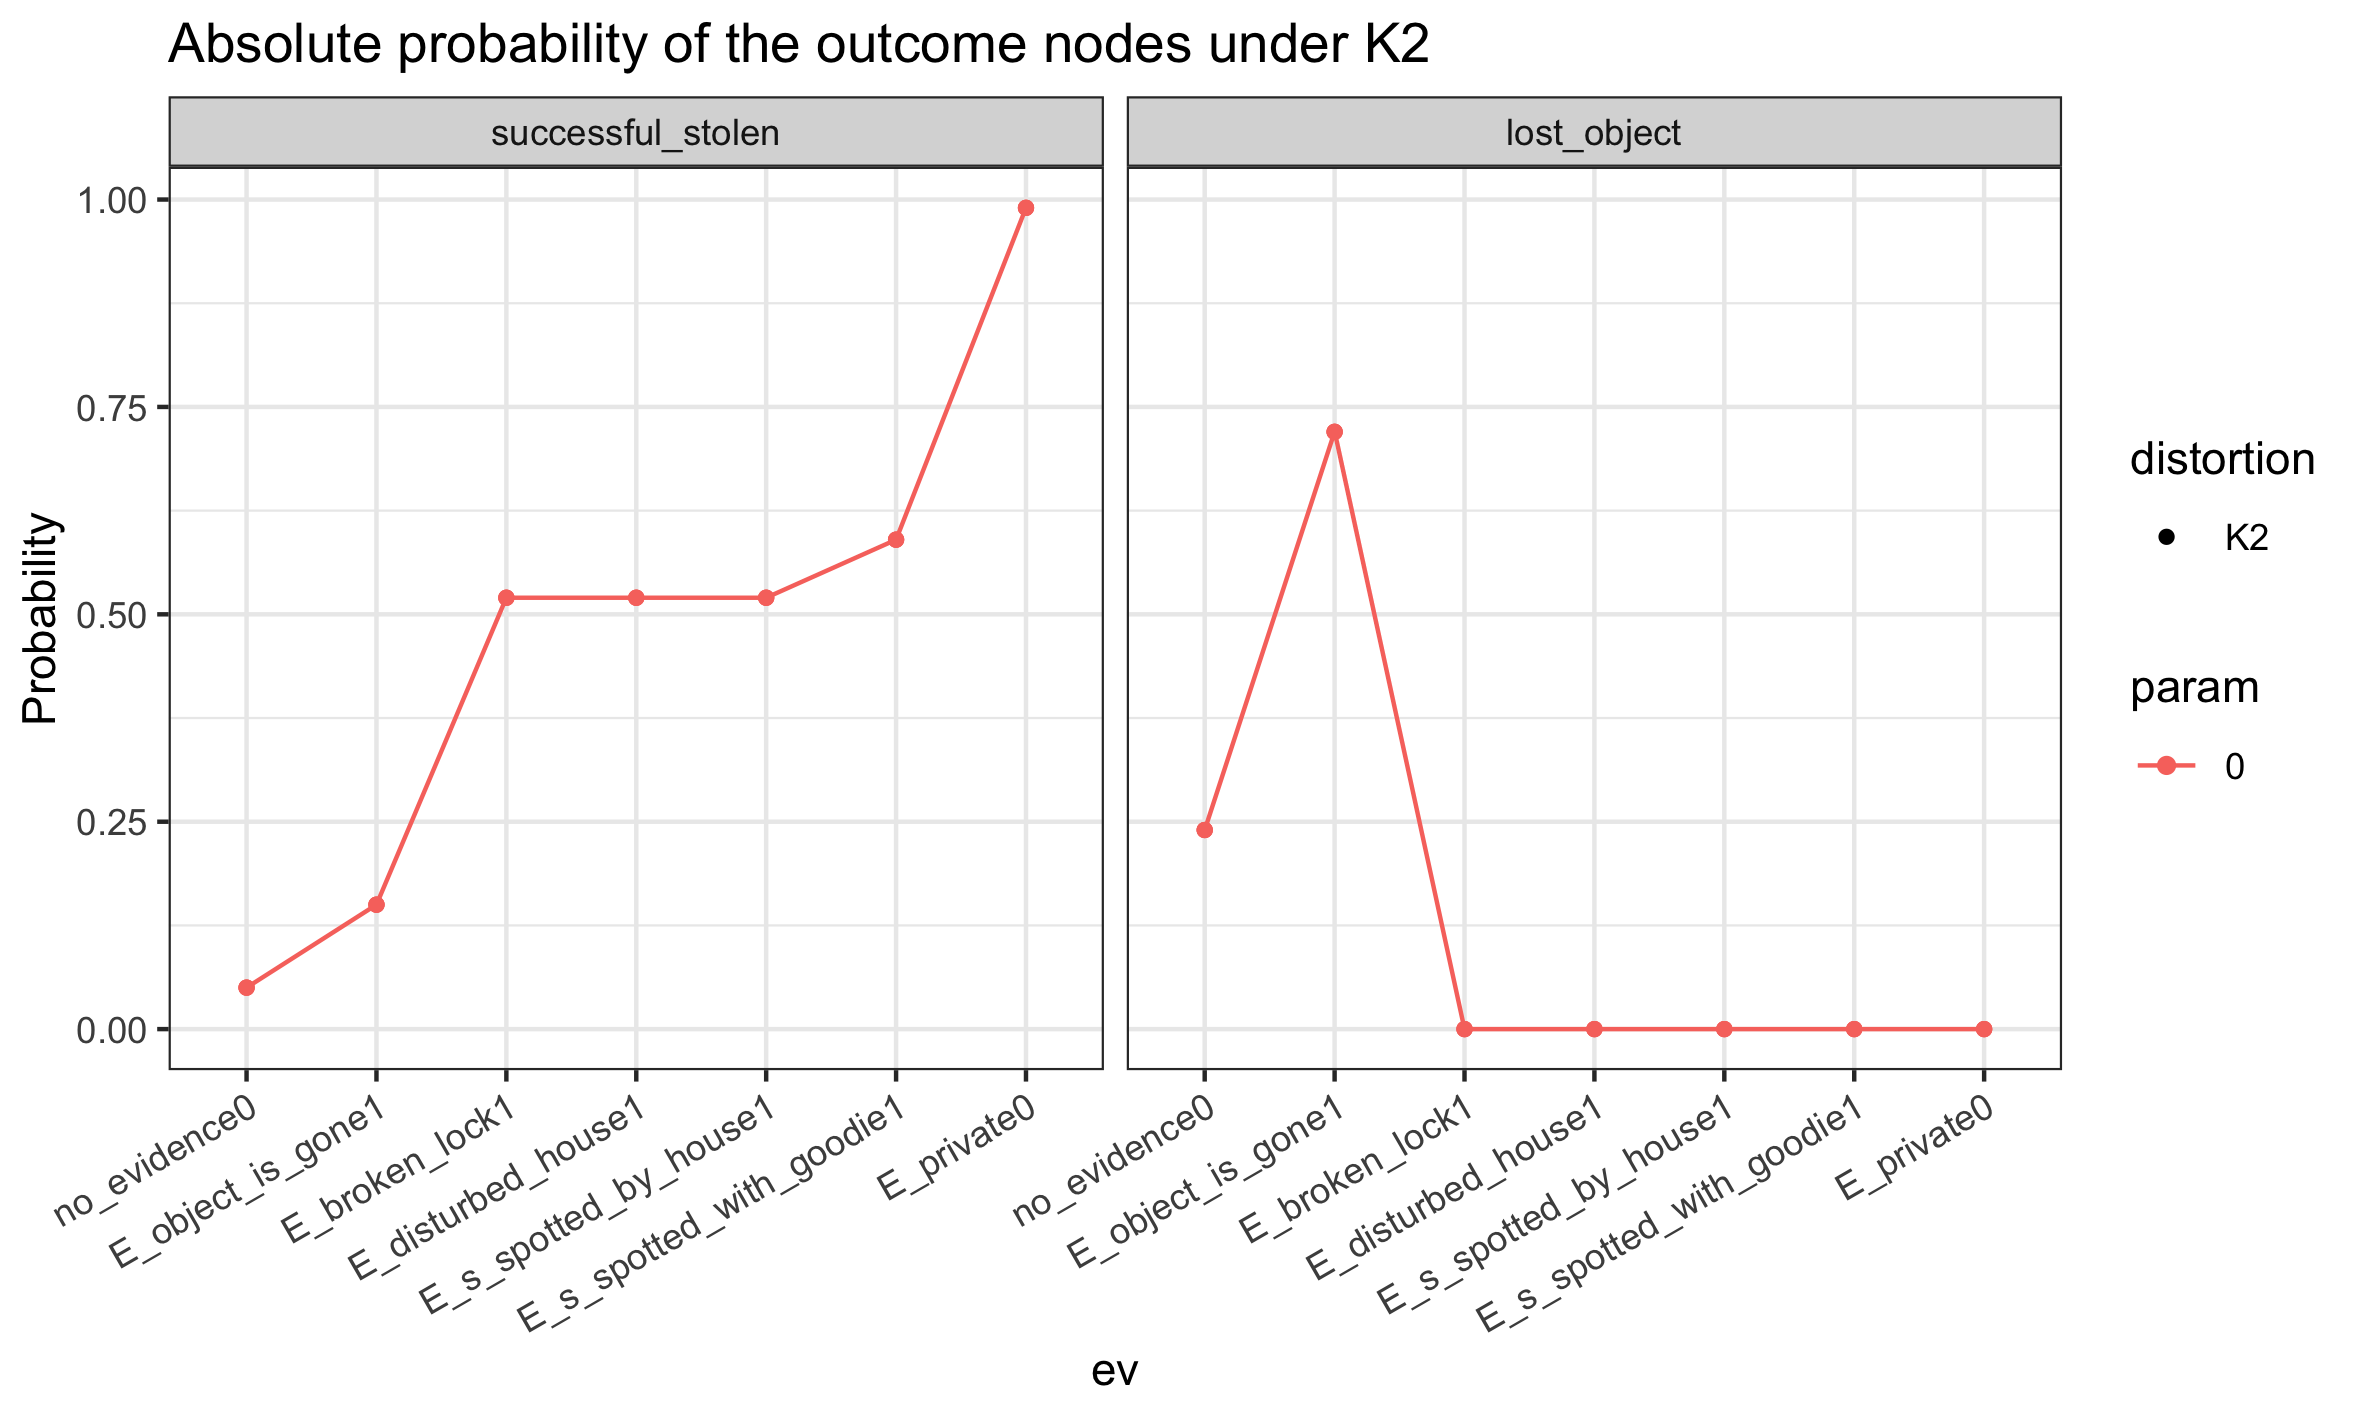
\includegraphics[width=\linewidth]{images/K2absolute.png}
\caption{default}
\label{default}
\end{center}
\end{figure}
\begin{figure}[htbp]
\centering
\begin{center}
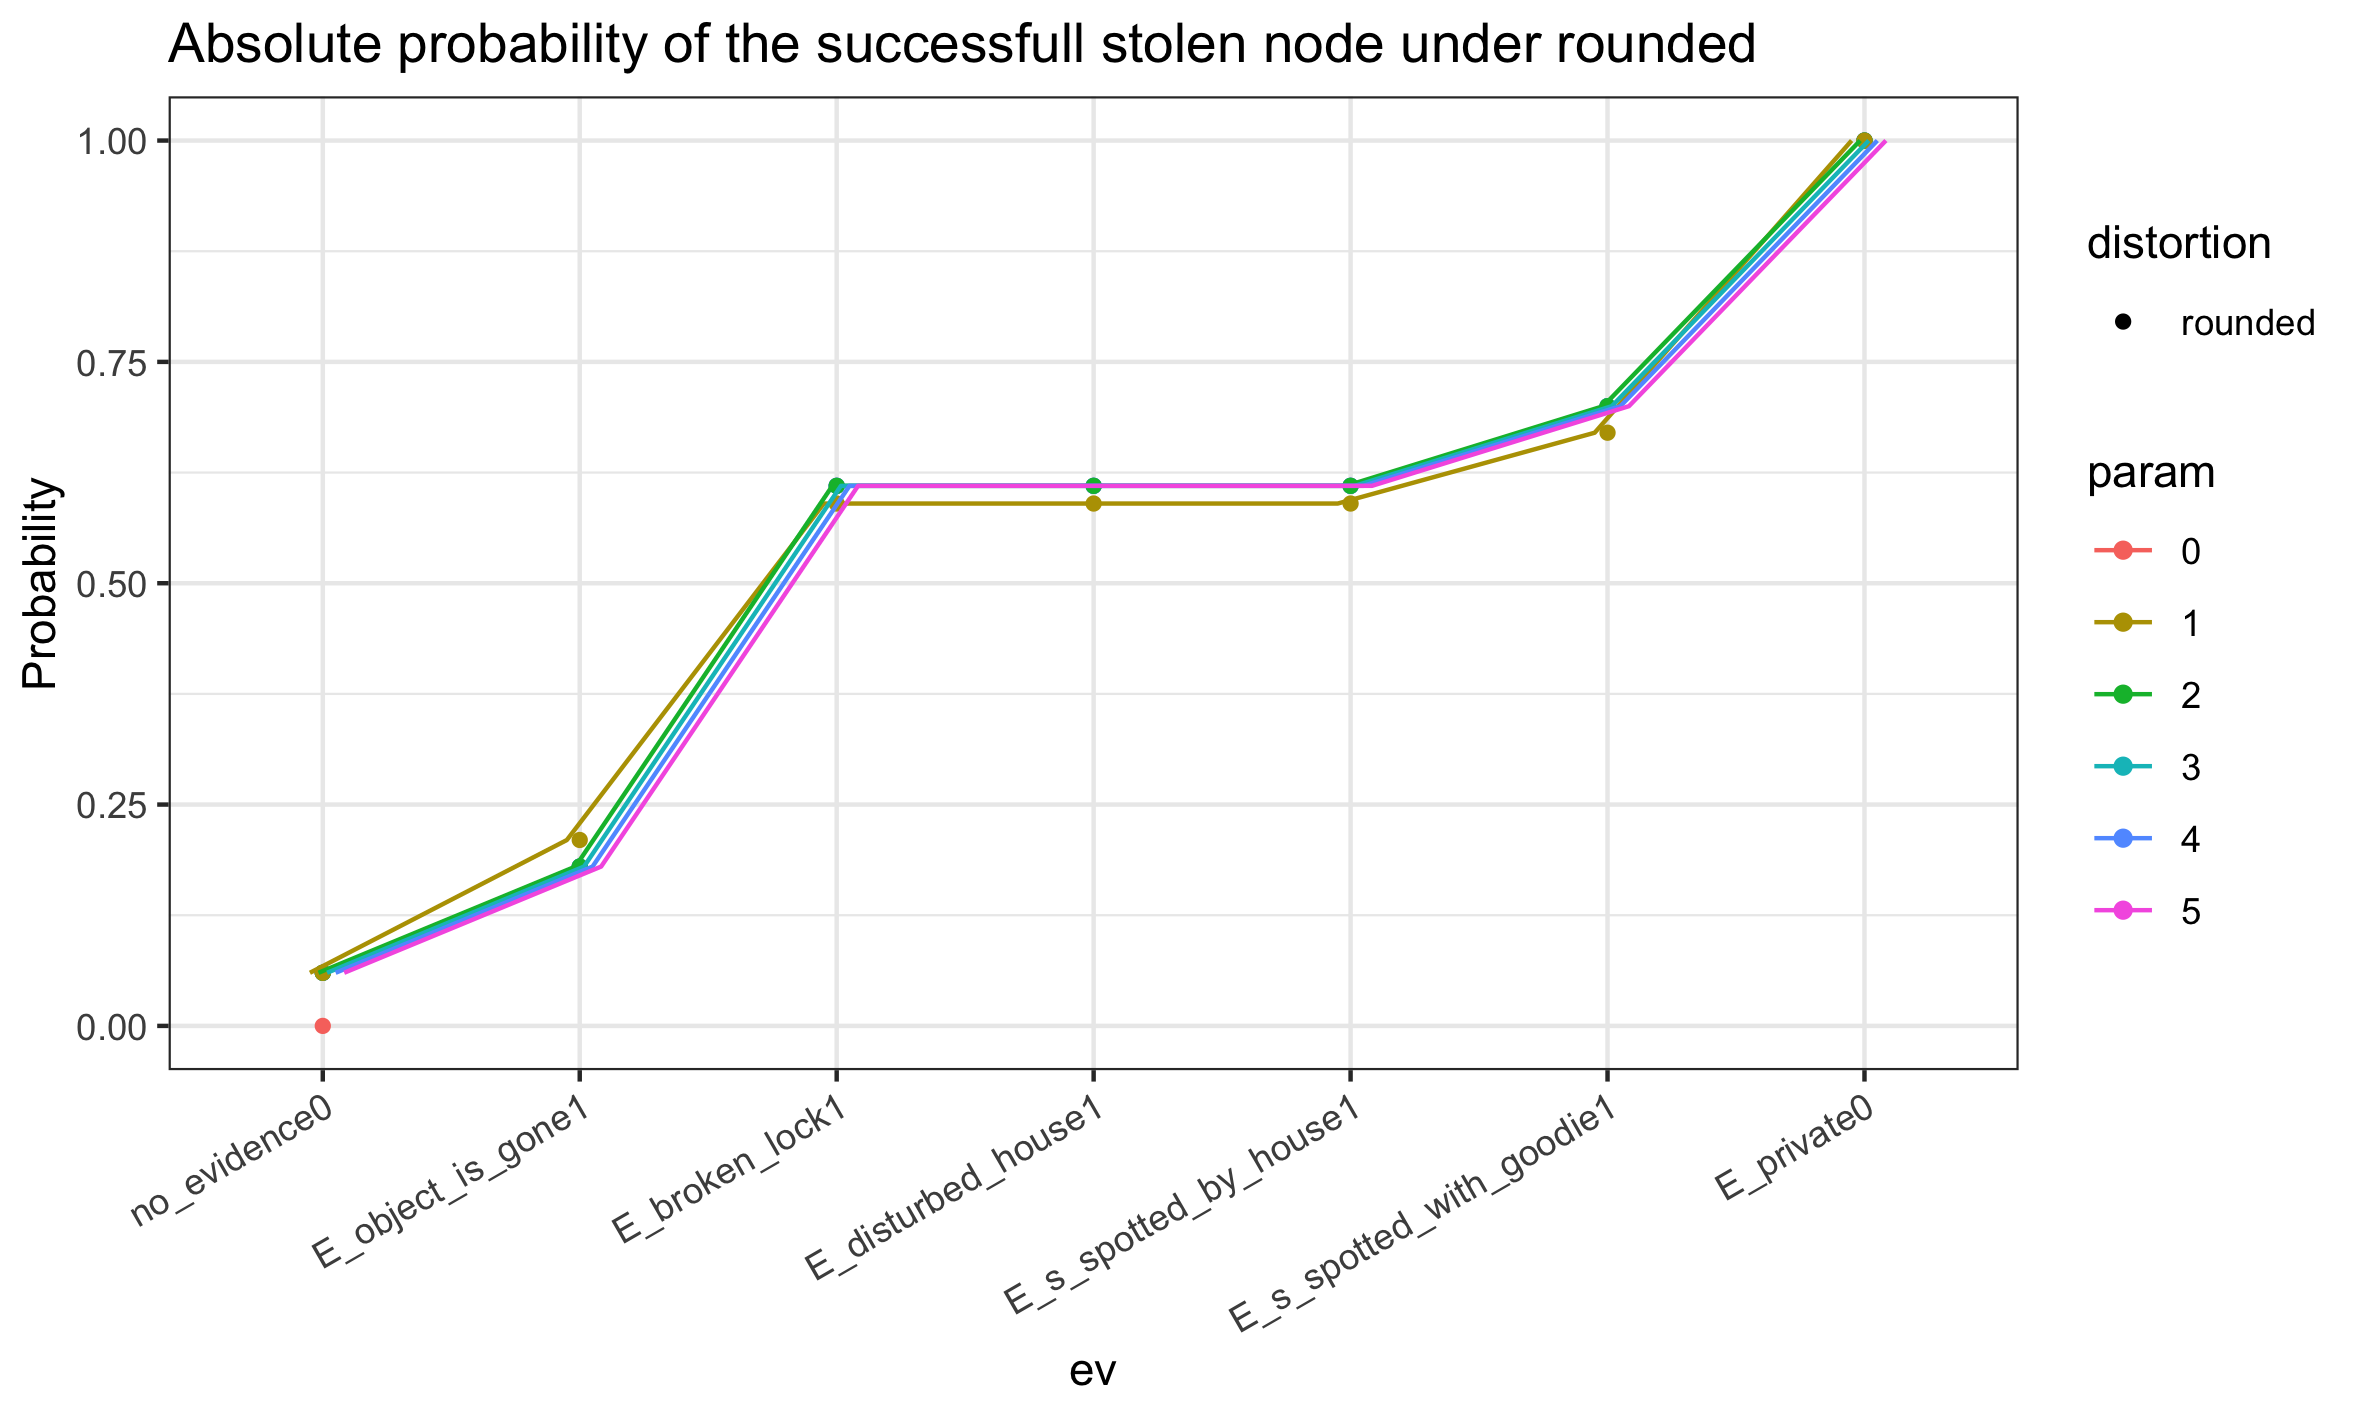
\includegraphics[width=\linewidth]{images/roundedabsolute.png}
\caption{default}
\label{default}
\end{center}
\end{figure}
\begin{figure}[htbp]
\centering
\begin{center}
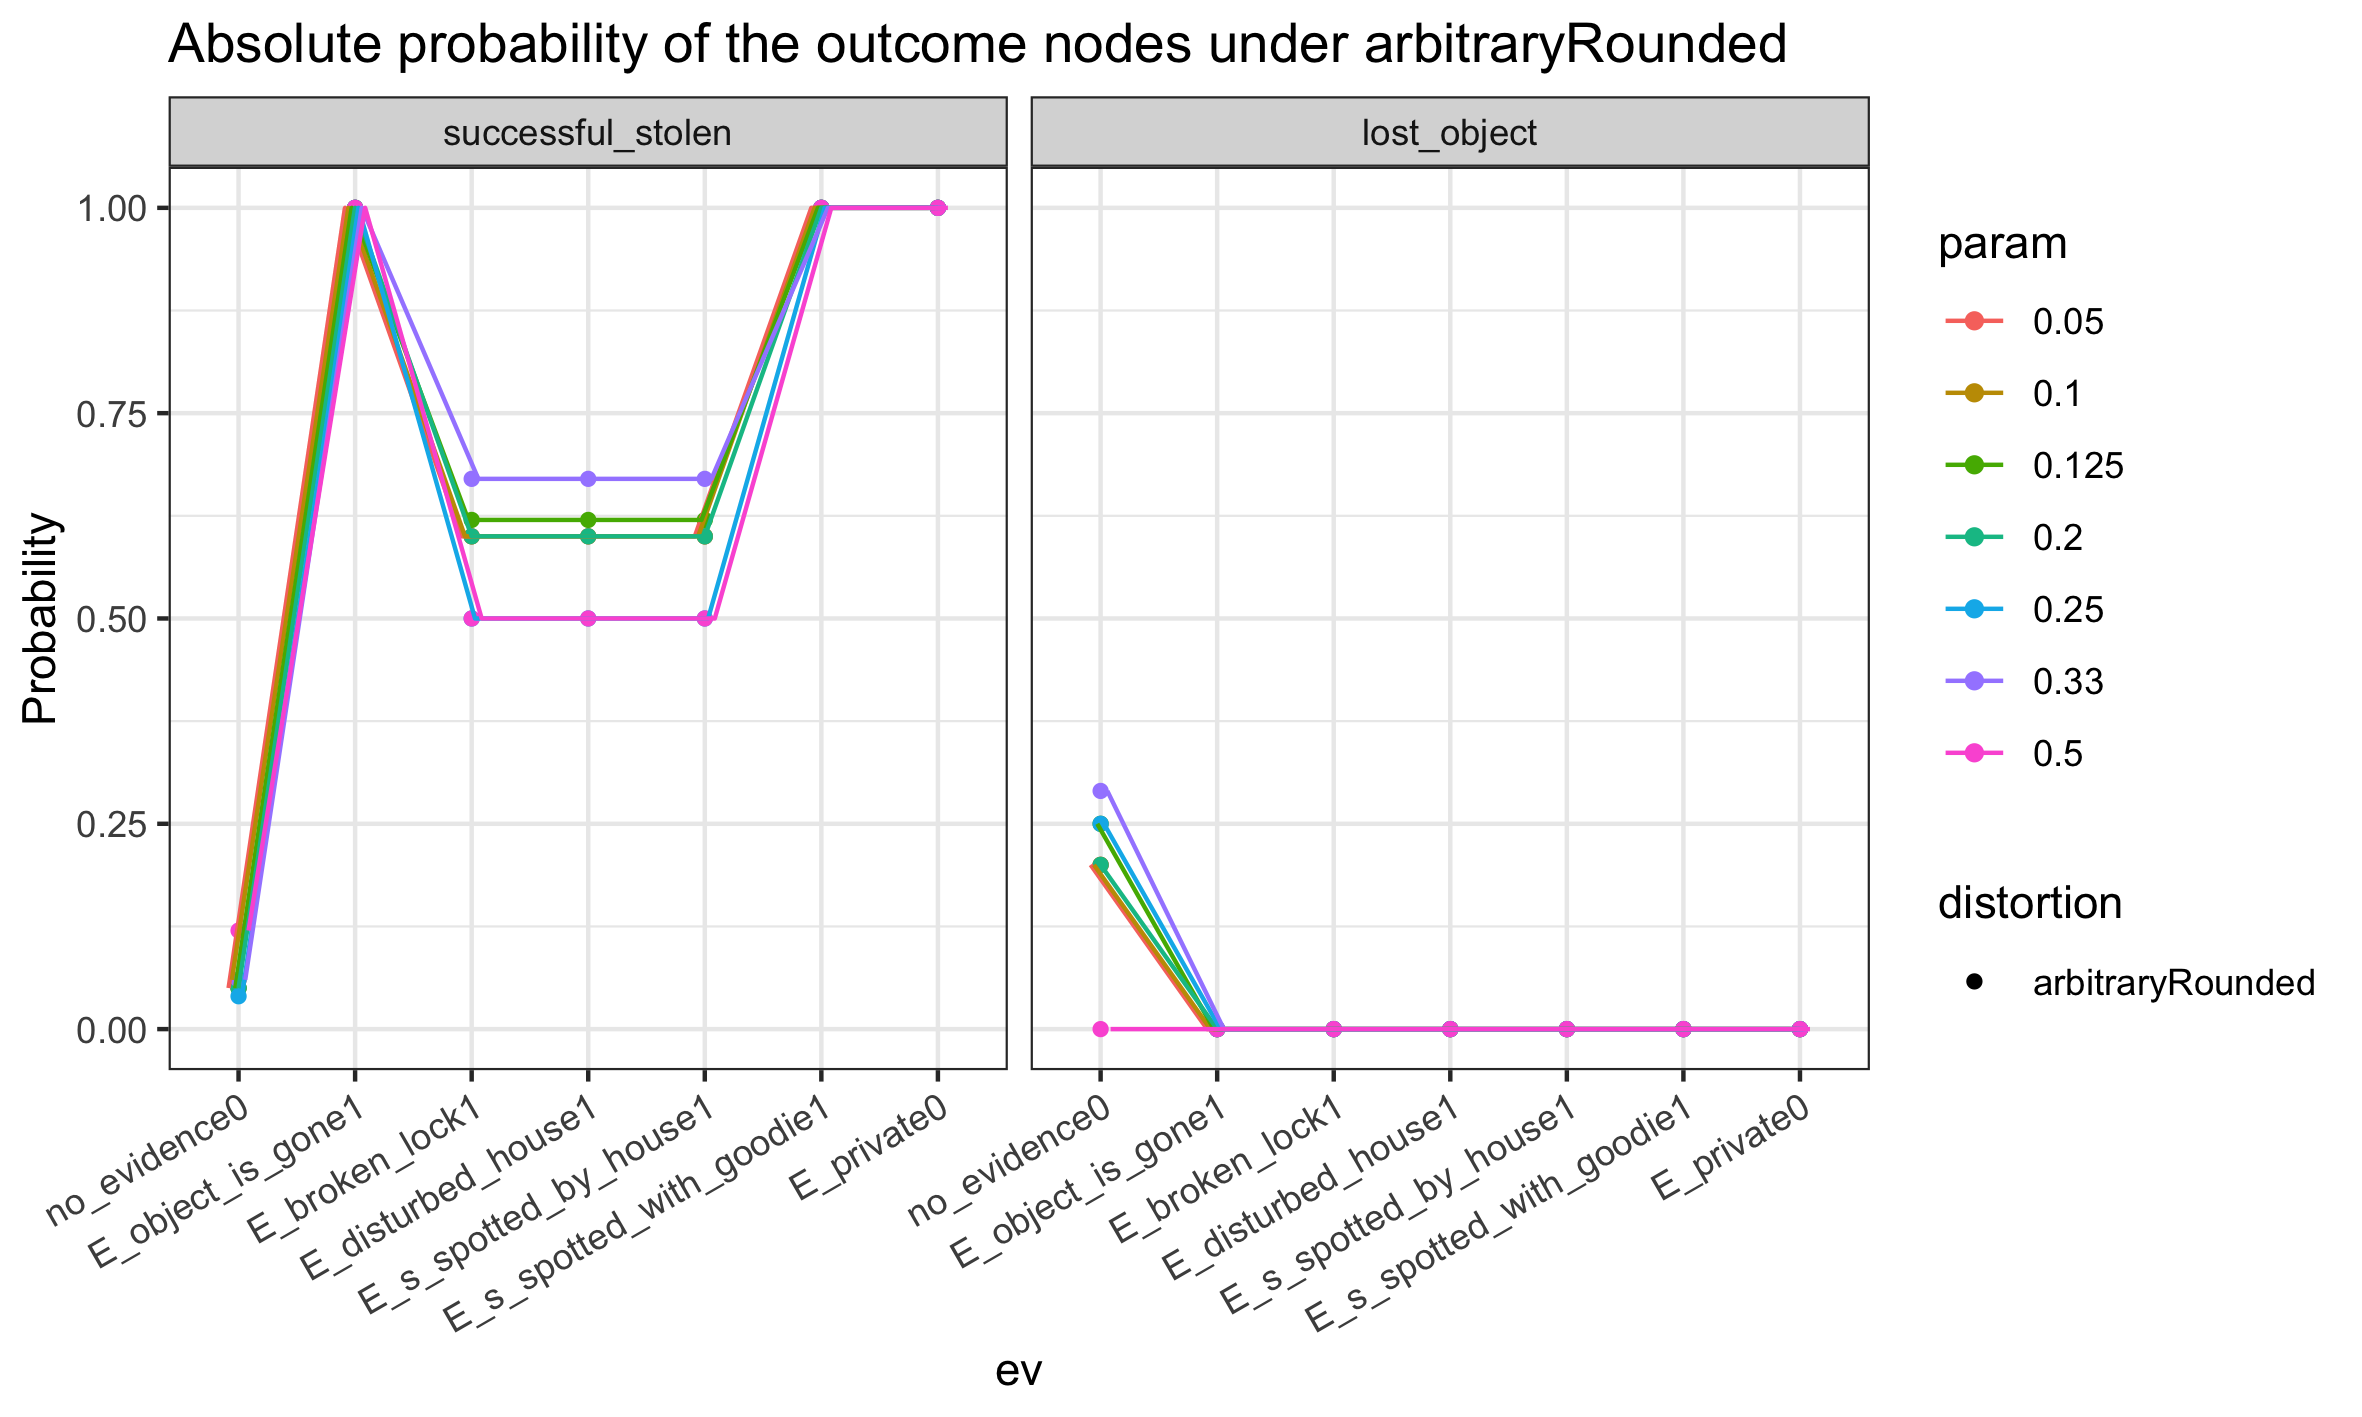
\includegraphics[width=\linewidth]{images/arbitraryRoundedabsolute.png}
\caption{default}
\label{default}
\end{center}
\end{figure}
\begin{figure}[htbp]
\centering
\begin{center}
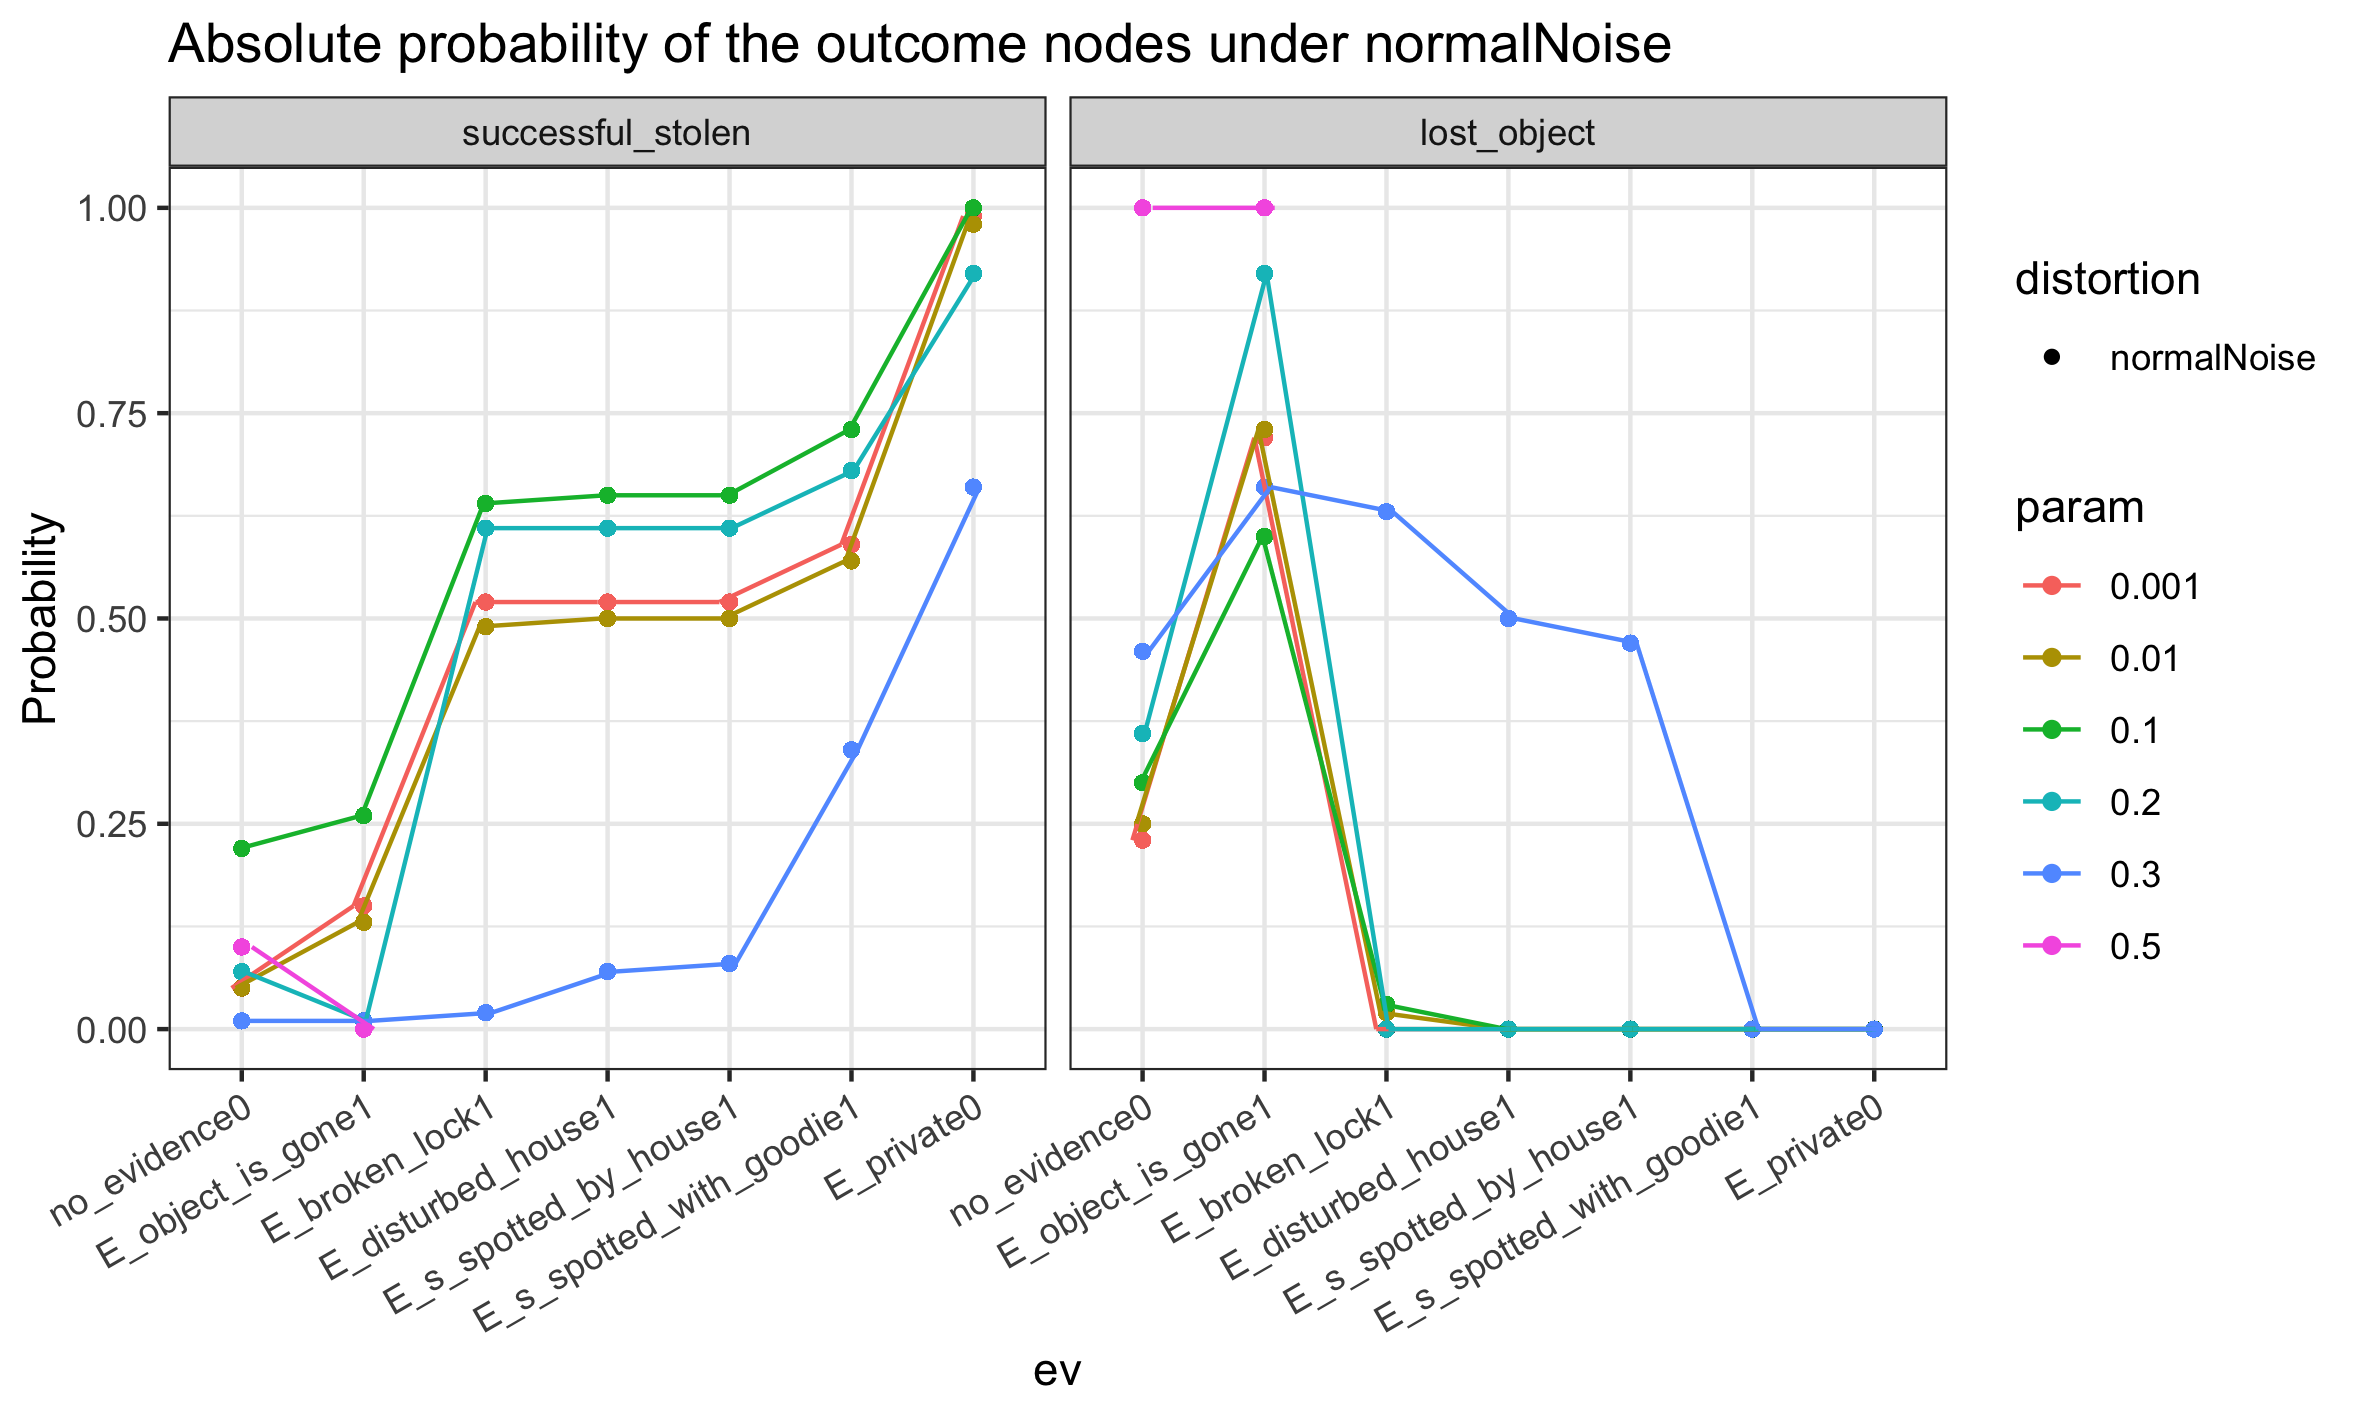
\includegraphics[width=\linewidth]{images/normalNoiseabsolute.png}
\caption{default}
\label{default}
\end{center}
\end{figure}


\begin{figure}[htbp]
\begin{center}
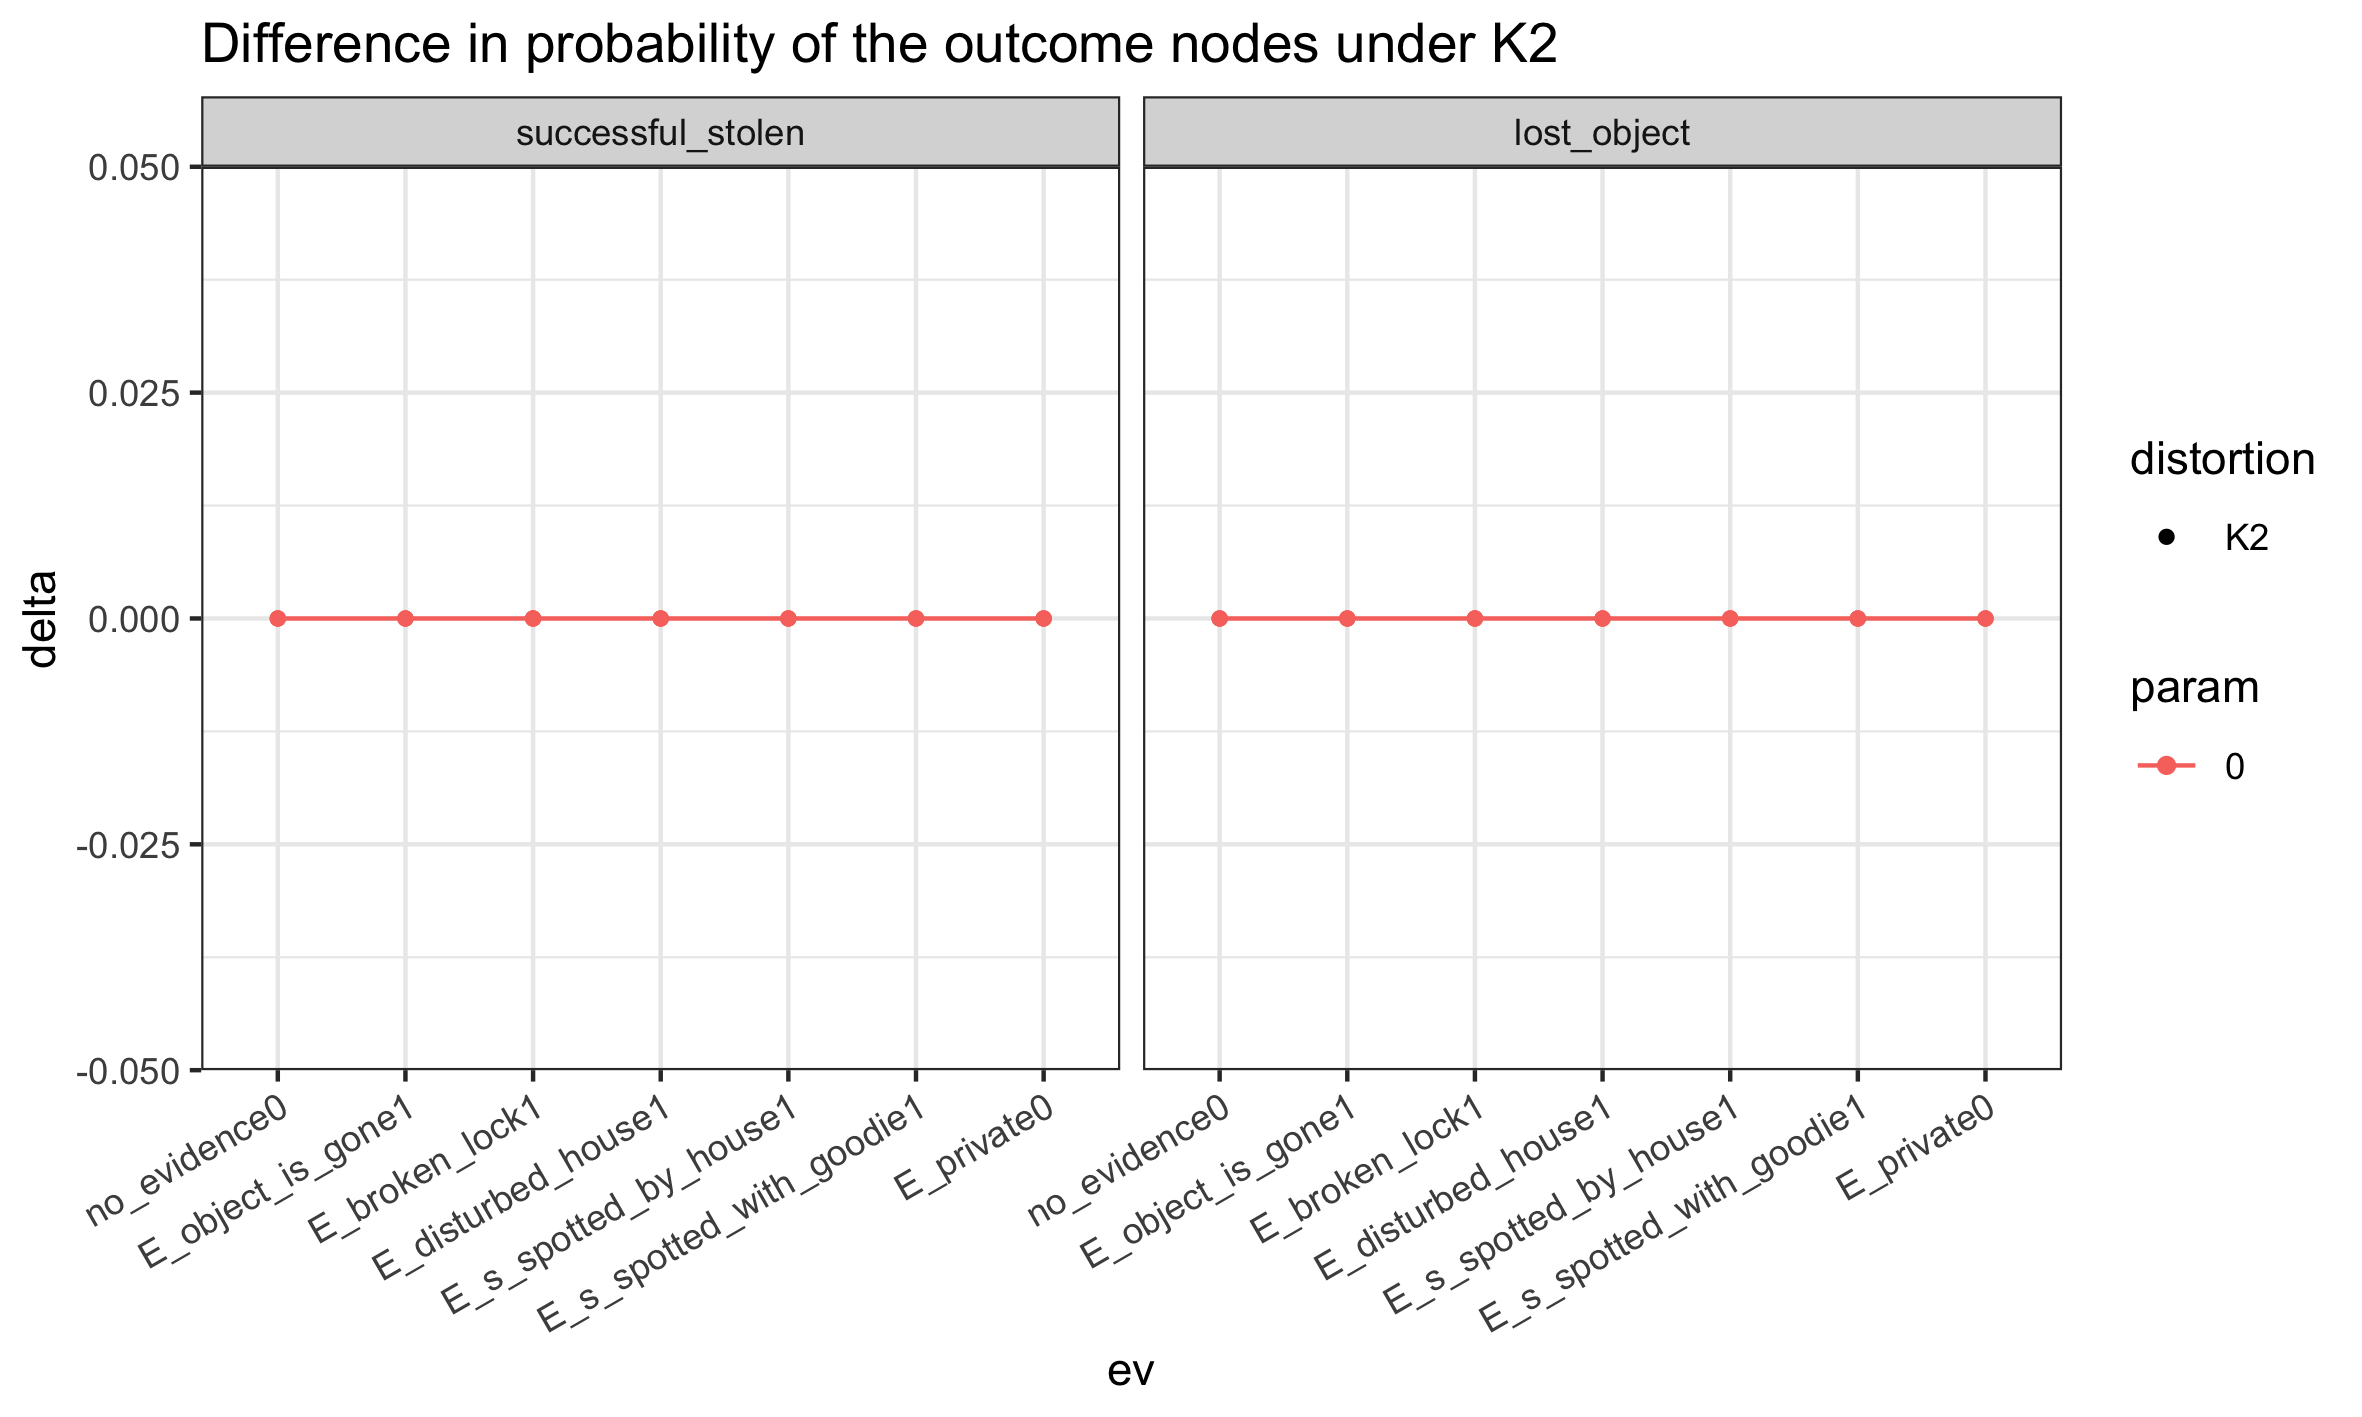
\includegraphics[width=\linewidth]{images/K2delta.png}
\caption{default}
\label{default}
\end{center}
\end{figure}

\begin{figure}[htbp]
\begin{center}
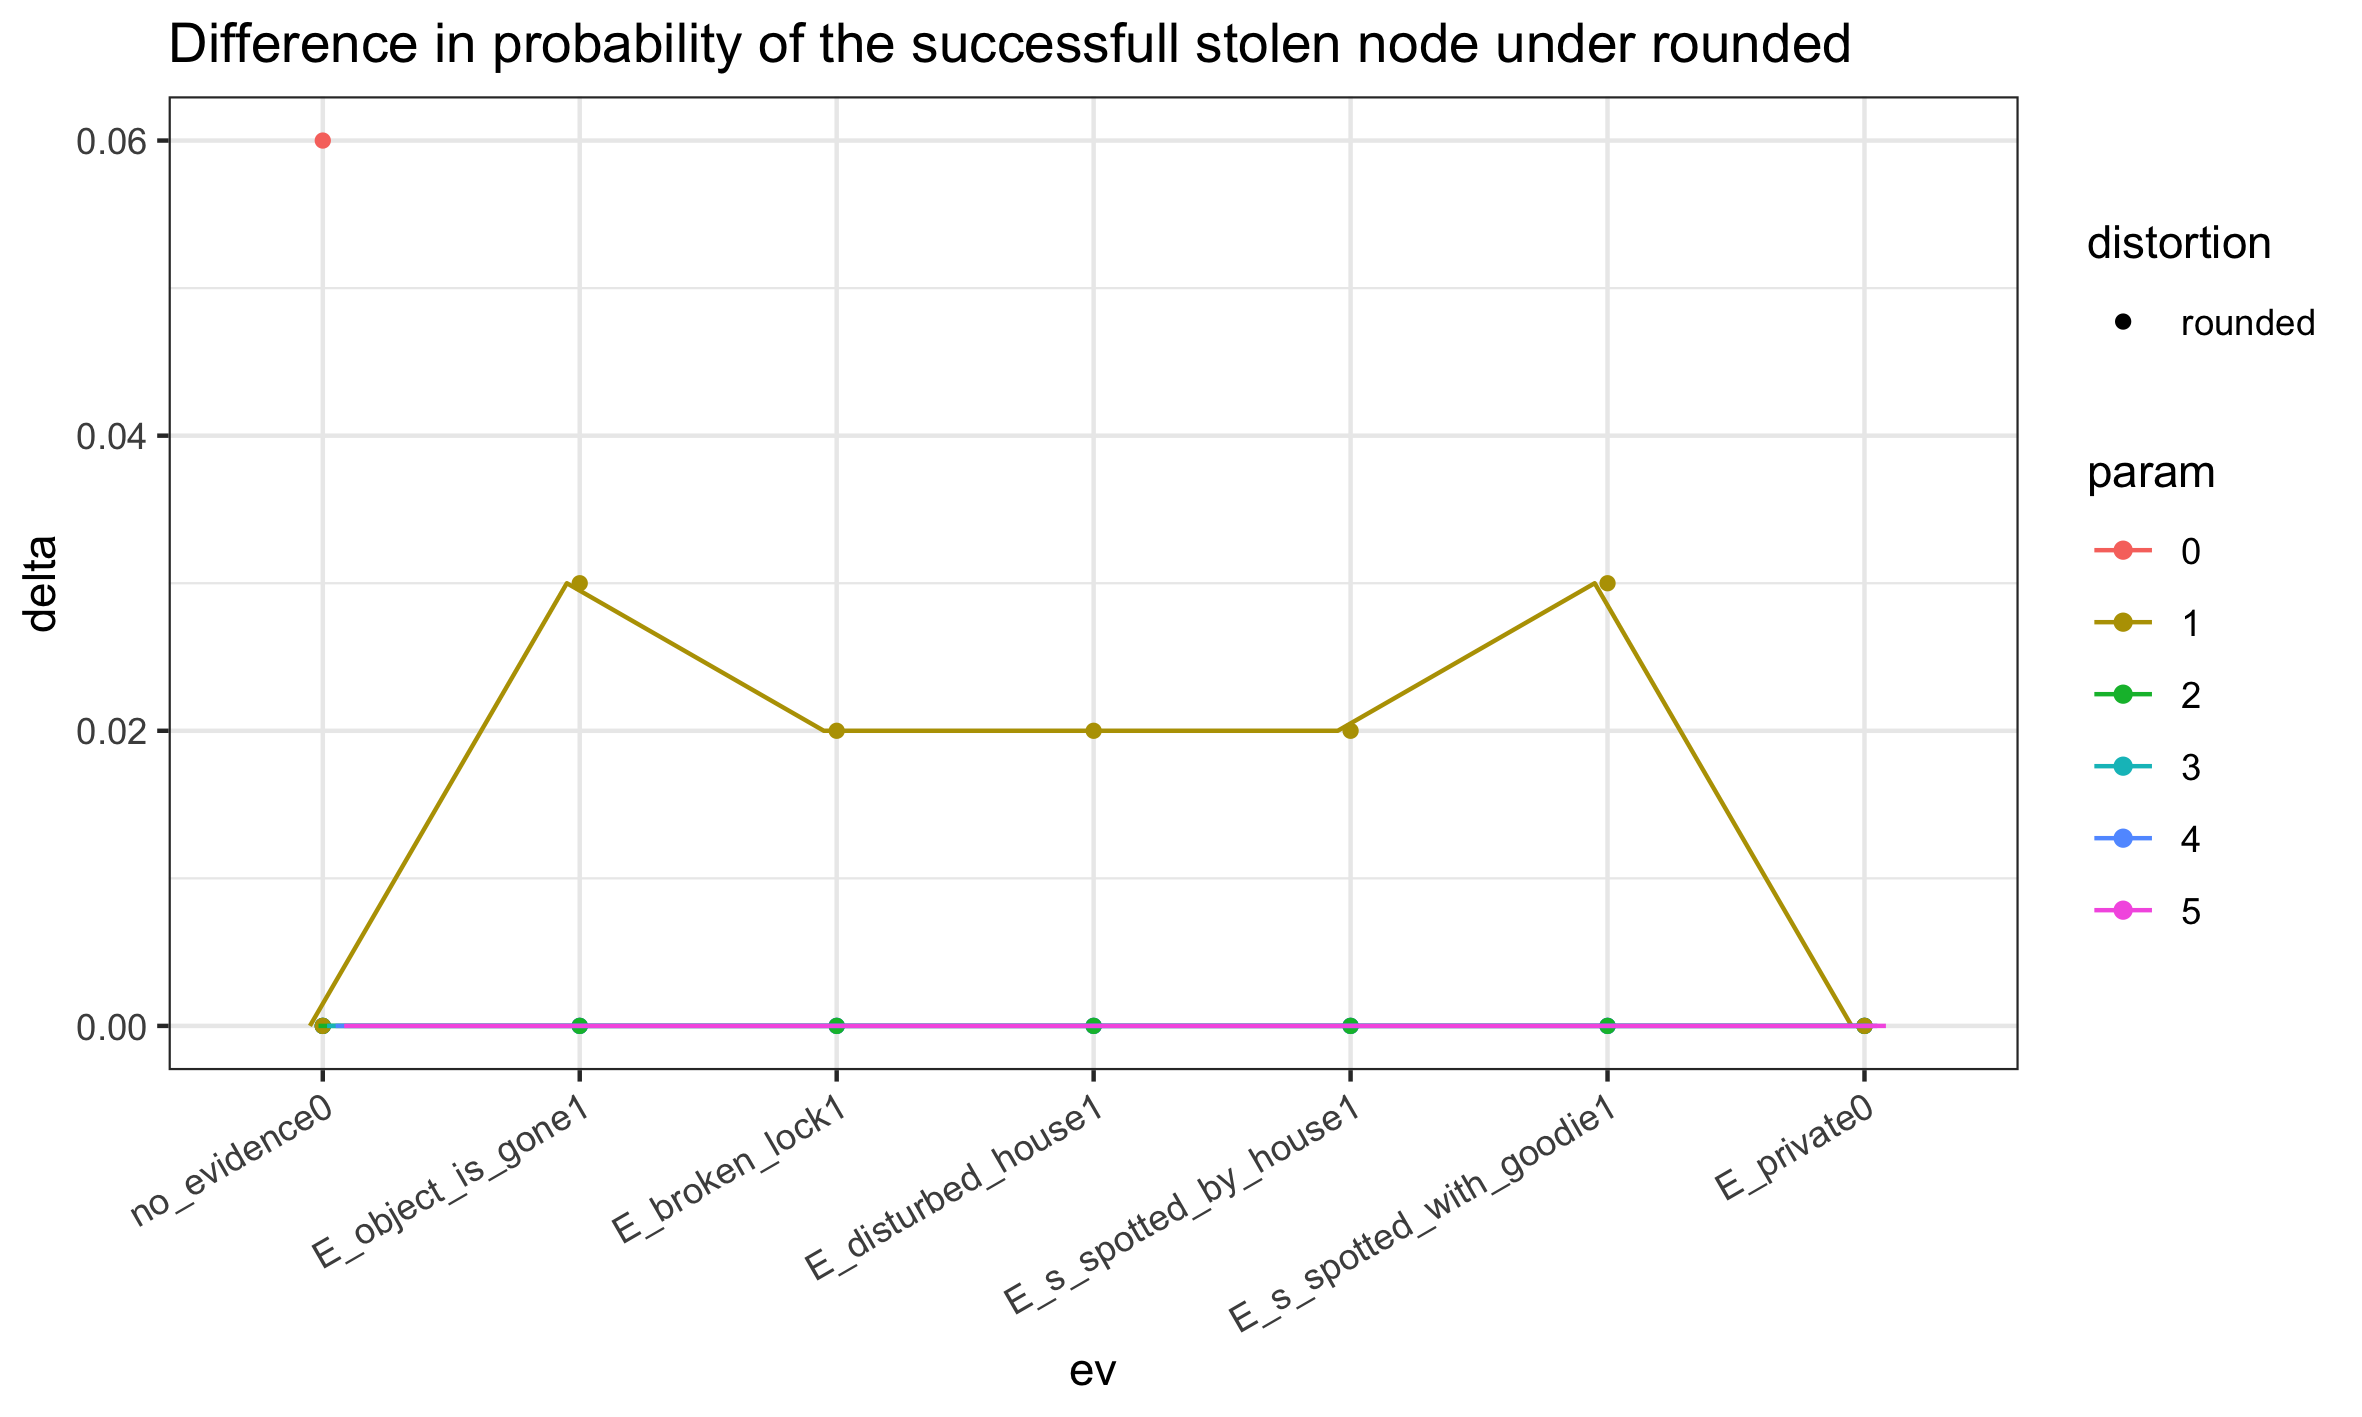
\includegraphics[width=\linewidth]{images/roundeddelta.png}
\caption{default}
\label{default}
\end{center}
\end{figure}

\begin{figure}[htbp]
\begin{center}
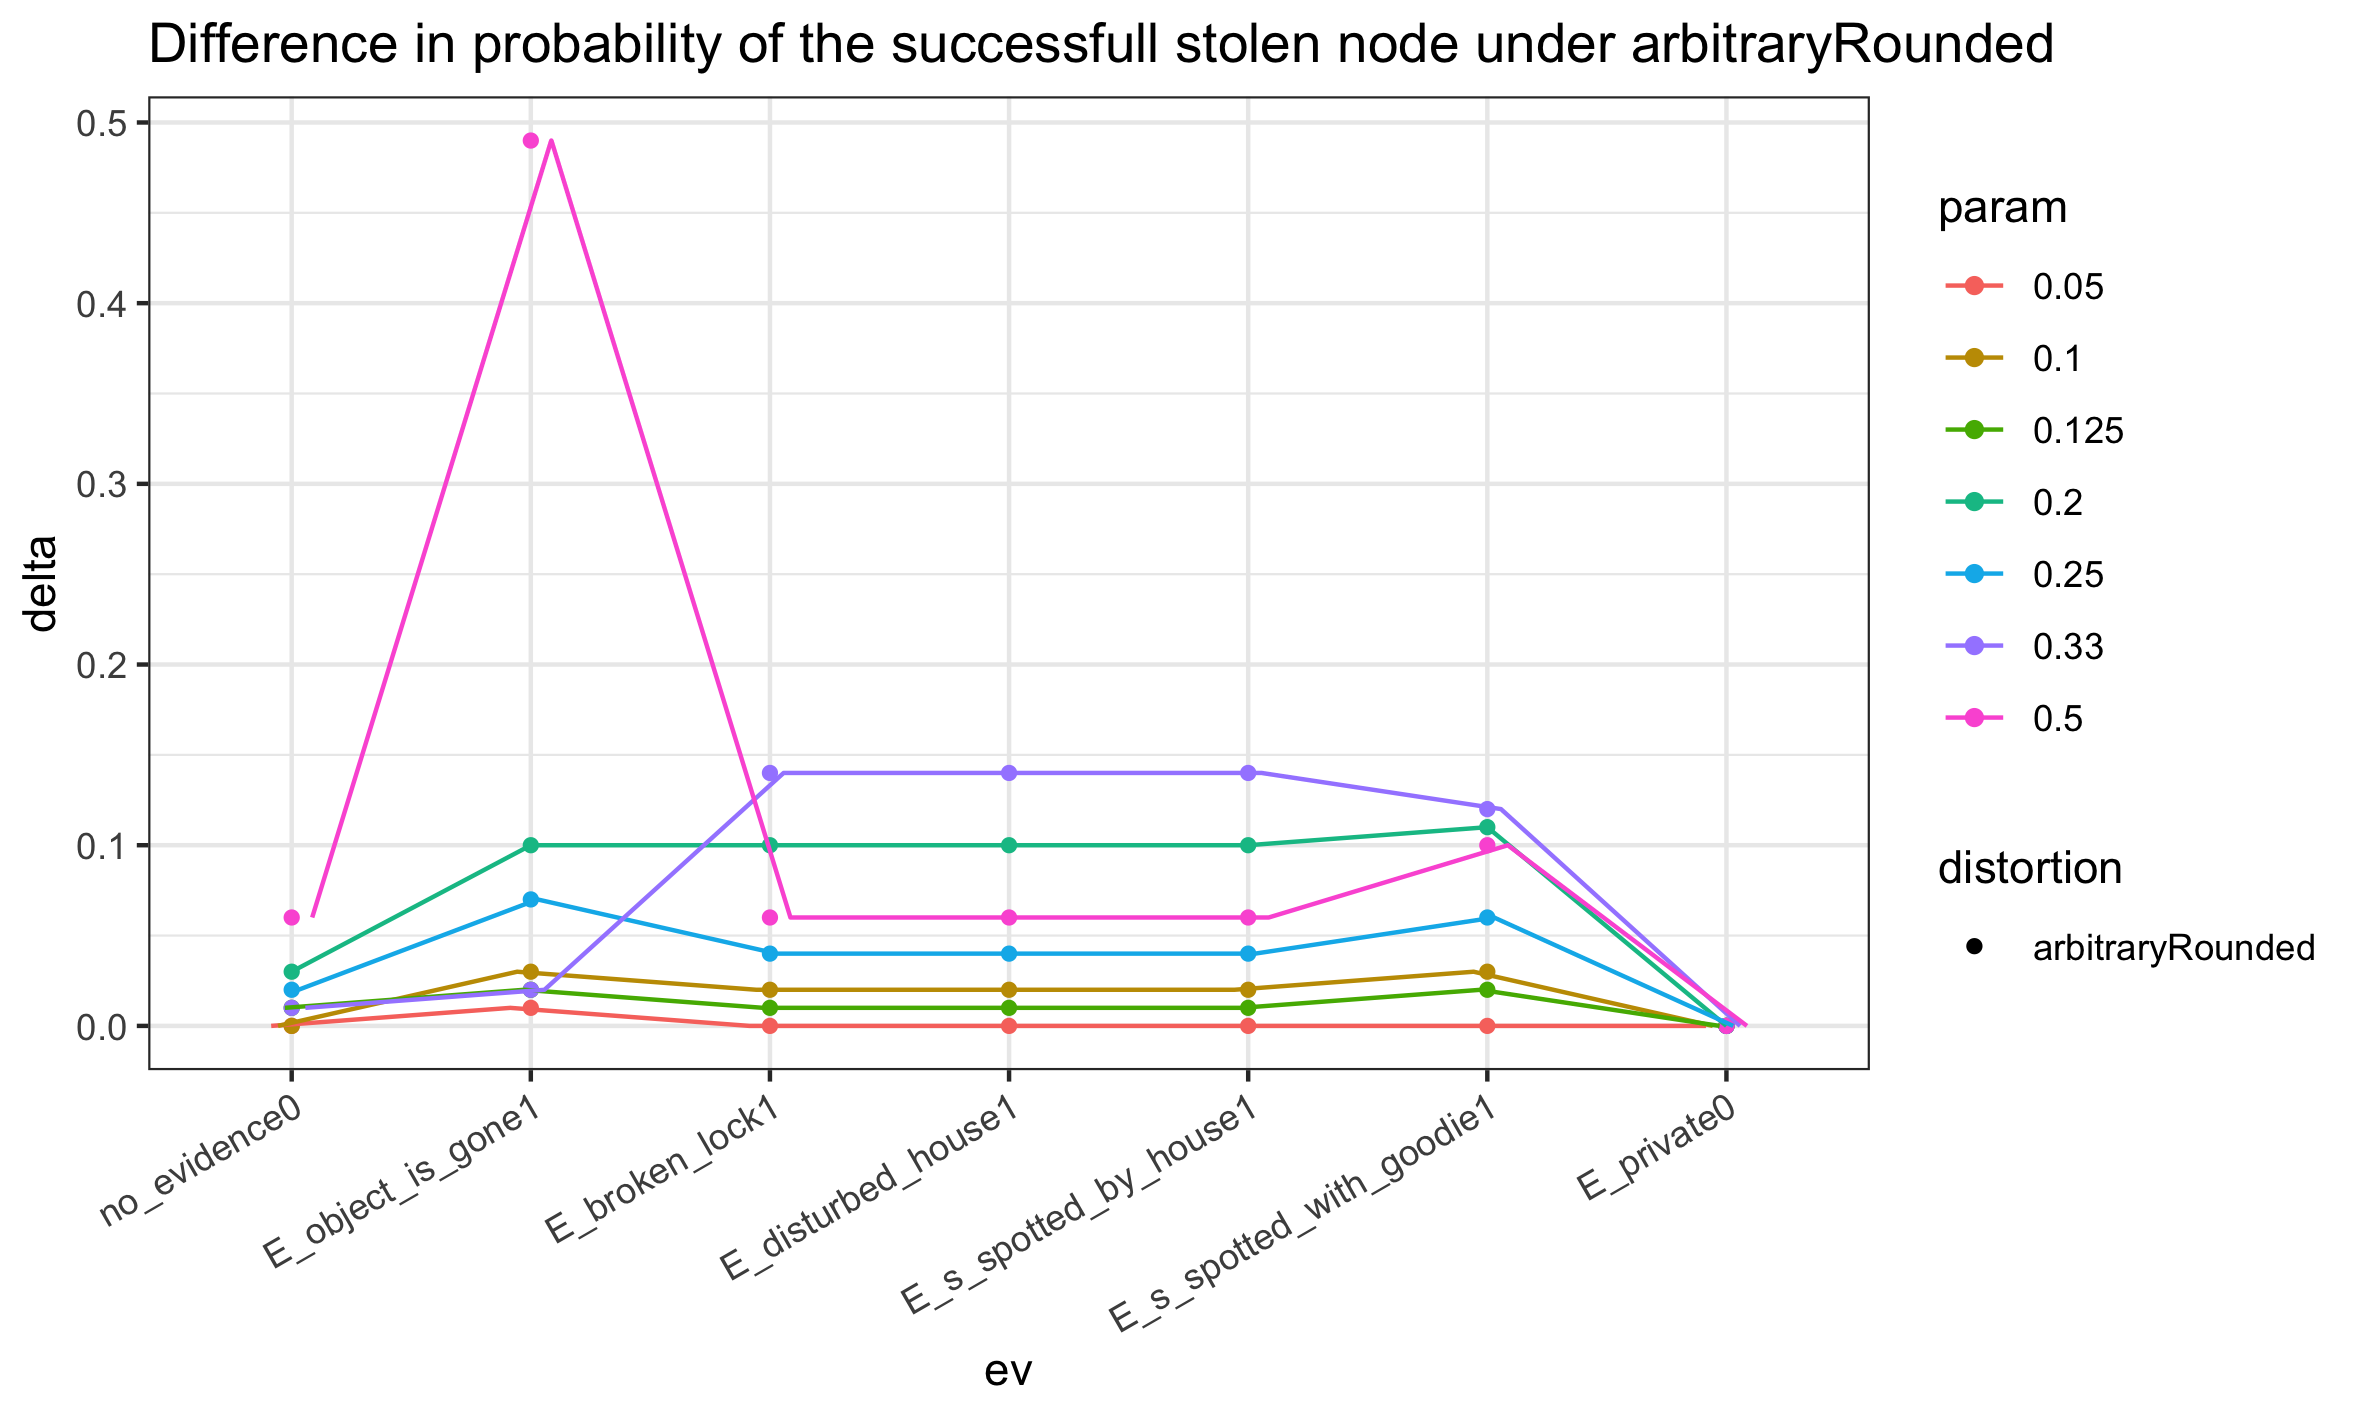
\includegraphics[width=\linewidth]{images/arbitraryRoundeddelta.png}
\caption{default}
\label{default}
\end{center}
\end{figure}

\begin{figure}[htbp]
\begin{center}
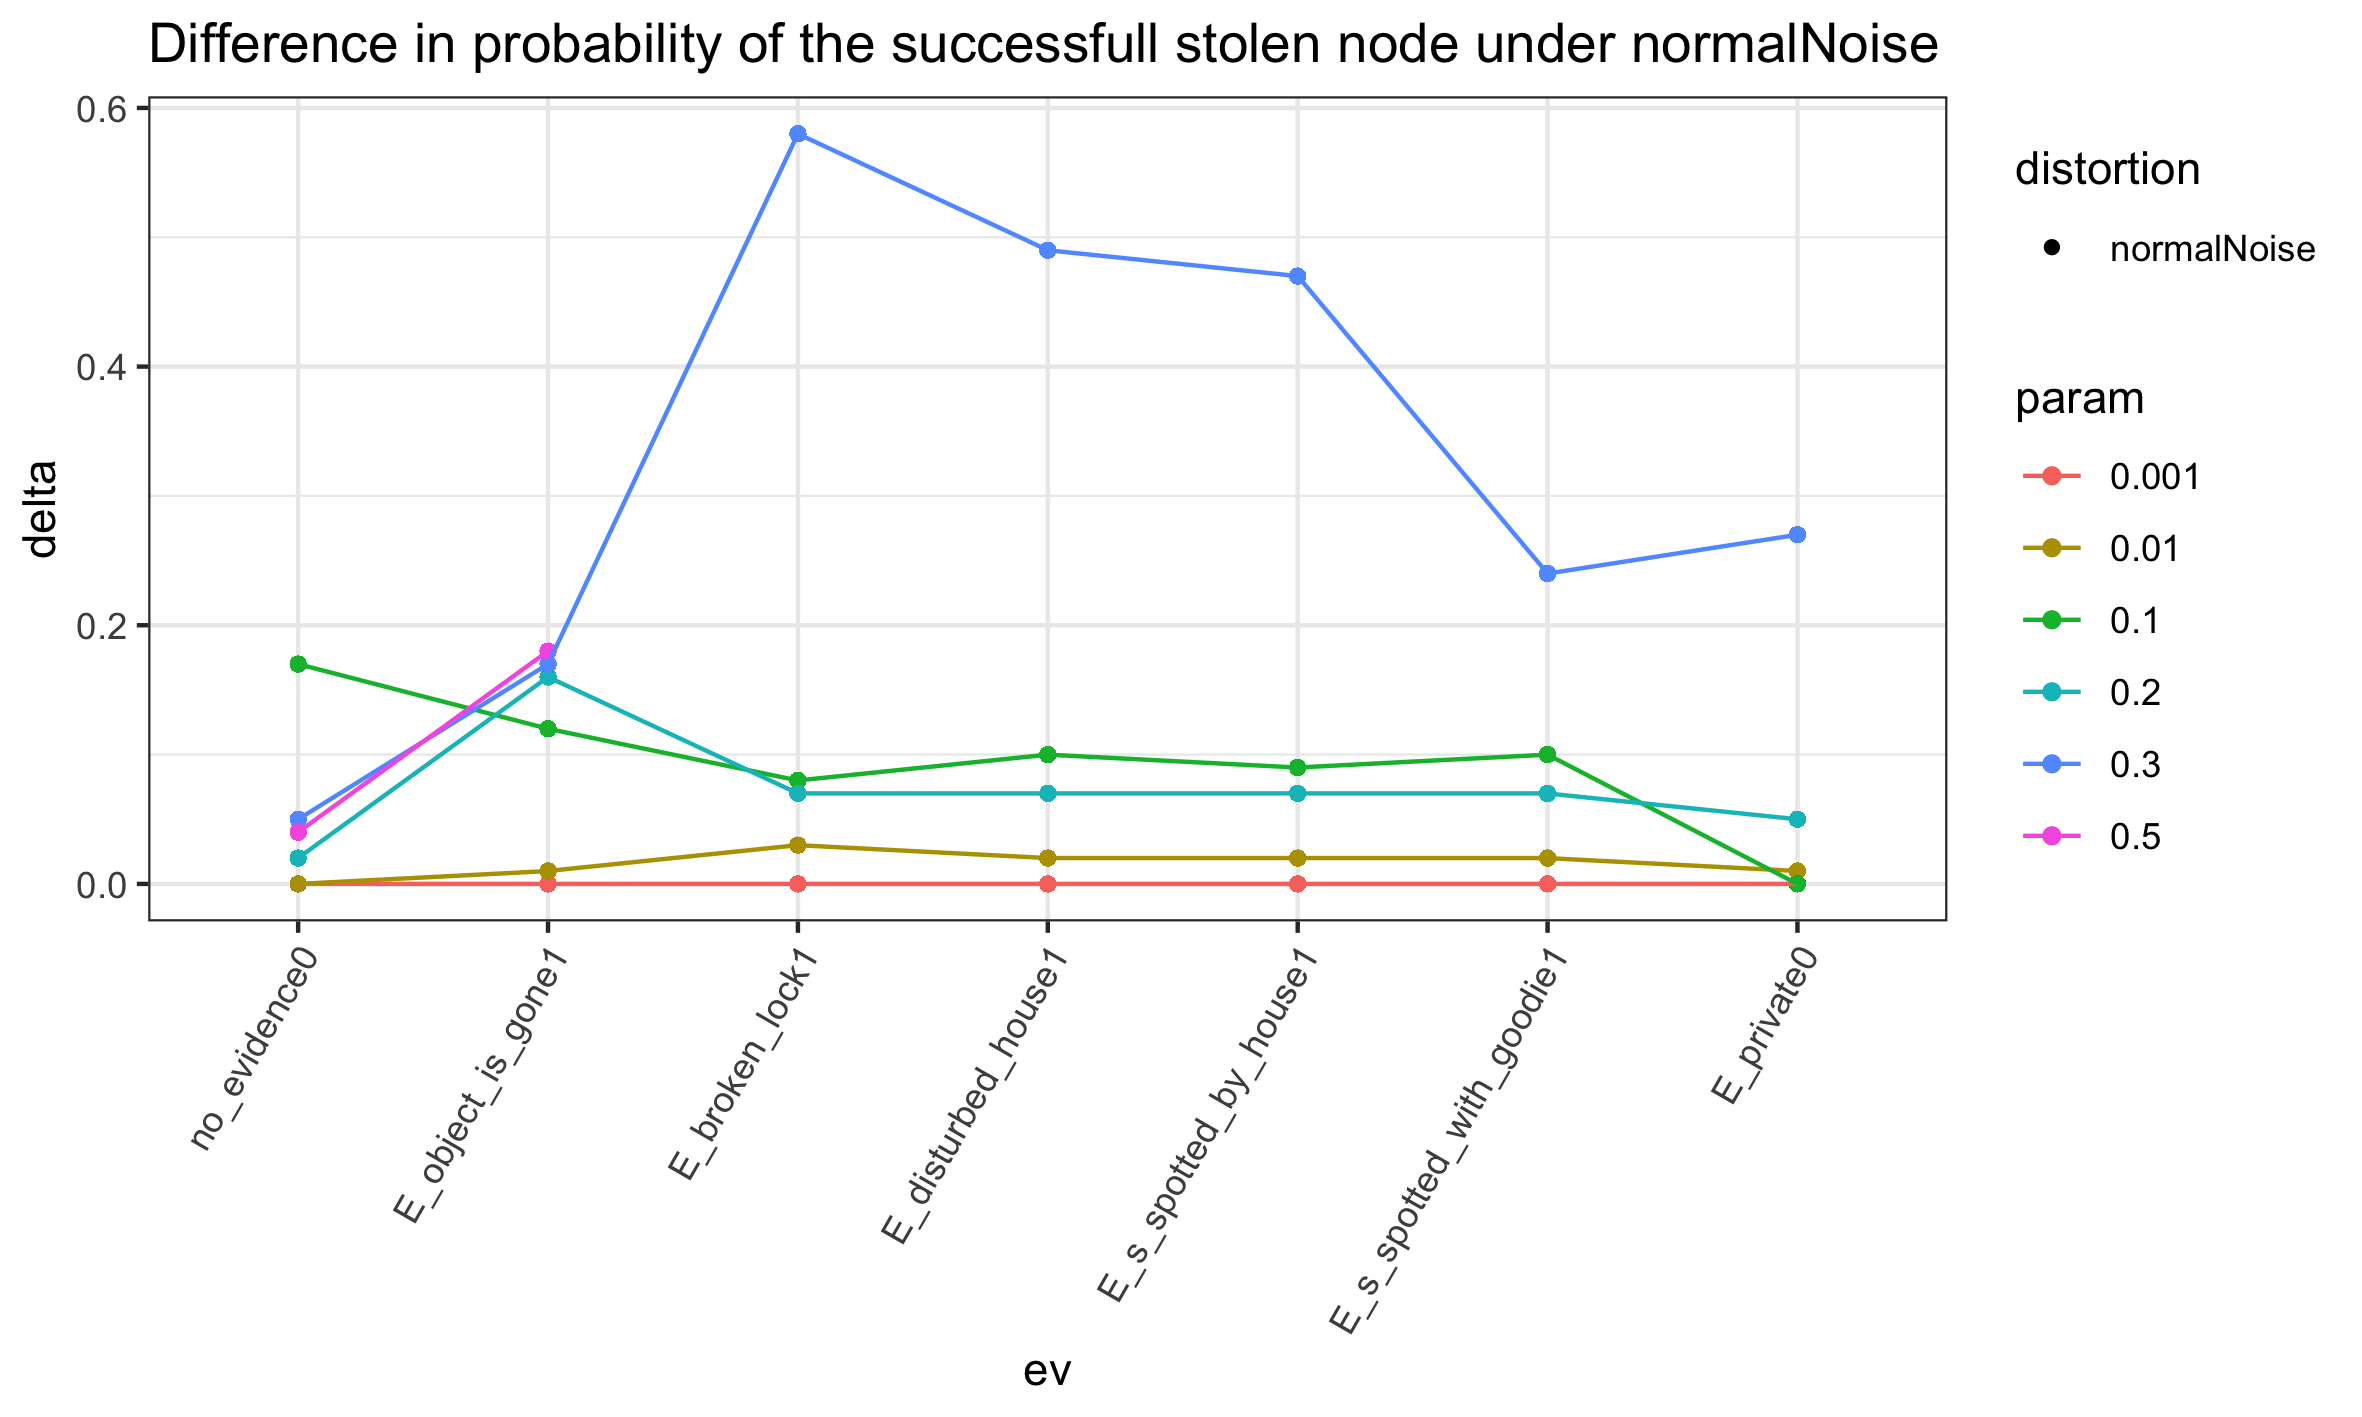
\includegraphics[width=\linewidth]{images/normalNoisedelta.png}
\caption{default}
\label{default}
\end{center}
\end{figure}


\clearpage

%\subsection{}
\section{Effect of disturbing the cpts by removing precision with rounding}
\let\oldcentering\centering
\renewcommand\centering{\tiny\oldcentering}
\begin{table}\begin{tabular}{l|cc|cc|cc|cc|cc|cc|cc}\toprule\multirow{2}{*}{Evidence} & \multicolumn{2}{c}{curtains}& \multicolumn{2}{c}{raining}& \multicolumn{2}{c}{know object}& \multicolumn{2}{c}{target object}& \multicolumn{2}{c}{motive}& \multicolumn{2}{c}{compromise house}& \multicolumn{2}{c}{flees startled}\\& {K2} & {Dev}& {K2} & {Dev}& {K2} & {Dev}& {K2} & {Dev}& {K2} & {Dev}& {K2} & {Dev}& {K2} & {Dev}\\\midrule
no evidence, 0 & H0&H0&H1&H1&H1&H1&H0&H0&H0&H0&H0&H0&H0&H0\\E object is gone, 1 & H0&H0&H1&H1&H0&H0&H0&H0&H0&H0&H0&H0&H0&H0\\E broken lock, 1 & H0&H0&H1&H1&H1&H1&H1&H1&H1&H1&H1&H1&H0&H0\\E disturbed house, 1 & H0&H0&H1&H1&H1&H1&H1&H1&H1&H1&H1&H1&H0&H0\\E s spotted by house, 1 & H0&H0&H1&H1&H1&H1&H1&H1&H1&H1&H1&H1&H0&H0\\E s spotted with goodie, 1 & H0&H0&H1&H1&H1&H1&H1&H1&H1&H1&H1&H1&H0&H0\\E private, 0 & H0&H0&H1&H1&H1&H1&H1&H1&H1&H1&H1&H1&H0&H0\\\bottomrule\end{tabular}\caption{Effect of disturbance of [5, 'decimal places'] on weak view of outcomes.}\end{table}
\begin{table}\begin{tabular}{l|cc|cc|cc|cc|cc|cc|cc}\toprule\multirow{2}{*}{Evidence} & \multicolumn{2}{c}{curtains}& \multicolumn{2}{c}{raining}& \multicolumn{2}{c}{know object}& \multicolumn{2}{c}{target object}& \multicolumn{2}{c}{motive}& \multicolumn{2}{c}{compromise house}& \multicolumn{2}{c}{flees startled}\\& {K2} & {Dev}& {K2} & {Dev}& {K2} & {Dev}& {K2} & {Dev}& {K2} & {Dev}& {K2} & {Dev}& {K2} & {Dev}\\\midrule
no evidence, 0 & H0&H0&H1&H1&H1&H1&H0&H0&H0&H0&H0&H0&H0&H0\\E object is gone, 1 & H0&H0&H1&H1&H0&H0&H0&H0&H0&H0&H0&H0&H0&H0\\E broken lock, 1 & H0&H0&H1&H1&H1&H1&H1&H1&H1&H1&H1&H1&H0&H0\\E disturbed house, 1 & H0&H0&H1&H1&H1&H1&H1&H1&H1&H1&H1&H1&H0&H0\\E s spotted by house, 1 & H0&H0&H1&H1&H1&H1&H1&H1&H1&H1&H1&H1&H0&H0\\E s spotted with goodie, 1 & H0&H0&H1&H1&H1&H1&H1&H1&H1&H1&H1&H1&H0&H0\\E private, 0 & H0&H0&H1&H1&H1&H1&H1&H1&H1&H1&H1&H1&H0&H0\\\bottomrule\end{tabular}\caption{Effect of disturbance of [5, 'decimal places'] on weak view of outcomes.}\end{table}
\begin{table}\begin{tabular}{l|cc|cc|cc|cc|cc|cc|cc}\toprule\multirow{2}{*}{Evidence} & \multicolumn{2}{c}{curtains}& \multicolumn{2}{c}{raining}& \multicolumn{2}{c}{know object}& \multicolumn{2}{c}{target object}& \multicolumn{2}{c}{motive}& \multicolumn{2}{c}{compromise house}& \multicolumn{2}{c}{flees startled}\\& {K2} & {Dev}& {K2} & {Dev}& {K2} & {Dev}& {K2} & {Dev}& {K2} & {Dev}& {K2} & {Dev}& {K2} & {Dev}\\\midrule
no evidence, 0 & 0.17&0.17&0.5&0.5&0.65&0.65&0.32&0.32&0.32&0.32&0.1&0.1&0.16&0.16\\E object is gone, 1 & 0.12&0.12&0.5&0.5&0.31&0.31&0.31&0.31&0.31&0.31&0.31&0.31&0.13&0.13\\E broken lock, 1 & 0.0&0.0&0.5&0.5&1.0&1.0&1.0&1.0&1.0&1.0&1.0&1.0&0.4&0.4\\E disturbed house, 1 & 0.0&0.0&0.5&0.5&1.0&1.0&1.0&1.0&1.0&1.0&1.0&1.0&0.4&0.4\\E s spotted by house, 1 & 0.0&0.0&0.5&0.5&1.0&1.0&1.0&1.0&1.0&1.0&1.0&1.0&0.4&0.4\\E s spotted with goodie, 1 & 0.0&0.0&0.5&0.5&1.0&1.0&1.0&1.0&1.0&1.0&1.0&1.0&0.32&0.32\\E private, 0 & 0.0&0.0&0.5&0.5&1.0&1.0&1.0&1.0&1.0&1.0&1.0&1.0&0.0&0.0\\\bottomrule\end{tabular}\caption{Effect of disturbance of [5, 'decimal places'] on strong view of outcomes.}\end{table}
\begin{table}\begin{tabular}{l|cc|cc|cc|cc|cc|cc|cc}\toprule\multirow{2}{*}{Evidence} & \multicolumn{2}{c}{curtains}& \multicolumn{2}{c}{raining}& \multicolumn{2}{c}{know object}& \multicolumn{2}{c}{target object}& \multicolumn{2}{c}{motive}& \multicolumn{2}{c}{compromise house}& \multicolumn{2}{c}{flees startled}\\& {K2} & {Dev}& {K2} & {Dev}& {K2} & {Dev}& {K2} & {Dev}& {K2} & {Dev}& {K2} & {Dev}& {K2} & {Dev}\\\midrule
no evidence, 0 & 0.17&0.17&0.5&0.5&0.65&0.65&0.32&0.32&0.32&0.32&0.1&0.1&0.16&0.16\\E object is gone, 1 & 0.12&0.12&0.5&0.5&0.31&0.31&0.31&0.31&0.31&0.31&0.31&0.31&0.13&0.13\\E broken lock, 1 & 0.0&0.0&0.5&0.5&1.0&1.0&1.0&1.0&1.0&1.0&1.0&1.0&0.4&0.4\\E disturbed house, 1 & 0.0&0.0&0.5&0.5&1.0&1.0&1.0&1.0&1.0&1.0&1.0&1.0&0.4&0.4\\E s spotted by house, 1 & 0.0&0.0&0.5&0.5&1.0&1.0&1.0&1.0&1.0&1.0&1.0&1.0&0.4&0.4\\E s spotted with goodie, 1 & 0.0&0.0&0.5&0.5&1.0&1.0&1.0&1.0&1.0&1.0&1.0&1.0&0.32&0.32\\E private, 0 & 0.0&0.0&0.5&0.5&1.0&1.0&1.0&1.0&1.0&1.0&1.0&1.0&0.0&0.0\\\bottomrule\end{tabular}\caption{Effect of disturbance of [5, 'decimal places'] on strong view of outcomes.}\end{table}
\begin{table}\begin{tabular}{l|cc|cc|cc|cc|cc|cc|cc}\toprule\multirow{2}{*}{Evidence} & \multicolumn{2}{c}{curtains}& \multicolumn{2}{c}{raining}& \multicolumn{2}{c}{know object}& \multicolumn{2}{c}{target object}& \multicolumn{2}{c}{motive}& \multicolumn{2}{c}{compromise house}& \multicolumn{2}{c}{flees startled}\\& {K2} & {Dev}& {K2} & {Dev}& {K2} & {Dev}& {K2} & {Dev}& {K2} & {Dev}& {K2} & {Dev}& {K2} & {Dev}\\\midrule
no evidence, 0 & H0&H0&H1&H1&H1&H1&H0&H0&H0&H0&H0&H0&H0&H0\\E object is gone, 1 & H0&H0&H1&H1&H0&H0&H0&H0&H0&H0&H0&H0&H0&H0\\E broken lock, 1 & H0&H0&H1&H1&H1&H1&H1&H1&H1&H1&H1&H1&H0&H0\\E disturbed house, 1 & H0&H0&H1&H1&H1&H1&H1&H1&H1&H1&H1&H1&H0&H0\\E s spotted by house, 1 & H0&H0&H1&H1&H1&H1&H1&H1&H1&H1&H1&H1&H0&H0\\E s spotted with goodie, 1 & H0&H0&H1&H1&H1&H1&H1&H1&H1&H1&H1&H1&H0&H0\\E private, 0 & H0&H0&H1&H1&H1&H1&H1&H1&H1&H1&H1&H1&H0&H0\\\bottomrule\end{tabular}\caption{Effect of disturbance of [4, 'decimal places'] on weak view of outcomes.}\end{table}
\begin{table}\begin{tabular}{l|cc|cc|cc|cc|cc|cc|cc}\toprule\multirow{2}{*}{Evidence} & \multicolumn{2}{c}{curtains}& \multicolumn{2}{c}{raining}& \multicolumn{2}{c}{know object}& \multicolumn{2}{c}{target object}& \multicolumn{2}{c}{motive}& \multicolumn{2}{c}{compromise house}& \multicolumn{2}{c}{flees startled}\\& {K2} & {Dev}& {K2} & {Dev}& {K2} & {Dev}& {K2} & {Dev}& {K2} & {Dev}& {K2} & {Dev}& {K2} & {Dev}\\\midrule
no evidence, 0 & H0&H0&H1&H1&H1&H1&H0&H0&H0&H0&H0&H0&H0&H0\\E object is gone, 1 & H0&H0&H1&H1&H0&H0&H0&H0&H0&H0&H0&H0&H0&H0\\E broken lock, 1 & H0&H0&H1&H1&H1&H1&H1&H1&H1&H1&H1&H1&H0&H0\\E disturbed house, 1 & H0&H0&H1&H1&H1&H1&H1&H1&H1&H1&H1&H1&H0&H0\\E s spotted by house, 1 & H0&H0&H1&H1&H1&H1&H1&H1&H1&H1&H1&H1&H0&H0\\E s spotted with goodie, 1 & H0&H0&H1&H1&H1&H1&H1&H1&H1&H1&H1&H1&H0&H0\\E private, 0 & H0&H0&H1&H1&H1&H1&H1&H1&H1&H1&H1&H1&H0&H0\\\bottomrule\end{tabular}\caption{Effect of disturbance of [4, 'decimal places'] on weak view of outcomes.}\end{table}
\begin{table}\begin{tabular}{l|cc|cc|cc|cc|cc|cc|cc}\toprule\multirow{2}{*}{Evidence} & \multicolumn{2}{c}{curtains}& \multicolumn{2}{c}{raining}& \multicolumn{2}{c}{know object}& \multicolumn{2}{c}{target object}& \multicolumn{2}{c}{motive}& \multicolumn{2}{c}{compromise house}& \multicolumn{2}{c}{flees startled}\\& {K2} & {Dev}& {K2} & {Dev}& {K2} & {Dev}& {K2} & {Dev}& {K2} & {Dev}& {K2} & {Dev}& {K2} & {Dev}\\\midrule
no evidence, 0 & 0.19&0.19&0.5&0.5&0.63&0.63&0.32&0.32&0.32&0.32&0.11&0.11&0.16&0.16\\E object is gone, 1 & 0.13&0.13&0.5&0.5&0.3&0.3&0.3&0.3&0.3&0.3&0.3&0.3&0.12&0.12\\E broken lock, 1 & 0.0&0.0&0.5&0.5&1.0&1.0&1.0&1.0&1.0&1.0&1.0&1.0&0.39&0.39\\E disturbed house, 1 & 0.0&0.0&0.5&0.5&1.0&1.0&1.0&1.0&1.0&1.0&1.0&1.0&0.39&0.39\\E s spotted by house, 1 & 0.0&0.0&0.5&0.5&1.0&1.0&1.0&1.0&1.0&1.0&1.0&1.0&0.39&0.39\\E s spotted with goodie, 1 & 0.0&0.0&0.5&0.5&1.0&1.0&1.0&1.0&1.0&1.0&1.0&1.0&0.3&0.3\\E private, 0 & 0.0&0.0&0.5&0.5&1.0&1.0&1.0&1.0&1.0&1.0&1.0&1.0&0.0&0.0\\\bottomrule\end{tabular}\caption{Effect of disturbance of [4, 'decimal places'] on strong view of outcomes.}\end{table}
\begin{table}\begin{tabular}{l|cc|cc|cc|cc|cc|cc|cc}\toprule\multirow{2}{*}{Evidence} & \multicolumn{2}{c}{curtains}& \multicolumn{2}{c}{raining}& \multicolumn{2}{c}{know object}& \multicolumn{2}{c}{target object}& \multicolumn{2}{c}{motive}& \multicolumn{2}{c}{compromise house}& \multicolumn{2}{c}{flees startled}\\& {K2} & {Dev}& {K2} & {Dev}& {K2} & {Dev}& {K2} & {Dev}& {K2} & {Dev}& {K2} & {Dev}& {K2} & {Dev}\\\midrule
no evidence, 0 & 0.19&0.19&0.5&0.5&0.63&0.63&0.32&0.32&0.32&0.32&0.11&0.11&0.16&0.16\\E object is gone, 1 & 0.13&0.13&0.5&0.5&0.3&0.3&0.3&0.3&0.3&0.3&0.3&0.3&0.12&0.12\\E broken lock, 1 & 0.0&0.0&0.5&0.5&1.0&1.0&1.0&1.0&1.0&1.0&1.0&1.0&0.39&0.39\\E disturbed house, 1 & 0.0&0.0&0.5&0.5&1.0&1.0&1.0&1.0&1.0&1.0&1.0&1.0&0.39&0.39\\E s spotted by house, 1 & 0.0&0.0&0.5&0.5&1.0&1.0&1.0&1.0&1.0&1.0&1.0&1.0&0.39&0.39\\E s spotted with goodie, 1 & 0.0&0.0&0.5&0.5&1.0&1.0&1.0&1.0&1.0&1.0&1.0&1.0&0.3&0.3\\E private, 0 & 0.0&0.0&0.5&0.5&1.0&1.0&1.0&1.0&1.0&1.0&1.0&1.0&0.0&0.0\\\bottomrule\end{tabular}\caption{Effect of disturbance of [4, 'decimal places'] on strong view of outcomes.}\end{table}
\begin{table}\begin{tabular}{l|cc|cc|cc|cc|cc|cc|cc}\toprule\multirow{2}{*}{Evidence} & \multicolumn{2}{c}{curtains}& \multicolumn{2}{c}{raining}& \multicolumn{2}{c}{know object}& \multicolumn{2}{c}{target object}& \multicolumn{2}{c}{motive}& \multicolumn{2}{c}{compromise house}& \multicolumn{2}{c}{flees startled}\\& {K2} & {Dev}& {K2} & {Dev}& {K2} & {Dev}& {K2} & {Dev}& {K2} & {Dev}& {K2} & {Dev}& {K2} & {Dev}\\\midrule
no evidence, 0 & H0&H0&H1&H1&H1&H1&H0&H0&H0&H0&H0&H0&H0&H0\\E object is gone, 1 & H0&H0&H1&H1&H0&H0&H0&H0&H0&H0&H0&H0&H0&H0\\E broken lock, 1 & H0&H0&H1&H1&H1&H1&H1&H1&H1&H1&H1&H1&H0&H0\\E disturbed house, 1 & H0&H0&H1&H1&H1&H1&H1&H1&H1&H1&H1&H1&H0&H0\\E s spotted by house, 1 & H0&H0&H1&H1&H1&H1&H1&H1&H1&H1&H1&H1&H0&H0\\E s spotted with goodie, 1 & H0&H0&H1&H1&H1&H1&H1&H1&H1&H1&H1&H1&H0&H0\\E private, 0 & H0&H0&H1&H1&H1&H1&H1&H1&H1&H1&H1&H1&H0&H0\\\bottomrule\end{tabular}\caption{Effect of disturbance of [3, 'decimal places'] on weak view of outcomes.}\end{table}
\begin{table}\begin{tabular}{l|cc|cc|cc|cc|cc|cc|cc}\toprule\multirow{2}{*}{Evidence} & \multicolumn{2}{c}{curtains}& \multicolumn{2}{c}{raining}& \multicolumn{2}{c}{know object}& \multicolumn{2}{c}{target object}& \multicolumn{2}{c}{motive}& \multicolumn{2}{c}{compromise house}& \multicolumn{2}{c}{flees startled}\\& {K2} & {Dev}& {K2} & {Dev}& {K2} & {Dev}& {K2} & {Dev}& {K2} & {Dev}& {K2} & {Dev}& {K2} & {Dev}\\\midrule
no evidence, 0 & H0&H0&H1&H1&H1&H1&H0&H0&H0&H0&H0&H0&H0&H0\\E object is gone, 1 & H0&H0&H1&H1&H0&H0&H0&H0&H0&H0&H0&H0&H0&H0\\E broken lock, 1 & H0&H0&H1&H1&H1&H1&H1&H1&H1&H1&H1&H1&H0&H0\\E disturbed house, 1 & H0&H0&H1&H1&H1&H1&H1&H1&H1&H1&H1&H1&H0&H0\\E s spotted by house, 1 & H0&H0&H1&H1&H1&H1&H1&H1&H1&H1&H1&H1&H0&H0\\E s spotted with goodie, 1 & H0&H0&H1&H1&H1&H1&H1&H1&H1&H1&H1&H1&H0&H0\\E private, 0 & H0&H0&H1&H1&H1&H1&H1&H1&H1&H1&H1&H1&H0&H0\\\bottomrule\end{tabular}\caption{Effect of disturbance of [3, 'decimal places'] on weak view of outcomes.}\end{table}
\begin{table}\begin{tabular}{l|cc|cc}\toprule\multirow{2}{*}{Evidence} & \multicolumn{2}{c}{successful stolen}& \multicolumn{2}{c}{lost object}\\& {K2} & {Dev}& {K2} & {Dev}\\\midrule
no evidence, 0 & 0.05&0.05&0.19&0.19\\E object is gone, 1 & 0.19&0.19&0.69&0.69\\E broken lock, 1 & 0.6&0.6&0.0&0.0\\E disturbed house, 1 & 0.6&0.6&0.0&0.0\\E s spotted by house, 1 & 0.6&0.6&0.0&0.0\\E s spotted with goodie, 1 & 0.68&0.68&0.0&0.0\\E private, 0 & 1.0&1.0&0.0&0.0\\\bottomrule\end{tabular}\caption{Effect of disturbance of [3, 'decimal places'] on strong view of hypotheses.}\end{table}
\begin{table}\begin{tabular}{l|cc|cc}\toprule\multirow{2}{*}{Evidence} & \multicolumn{2}{c}{successful stolen}& \multicolumn{2}{c}{lost object}\\& {K2} & {Dev}& {K2} & {Dev}\\\midrule
no evidence, 0 & 0.05&0.05&0.19&0.19\\E object is gone, 1 & 0.19&0.19&0.69&0.69\\E broken lock, 1 & 0.6&0.6&0.0&0.0\\E disturbed house, 1 & 0.6&0.6&0.0&0.0\\E s spotted by house, 1 & 0.6&0.6&0.0&0.0\\E s spotted with goodie, 1 & 0.68&0.68&0.0&0.0\\E private, 0 & 1.0&1.0&0.0&0.0\\\bottomrule\end{tabular}\caption{Effect of disturbance of [3, 'decimal places'] on strong view of hypotheses.}\end{table}
\begin{table}\begin{tabular}{l|cc|cc}\toprule\multirow{2}{*}{Evidence} & \multicolumn{2}{c}{successful stolen}& \multicolumn{2}{c}{lost object}\\& {K2} & {Dev}& {K2} & {Dev}\\\midrule
no evidence, 0 & H0&H0&H0&H0\\E object is gone, 1 & H0&H0&H1&H1\\E broken lock, 1 & H0&H0&H0&H0\\E disturbed house, 1 & H0&H0&H0&H0\\E s spotted by house, 1 & H0&H0&H0&H0\\E s spotted with goodie, 1 & H0&H0&H0&H0\\E private, 0 & H1&H1&H0&H0\\\bottomrule\end{tabular}\caption{Effect of disturbance of [2, 'decimal places'] on weak view of hypotheses.}\end{table}
\begin{table}\begin{tabular}{l|cc|cc}\toprule\multirow{2}{*}{Evidence} & \multicolumn{2}{c}{successful stolen}& \multicolumn{2}{c}{lost object}\\& {K2} & {Dev}& {K2} & {Dev}\\\midrule
no evidence, 0 & H0&H0&H0&H0\\E object is gone, 1 & H0&H0&H1&H1\\E broken lock, 1 & H0&H0&H0&H0\\E disturbed house, 1 & H0&H0&H0&H0\\E s spotted by house, 1 & H0&H0&H0&H0\\E s spotted with goodie, 1 & H0&H0&H0&H0\\E private, 0 & H1&H1&H0&H0\\\bottomrule\end{tabular}\caption{Effect of disturbance of [2, 'decimal places'] on weak view of hypotheses.}\end{table}
\begin{table}\begin{tabular}{l|cc|cc}\toprule\multirow{2}{*}{Evidence} & \multicolumn{2}{c}{successful stolen}& \multicolumn{2}{c}{lost object}\\& {K2} & {Dev}& {K2} & {Dev}\\\midrule
no evidence, 0 & 0.06&0.06&0.22&0.22\\E object is gone, 1 & 0.18&0.18&0.7&0.7\\E broken lock, 1 & 0.61&0.61&0.0&0.0\\E disturbed house, 1 & 0.61&0.61&0.0&0.0\\E s spotted by house, 1 & 0.61&0.61&0.0&0.0\\E s spotted with goodie, 1 & 0.7&0.7&0.0&0.0\\E private, 0 & 1.0&1.0&0.0&0.0\\\bottomrule\end{tabular}\caption{Effect of disturbance of [2, 'decimal places'] on strong view of hypotheses.}\end{table}
\begin{table}\begin{tabular}{l|cc|cc}\toprule\multirow{2}{*}{Evidence} & \multicolumn{2}{c}{successful stolen}& \multicolumn{2}{c}{lost object}\\& {K2} & {Dev}& {K2} & {Dev}\\\midrule
no evidence, 0 & 0.06&0.06&0.22&0.22\\E object is gone, 1 & 0.18&0.18&0.7&0.7\\E broken lock, 1 & 0.61&0.61&0.0&0.0\\E disturbed house, 1 & 0.61&0.61&0.0&0.0\\E s spotted by house, 1 & 0.61&0.61&0.0&0.0\\E s spotted with goodie, 1 & 0.7&0.7&0.0&0.0\\E private, 0 & 1.0&1.0&0.0&0.0\\\bottomrule\end{tabular}\caption{Effect of disturbance of [2, 'decimal places'] on strong view of hypotheses.}\end{table}
\begin{table}\begin{tabular}{l|cc|cc}\toprule\multirow{2}{*}{Evidence} & \multicolumn{2}{c}{successful stolen}& \multicolumn{2}{c}{lost object}\\& {K2} & {Dev}& {K2} & {Dev}\\\midrule
no evidence, 0 & H0&H0&H0&H0\\E object is gone, 1 & H0&H0&H1&H1\\E broken lock, 1 & H1&H1&H0&H0\\E disturbed house, 1 & H1&H1&H0&H0\\E s spotted by house, 1 & H1&H1&H0&H0\\E s spotted with goodie, 1 & H1&H1&H0&H0\\E private, 0 & H1&H1&H0&H0\\\bottomrule\end{tabular}\caption{Effect of disturbance of [1, 'decimal places'] on weak view of hypotheses.}\end{table}
\begin{table}\begin{tabular}{l|cc|cc}\toprule\multirow{2}{*}{Evidence} & \multicolumn{2}{c}{successful stolen}& \multicolumn{2}{c}{lost object}\\& {K2} & {Dev}& {K2} & {Dev}\\\midrule
no evidence, 0 & H0&H0&H0&H0\\E object is gone, 1 & H0&H0&H1&H1\\E broken lock, 1 & H1&H1&H0&H0\\E disturbed house, 1 & H1&H1&H0&H0\\E s spotted by house, 1 & H1&H1&H0&H0\\E s spotted with goodie, 1 & H1&H1&H0&H0\\E private, 0 & H1&H1&H0&H0\\\bottomrule\end{tabular}\caption{Effect of disturbance of [1, 'decimal places'] on weak view of hypotheses.}\end{table}
\begin{table}\begin{tabular}{l|cc|cc}\toprule\multirow{2}{*}{Evidence} & \multicolumn{2}{c}{successful stolen}& \multicolumn{2}{c}{lost object}\\& {K2} & {Dev}& {K2} & {Dev}\\\midrule
no evidence, 0 & 0.06&0.08&0.18&0.2\\E object is gone, 1 & 0.2&0.22&0.58&0.56\\E broken lock, 1 & 0.47&0.5&0.0&0.0\\E disturbed house, 1 & 0.47&0.5&0.0&0.0\\E s spotted by house, 1 & 0.47&0.5&0.0&0.0\\E s spotted with goodie, 1 & 0.47&0.5&0.0&0.0\\E private, 0 & 0.97&1.0&0.0&0.0\\\bottomrule\end{tabular}\caption{Effect of disturbance of [1, 'decimal places'] on strong view of hypotheses.}\end{table}
\begin{table}\begin{tabular}{l|cc|cc}\toprule\multirow{2}{*}{Evidence} & \multicolumn{2}{c}{successful stolen}& \multicolumn{2}{c}{lost object}\\& {K2} & {Dev}& {K2} & {Dev}\\\midrule
no evidence, 0 & 0.06&0.08&0.18&0.2\\E object is gone, 1 & 0.2&0.22&0.58&0.56\\E broken lock, 1 & 0.47&0.5&0.0&0.0\\E disturbed house, 1 & 0.47&0.5&0.0&0.0\\E s spotted by house, 1 & 0.47&0.5&0.0&0.0\\E s spotted with goodie, 1 & 0.47&0.5&0.0&0.0\\E private, 0 & 0.97&1.0&0.0&0.0\\\bottomrule\end{tabular}\caption{Effect of disturbance of [1, 'decimal places'] on strong view of hypotheses.}\end{table}
\begin{table}\begin{tabular}{l|cc|cc|cc|cc|cc|cc|cc}\toprule\multirow{2}{*}{Evidence} & \multicolumn{2}{c}{curtains}& \multicolumn{2}{c}{raining}& \multicolumn{2}{c}{know object}& \multicolumn{2}{c}{target object}& \multicolumn{2}{c}{motive}& \multicolumn{2}{c}{compromise house}& \multicolumn{2}{c}{flees startled}\\& {K2} & {Dev}& {K2} & {Dev}& {K2} & {Dev}& {K2} & {Dev}& {K2} & {Dev}& {K2} & {Dev}& {K2} & {Dev}\\\midrule
no evidence, 0 & H0&H0&H1&H1&H1&H1&\cellcolor{Bittersweet}H0&\cellcolor{Bittersweet}H1&\cellcolor{Bittersweet}H0&\cellcolor{Bittersweet}H1&H0&H0&H0&H0\\E object is gone, 1 & \cellcolor{Bittersweet}H0&\cellcolor{Bittersweet}NA&H1&H1&\cellcolor{Bittersweet}H0&\cellcolor{Bittersweet}NA&\cellcolor{Bittersweet}H0&\cellcolor{Bittersweet}NA&\cellcolor{Bittersweet}H0&\cellcolor{Bittersweet}NA&\cellcolor{Bittersweet}H0&\cellcolor{Bittersweet}NA&\cellcolor{Bittersweet}H0&\cellcolor{Bittersweet}NA\\E broken lock, 1 & \cellcolor{Bittersweet}H0&\cellcolor{Bittersweet}NA&H1&H1&\cellcolor{Bittersweet}H1&\cellcolor{Bittersweet}NA&\cellcolor{Bittersweet}H1&\cellcolor{Bittersweet}NA&\cellcolor{Bittersweet}H1&\cellcolor{Bittersweet}NA&\cellcolor{Bittersweet}H1&\cellcolor{Bittersweet}NA&\cellcolor{Bittersweet}H0&\cellcolor{Bittersweet}NA\\E disturbed house, 1 & \cellcolor{Bittersweet}H0&\cellcolor{Bittersweet}NA&H1&H1&\cellcolor{Bittersweet}H1&\cellcolor{Bittersweet}NA&\cellcolor{Bittersweet}H1&\cellcolor{Bittersweet}NA&\cellcolor{Bittersweet}H1&\cellcolor{Bittersweet}NA&\cellcolor{Bittersweet}H1&\cellcolor{Bittersweet}NA&\cellcolor{Bittersweet}H0&\cellcolor{Bittersweet}NA\\E s spotted by house, 1 & \cellcolor{Bittersweet}H0&\cellcolor{Bittersweet}NA&H1&H1&\cellcolor{Bittersweet}H1&\cellcolor{Bittersweet}NA&\cellcolor{Bittersweet}H1&\cellcolor{Bittersweet}NA&\cellcolor{Bittersweet}H1&\cellcolor{Bittersweet}NA&\cellcolor{Bittersweet}H1&\cellcolor{Bittersweet}NA&\cellcolor{Bittersweet}H0&\cellcolor{Bittersweet}NA\\E s spotted with goodie, 1 & \cellcolor{Bittersweet}H0&\cellcolor{Bittersweet}NA&H1&H1&\cellcolor{Bittersweet}H1&\cellcolor{Bittersweet}NA&\cellcolor{Bittersweet}H1&\cellcolor{Bittersweet}NA&\cellcolor{Bittersweet}H1&\cellcolor{Bittersweet}NA&\cellcolor{Bittersweet}H1&\cellcolor{Bittersweet}NA&\cellcolor{Bittersweet}H0&\cellcolor{Bittersweet}NA\\E private, 0 & \cellcolor{Bittersweet}H0&\cellcolor{Bittersweet}NA&H1&H1&\cellcolor{Bittersweet}H1&\cellcolor{Bittersweet}NA&\cellcolor{Bittersweet}H1&\cellcolor{Bittersweet}NA&\cellcolor{Bittersweet}H1&\cellcolor{Bittersweet}NA&\cellcolor{Bittersweet}H1&\cellcolor{Bittersweet}NA&\cellcolor{Bittersweet}H0&\cellcolor{Bittersweet}NA\\\bottomrule\end{tabular}\caption{Effect of disturbance of [0, 'decimal places'] on weak view of outcomes.}\end{table}
\begin{table}\begin{tabular}{l|cc|cc|cc|cc|cc|cc|cc}\toprule\multirow{2}{*}{Evidence} & \multicolumn{2}{c}{curtains}& \multicolumn{2}{c}{raining}& \multicolumn{2}{c}{know object}& \multicolumn{2}{c}{target object}& \multicolumn{2}{c}{motive}& \multicolumn{2}{c}{compromise house}& \multicolumn{2}{c}{flees startled}\\& {K2} & {Dev}& {K2} & {Dev}& {K2} & {Dev}& {K2} & {Dev}& {K2} & {Dev}& {K2} & {Dev}& {K2} & {Dev}\\\midrule
no evidence, 0 & H0&H0&H1&H1&H1&H1&\cellcolor{Bittersweet}H0&\cellcolor{Bittersweet}H1&\cellcolor{Bittersweet}H0&\cellcolor{Bittersweet}H1&H0&H0&H0&H0\\E object is gone, 1 & \cellcolor{Bittersweet}H0&\cellcolor{Bittersweet}NA&H1&H1&\cellcolor{Bittersweet}H0&\cellcolor{Bittersweet}NA&\cellcolor{Bittersweet}H0&\cellcolor{Bittersweet}NA&\cellcolor{Bittersweet}H0&\cellcolor{Bittersweet}NA&\cellcolor{Bittersweet}H0&\cellcolor{Bittersweet}NA&\cellcolor{Bittersweet}H0&\cellcolor{Bittersweet}NA\\E broken lock, 1 & \cellcolor{Bittersweet}H0&\cellcolor{Bittersweet}NA&H1&H1&\cellcolor{Bittersweet}H1&\cellcolor{Bittersweet}NA&\cellcolor{Bittersweet}H1&\cellcolor{Bittersweet}NA&\cellcolor{Bittersweet}H1&\cellcolor{Bittersweet}NA&\cellcolor{Bittersweet}H1&\cellcolor{Bittersweet}NA&\cellcolor{Bittersweet}H0&\cellcolor{Bittersweet}NA\\E disturbed house, 1 & \cellcolor{Bittersweet}H0&\cellcolor{Bittersweet}NA&H1&H1&\cellcolor{Bittersweet}H1&\cellcolor{Bittersweet}NA&\cellcolor{Bittersweet}H1&\cellcolor{Bittersweet}NA&\cellcolor{Bittersweet}H1&\cellcolor{Bittersweet}NA&\cellcolor{Bittersweet}H1&\cellcolor{Bittersweet}NA&\cellcolor{Bittersweet}H0&\cellcolor{Bittersweet}NA\\E s spotted by house, 1 & \cellcolor{Bittersweet}H0&\cellcolor{Bittersweet}NA&H1&H1&\cellcolor{Bittersweet}H1&\cellcolor{Bittersweet}NA&\cellcolor{Bittersweet}H1&\cellcolor{Bittersweet}NA&\cellcolor{Bittersweet}H1&\cellcolor{Bittersweet}NA&\cellcolor{Bittersweet}H1&\cellcolor{Bittersweet}NA&\cellcolor{Bittersweet}H0&\cellcolor{Bittersweet}NA\\E s spotted with goodie, 1 & \cellcolor{Bittersweet}H0&\cellcolor{Bittersweet}NA&H1&H1&\cellcolor{Bittersweet}H1&\cellcolor{Bittersweet}NA&\cellcolor{Bittersweet}H1&\cellcolor{Bittersweet}NA&\cellcolor{Bittersweet}H1&\cellcolor{Bittersweet}NA&\cellcolor{Bittersweet}H1&\cellcolor{Bittersweet}NA&\cellcolor{Bittersweet}H0&\cellcolor{Bittersweet}NA\\E private, 0 & \cellcolor{Bittersweet}H0&\cellcolor{Bittersweet}NA&H1&H1&\cellcolor{Bittersweet}H1&\cellcolor{Bittersweet}NA&\cellcolor{Bittersweet}H1&\cellcolor{Bittersweet}NA&\cellcolor{Bittersweet}H1&\cellcolor{Bittersweet}NA&\cellcolor{Bittersweet}H1&\cellcolor{Bittersweet}NA&\cellcolor{Bittersweet}H0&\cellcolor{Bittersweet}NA\\\bottomrule\end{tabular}\caption{Effect of disturbance of [0, 'decimal places'] on weak view of outcomes.}\end{table}
\begin{table}\begin{tabular}{l|cc|cc}\toprule\multirow{2}{*}{Evidence} & \multicolumn{2}{c}{successful stolen}& \multicolumn{2}{c}{lost object}\\& {K2} & {Dev}& {K2} & {Dev}\\\midrule
no evidence, 0 & \cellcolor{Bittersweet}0.06&\cellcolor{Bittersweet}0.0&\cellcolor{Bittersweet}0.22&\cellcolor{Bittersweet}0.0\\E object is gone, 1 & \cellcolor{Bittersweet}0.18&\cellcolor{Bittersweet}NA&\cellcolor{Bittersweet}0.7&\cellcolor{Bittersweet}NA\\E broken lock, 1 & \cellcolor{Bittersweet}0.61&\cellcolor{Bittersweet}NA&\cellcolor{Bittersweet}0.0&\cellcolor{Bittersweet}NA\\E disturbed house, 1 & \cellcolor{Bittersweet}0.61&\cellcolor{Bittersweet}NA&\cellcolor{Bittersweet}0.0&\cellcolor{Bittersweet}NA\\E s spotted by house, 1 & \cellcolor{Bittersweet}0.61&\cellcolor{Bittersweet}NA&\cellcolor{Bittersweet}0.0&\cellcolor{Bittersweet}NA\\E s spotted with goodie, 1 & \cellcolor{Bittersweet}0.7&\cellcolor{Bittersweet}NA&\cellcolor{Bittersweet}0.0&\cellcolor{Bittersweet}NA\\E private, 0 & \cellcolor{Bittersweet}1.0&\cellcolor{Bittersweet}NA&\cellcolor{Bittersweet}0.0&\cellcolor{Bittersweet}NA\\\bottomrule\end{tabular}\caption{Effect of disturbance of [0, 'decimal places'] on strong view of hypotheses.}\end{table}
\begin{table}\begin{tabular}{l|cc|cc}\toprule\multirow{2}{*}{Evidence} & \multicolumn{2}{c}{successful stolen}& \multicolumn{2}{c}{lost object}\\& {K2} & {Dev}& {K2} & {Dev}\\\midrule
no evidence, 0 & \cellcolor{Bittersweet}0.06&\cellcolor{Bittersweet}0.0&\cellcolor{Bittersweet}0.22&\cellcolor{Bittersweet}0.0\\E object is gone, 1 & \cellcolor{Bittersweet}0.18&\cellcolor{Bittersweet}NA&\cellcolor{Bittersweet}0.7&\cellcolor{Bittersweet}NA\\E broken lock, 1 & \cellcolor{Bittersweet}0.61&\cellcolor{Bittersweet}NA&\cellcolor{Bittersweet}0.0&\cellcolor{Bittersweet}NA\\E disturbed house, 1 & \cellcolor{Bittersweet}0.61&\cellcolor{Bittersweet}NA&\cellcolor{Bittersweet}0.0&\cellcolor{Bittersweet}NA\\E s spotted by house, 1 & \cellcolor{Bittersweet}0.61&\cellcolor{Bittersweet}NA&\cellcolor{Bittersweet}0.0&\cellcolor{Bittersweet}NA\\E s spotted with goodie, 1 & \cellcolor{Bittersweet}0.7&\cellcolor{Bittersweet}NA&\cellcolor{Bittersweet}0.0&\cellcolor{Bittersweet}NA\\E private, 0 & \cellcolor{Bittersweet}1.0&\cellcolor{Bittersweet}NA&\cellcolor{Bittersweet}0.0&\cellcolor{Bittersweet}NA\\\bottomrule\end{tabular}\caption{Effect of disturbance of [0, 'decimal places'] on strong view of hypotheses.}\end{table}

\clearpage
\section{Effect of disturbing the cpts by rounding to an arbitrary fraction}
\begin{table}\begin{tabular}{l|cc|cc}\toprule\multirow{2}{*}{Evidence} & \multicolumn{2}{c}{successful stolen}& \multicolumn{2}{c}{lost object}\\& {K2} & {Dev}& {K2} & {Dev}\\\midrule
no evidence, 0 & H0&H0&H0&H0\\E object is gone, 1 & H0&H0&H1&H1\\E broken lock, 1 & H1&H1&H0&H0\\E disturbed house, 1 & H1&H1&H0&H0\\E s spotted by house, 1 & H1&H1&H0&H0\\E s spotted with goodie, 1 & H1&H1&H0&H0\\E private, 0 & H1&H1&H0&H0\\\bottomrule\end{tabular}\caption{Effect of disturbance of [0.05, 'arbit'] on weak view of hypotheses.}\end{table}
\begin{table}\begin{tabular}{l|cc|cc}\toprule\multirow{2}{*}{Evidence} & \multicolumn{2}{c}{successful stolen}& \multicolumn{2}{c}{lost object}\\& {K2} & {Dev}& {K2} & {Dev}\\\midrule
no evidence, 0 & H0&H0&H0&H0\\E object is gone, 1 & H0&H0&H1&H1\\E broken lock, 1 & H1&H1&H0&H0\\E disturbed house, 1 & H1&H1&H0&H0\\E s spotted by house, 1 & H1&H1&H0&H0\\E s spotted with goodie, 1 & H1&H1&H0&H0\\E private, 0 & H1&H1&H0&H0\\\bottomrule\end{tabular}\caption{Effect of disturbance of [0.05, 'arbit'] on weak view of hypotheses.}\end{table}
\begin{table}\begin{tabular}{l|cc|cc}\toprule\multirow{2}{*}{Evidence} & \multicolumn{2}{c}{successful stolen}& \multicolumn{2}{c}{lost object}\\& {K2} & {Dev}& {K2} & {Dev}\\\midrule
no evidence, 0 & 0.06&0.06&0.22&0.2\\E object is gone, 1 & 0.18&0.19&0.7&0.68\\E broken lock, 1 & 0.61&0.61&0.0&0.0\\E disturbed house, 1 & 0.61&0.61&0.0&0.0\\E s spotted by house, 1 & 0.61&0.61&0.0&0.0\\E s spotted with goodie, 1 & 0.7&0.7&0.0&0.0\\E private, 0 & 1.0&1.0&0.0&0.0\\\bottomrule\end{tabular}\caption{Effect of disturbance of [0.05, 'arbit'] on strong view of hypotheses.}\end{table}
\begin{table}\begin{tabular}{l|cc|cc}\toprule\multirow{2}{*}{Evidence} & \multicolumn{2}{c}{successful stolen}& \multicolumn{2}{c}{lost object}\\& {K2} & {Dev}& {K2} & {Dev}\\\midrule
no evidence, 0 & 0.06&0.06&0.22&0.2\\E object is gone, 1 & 0.18&0.19&0.7&0.68\\E broken lock, 1 & 0.61&0.61&0.0&0.0\\E disturbed house, 1 & 0.61&0.61&0.0&0.0\\E s spotted by house, 1 & 0.61&0.61&0.0&0.0\\E s spotted with goodie, 1 & 0.7&0.7&0.0&0.0\\E private, 0 & 1.0&1.0&0.0&0.0\\\bottomrule\end{tabular}\caption{Effect of disturbance of [0.05, 'arbit'] on strong view of hypotheses.}\end{table}
\begin{table}\begin{tabular}{l|cc|cc|cc|cc|cc|cc|cc}\toprule\multirow{2}{*}{Evidence} & \multicolumn{2}{c}{curtains}& \multicolumn{2}{c}{raining}& \multicolumn{2}{c}{know object}& \multicolumn{2}{c}{target object}& \multicolumn{2}{c}{motive}& \multicolumn{2}{c}{compromise house}& \multicolumn{2}{c}{flees startled}\\& {K2} & {Dev}& {K2} & {Dev}& {K2} & {Dev}& {K2} & {Dev}& {K2} & {Dev}& {K2} & {Dev}& {K2} & {Dev}\\\midrule
no evidence, 0 & H0&H0&\cellcolor{Bittersweet}H0&\cellcolor{Bittersweet}0&H1&H1&H0&H0&H0&H0&H0&H0&H0&H0\\E object is gone, 1 & H0&H0&\cellcolor{Bittersweet}H0&\cellcolor{Bittersweet}0&H0&H0&H0&H0&H0&H0&H0&H0&H0&H0\\E broken lock, 1 & H0&H0&\cellcolor{Bittersweet}H0&\cellcolor{Bittersweet}0&H1&H1&H1&H1&H1&H1&H1&H1&\cellcolor{Bittersweet}H1&\cellcolor{Bittersweet}0\\E disturbed house, 1 & H0&H0&\cellcolor{Bittersweet}H0&\cellcolor{Bittersweet}0&H1&H1&H1&H1&H1&H1&H1&H1&\cellcolor{Bittersweet}H1&\cellcolor{Bittersweet}0\\E s spotted by house, 1 & H0&H0&\cellcolor{Bittersweet}H0&\cellcolor{Bittersweet}0&H1&H1&H1&H1&H1&H1&H1&H1&\cellcolor{Bittersweet}H1&\cellcolor{Bittersweet}0\\E s spotted with goodie, 1 & H0&H0&\cellcolor{Bittersweet}H0&\cellcolor{Bittersweet}0&H1&H1&H1&H1&H1&H1&H1&H1&\cellcolor{Bittersweet}H1&\cellcolor{Bittersweet}0\\E private, 0 & H0&H0&\cellcolor{Bittersweet}H0&\cellcolor{Bittersweet}0&H1&H1&H1&H1&H1&H1&H1&H1&H0&H0\\\bottomrule\end{tabular}\caption{Effect of disturbance of [0.1, 'arbit'] on weak view of outcomes.}\end{table}
\begin{table}\begin{tabular}{l|cc|cc|cc|cc|cc|cc|cc}\toprule\multirow{2}{*}{Evidence} & \multicolumn{2}{c}{curtains}& \multicolumn{2}{c}{raining}& \multicolumn{2}{c}{know object}& \multicolumn{2}{c}{target object}& \multicolumn{2}{c}{motive}& \multicolumn{2}{c}{compromise house}& \multicolumn{2}{c}{flees startled}\\& {K2} & {Dev}& {K2} & {Dev}& {K2} & {Dev}& {K2} & {Dev}& {K2} & {Dev}& {K2} & {Dev}& {K2} & {Dev}\\\midrule
no evidence, 0 & H0&H0&\cellcolor{Bittersweet}H0&\cellcolor{Bittersweet}0&H1&H1&H0&H0&H0&H0&H0&H0&H0&H0\\E object is gone, 1 & H0&H0&\cellcolor{Bittersweet}H0&\cellcolor{Bittersweet}0&H0&H0&H0&H0&H0&H0&H0&H0&H0&H0\\E broken lock, 1 & H0&H0&\cellcolor{Bittersweet}H0&\cellcolor{Bittersweet}0&H1&H1&H1&H1&H1&H1&H1&H1&\cellcolor{Bittersweet}H1&\cellcolor{Bittersweet}0\\E disturbed house, 1 & H0&H0&\cellcolor{Bittersweet}H0&\cellcolor{Bittersweet}0&H1&H1&H1&H1&H1&H1&H1&H1&\cellcolor{Bittersweet}H1&\cellcolor{Bittersweet}0\\E s spotted by house, 1 & H0&H0&\cellcolor{Bittersweet}H0&\cellcolor{Bittersweet}0&H1&H1&H1&H1&H1&H1&H1&H1&\cellcolor{Bittersweet}H1&\cellcolor{Bittersweet}0\\E s spotted with goodie, 1 & H0&H0&\cellcolor{Bittersweet}H0&\cellcolor{Bittersweet}0&H1&H1&H1&H1&H1&H1&H1&H1&\cellcolor{Bittersweet}H1&\cellcolor{Bittersweet}0\\E private, 0 & H0&H0&\cellcolor{Bittersweet}H0&\cellcolor{Bittersweet}0&H1&H1&H1&H1&H1&H1&H1&H1&H0&H0\\\bottomrule\end{tabular}\caption{Effect of disturbance of [0.1, 'arbit'] on weak view of outcomes.}\end{table}
\begin{table}\begin{tabular}{l|cc|cc}\toprule\multirow{2}{*}{Evidence} & \multicolumn{2}{c}{successful stolen}& \multicolumn{2}{c}{lost object}\\& {K2} & {Dev}& {K2} & {Dev}\\\midrule
no evidence, 0 & 0.05&0.05&0.19&0.2\\E object is gone, 1 & 0.19&0.17&0.69&0.71\\E broken lock, 1 & 0.6&0.59&0.0&0.0\\E disturbed house, 1 & 0.6&0.59&0.0&0.0\\E s spotted by house, 1 & 0.6&0.59&0.0&0.0\\E s spotted with goodie, 1 & 0.68&0.67&0.0&0.0\\E private, 0 & 1.0&1.0&0.0&0.0\\\bottomrule\end{tabular}\caption{Effect of disturbance of [0.1, 'arbit'] on strong view of hypotheses.}\end{table}
\begin{table}\begin{tabular}{l|cc|cc}\toprule\multirow{2}{*}{Evidence} & \multicolumn{2}{c}{successful stolen}& \multicolumn{2}{c}{lost object}\\& {K2} & {Dev}& {K2} & {Dev}\\\midrule
no evidence, 0 & 0.05&0.05&0.19&0.2\\E object is gone, 1 & 0.19&0.17&0.69&0.71\\E broken lock, 1 & 0.6&0.59&0.0&0.0\\E disturbed house, 1 & 0.6&0.59&0.0&0.0\\E s spotted by house, 1 & 0.6&0.59&0.0&0.0\\E s spotted with goodie, 1 & 0.68&0.67&0.0&0.0\\E private, 0 & 1.0&1.0&0.0&0.0\\\bottomrule\end{tabular}\caption{Effect of disturbance of [0.1, 'arbit'] on strong view of hypotheses.}\end{table}
\begin{table}\begin{tabular}{l|cc|cc|cc|cc|cc|cc|cc}\toprule\multirow{2}{*}{Evidence} & \multicolumn{2}{c}{curtains}& \multicolumn{2}{c}{raining}& \multicolumn{2}{c}{know object}& \multicolumn{2}{c}{target object}& \multicolumn{2}{c}{motive}& \multicolumn{2}{c}{compromise house}& \multicolumn{2}{c}{flees startled}\\& {K2} & {Dev}& {K2} & {Dev}& {K2} & {Dev}& {K2} & {Dev}& {K2} & {Dev}& {K2} & {Dev}& {K2} & {Dev}\\\midrule
no evidence, 0 & H0&H0&\cellcolor{Bittersweet}H0&\cellcolor{Bittersweet}0&H1&H1&H0&H0&H0&H0&H0&H0&H0&H0\\E object is gone, 1 & H0&H0&\cellcolor{Bittersweet}H0&\cellcolor{Bittersweet}0&\cellcolor{Bittersweet}H0&\cellcolor{Bittersweet}H1&\cellcolor{Bittersweet}H0&\cellcolor{Bittersweet}H1&\cellcolor{Bittersweet}H0&\cellcolor{Bittersweet}H1&\cellcolor{Bittersweet}H0&\cellcolor{Bittersweet}H1&H0&H0\\E broken lock, 1 & H0&H0&\cellcolor{Bittersweet}H0&\cellcolor{Bittersweet}0&H1&H1&H1&H1&H1&H1&H1&H1&\cellcolor{Bittersweet}H1&\cellcolor{Bittersweet}0\\E disturbed house, 1 & H0&H0&\cellcolor{Bittersweet}H0&\cellcolor{Bittersweet}0&H1&H1&H1&H1&H1&H1&H1&H1&\cellcolor{Bittersweet}H1&\cellcolor{Bittersweet}0\\E s spotted by house, 1 & H0&H0&\cellcolor{Bittersweet}H0&\cellcolor{Bittersweet}0&H1&H1&H1&H1&H1&H1&H1&H1&\cellcolor{Bittersweet}H1&\cellcolor{Bittersweet}0\\E s spotted with goodie, 1 & H0&H0&\cellcolor{Bittersweet}H0&\cellcolor{Bittersweet}0&H1&H1&H1&H1&H1&H1&H1&H1&\cellcolor{Bittersweet}H1&\cellcolor{Bittersweet}0\\E private, 0 & H0&H0&\cellcolor{Bittersweet}H0&\cellcolor{Bittersweet}0&H1&H1&H1&H1&H1&H1&H1&H1&H0&H0\\\bottomrule\end{tabular}\caption{Effect of disturbance of [0.125, 'arbit'] on weak view of outcomes.}\end{table}
\begin{table}\begin{tabular}{l|cc|cc|cc|cc|cc|cc|cc}\toprule\multirow{2}{*}{Evidence} & \multicolumn{2}{c}{curtains}& \multicolumn{2}{c}{raining}& \multicolumn{2}{c}{know object}& \multicolumn{2}{c}{target object}& \multicolumn{2}{c}{motive}& \multicolumn{2}{c}{compromise house}& \multicolumn{2}{c}{flees startled}\\& {K2} & {Dev}& {K2} & {Dev}& {K2} & {Dev}& {K2} & {Dev}& {K2} & {Dev}& {K2} & {Dev}& {K2} & {Dev}\\\midrule
no evidence, 0 & H0&H0&\cellcolor{Bittersweet}H0&\cellcolor{Bittersweet}0&H1&H1&H0&H0&H0&H0&H0&H0&H0&H0\\E object is gone, 1 & H0&H0&\cellcolor{Bittersweet}H0&\cellcolor{Bittersweet}0&\cellcolor{Bittersweet}H0&\cellcolor{Bittersweet}H1&\cellcolor{Bittersweet}H0&\cellcolor{Bittersweet}H1&\cellcolor{Bittersweet}H0&\cellcolor{Bittersweet}H1&\cellcolor{Bittersweet}H0&\cellcolor{Bittersweet}H1&H0&H0\\E broken lock, 1 & H0&H0&\cellcolor{Bittersweet}H0&\cellcolor{Bittersweet}0&H1&H1&H1&H1&H1&H1&H1&H1&\cellcolor{Bittersweet}H1&\cellcolor{Bittersweet}0\\E disturbed house, 1 & H0&H0&\cellcolor{Bittersweet}H0&\cellcolor{Bittersweet}0&H1&H1&H1&H1&H1&H1&H1&H1&\cellcolor{Bittersweet}H1&\cellcolor{Bittersweet}0\\E s spotted by house, 1 & H0&H0&\cellcolor{Bittersweet}H0&\cellcolor{Bittersweet}0&H1&H1&H1&H1&H1&H1&H1&H1&\cellcolor{Bittersweet}H1&\cellcolor{Bittersweet}0\\E s spotted with goodie, 1 & H0&H0&\cellcolor{Bittersweet}H0&\cellcolor{Bittersweet}0&H1&H1&H1&H1&H1&H1&H1&H1&\cellcolor{Bittersweet}H1&\cellcolor{Bittersweet}0\\E private, 0 & H0&H0&\cellcolor{Bittersweet}H0&\cellcolor{Bittersweet}0&H1&H1&H1&H1&H1&H1&H1&H1&H0&H0\\\bottomrule\end{tabular}\caption{Effect of disturbance of [0.125, 'arbit'] on weak view of outcomes.}\end{table}
\begin{table}\begin{tabular}{l|cc|cc|cc|cc|cc|cc|cc}\toprule\multirow{2}{*}{Evidence} & \multicolumn{2}{c}{curtains}& \multicolumn{2}{c}{raining}& \multicolumn{2}{c}{know object}& \multicolumn{2}{c}{target object}& \multicolumn{2}{c}{motive}& \multicolumn{2}{c}{compromise house}& \multicolumn{2}{c}{flees startled}\\& {K2} & {Dev}& {K2} & {Dev}& {K2} & {Dev}& {K2} & {Dev}& {K2} & {Dev}& {K2} & {Dev}& {K2} & {Dev}\\\midrule
no evidence, 0 & 0.24&0.25&0.5&0.5&\cellcolor{Bittersweet}0.59&\cellcolor{Bittersweet}0.66&0.28&0.33&0.28&0.33&0.13&0.16&0.15&0.16\\E object is gone, 1 & 0.14&0.11&0.5&0.5&\cellcolor{Bittersweet}0.42&\cellcolor{Bittersweet}0.57&\cellcolor{Bittersweet}0.42&\cellcolor{Bittersweet}0.57&\cellcolor{Bittersweet}0.42&\cellcolor{Bittersweet}0.57&\cellcolor{Bittersweet}0.41&\cellcolor{Bittersweet}0.57&\cellcolor{Bittersweet}0.22&\cellcolor{Bittersweet}0.28\\E broken lock, 1 & 0.01&0.0&0.5&0.5&0.99&1.0&0.99&1.0&0.99&1.0&1.0&1.0&0.53&0.5\\E disturbed house, 1 & 0.01&0.0&0.5&0.5&0.99&1.0&0.99&1.0&0.99&1.0&1.0&1.0&0.53&0.5\\E s spotted by house, 1 & 0.0&0.0&0.5&0.5&1.0&1.0&0.99&1.0&0.99&1.0&1.0&1.0&0.53&0.5\\E s spotted with goodie, 1 & 0.0&0.0&0.5&0.5&1.0&1.0&0.99&1.0&0.99&1.0&1.0&1.0&0.53&0.5\\E private, 0 & 0.01&0.0&0.5&0.5&0.99&1.0&0.99&1.0&0.99&1.0&1.0&1.0&0.03&0.0\\\bottomrule\end{tabular}\caption{Effect of disturbance of [0.125, 'arbit'] on strong view of outcomes.}\end{table}
\begin{table}\begin{tabular}{l|cc|cc|cc|cc|cc|cc|cc}\toprule\multirow{2}{*}{Evidence} & \multicolumn{2}{c}{curtains}& \multicolumn{2}{c}{raining}& \multicolumn{2}{c}{know object}& \multicolumn{2}{c}{target object}& \multicolumn{2}{c}{motive}& \multicolumn{2}{c}{compromise house}& \multicolumn{2}{c}{flees startled}\\& {K2} & {Dev}& {K2} & {Dev}& {K2} & {Dev}& {K2} & {Dev}& {K2} & {Dev}& {K2} & {Dev}& {K2} & {Dev}\\\midrule
no evidence, 0 & 0.24&0.25&0.5&0.5&\cellcolor{Bittersweet}0.59&\cellcolor{Bittersweet}0.66&0.28&0.33&0.28&0.33&0.13&0.16&0.15&0.16\\E object is gone, 1 & 0.14&0.11&0.5&0.5&\cellcolor{Bittersweet}0.42&\cellcolor{Bittersweet}0.57&\cellcolor{Bittersweet}0.42&\cellcolor{Bittersweet}0.57&\cellcolor{Bittersweet}0.42&\cellcolor{Bittersweet}0.57&\cellcolor{Bittersweet}0.41&\cellcolor{Bittersweet}0.57&\cellcolor{Bittersweet}0.22&\cellcolor{Bittersweet}0.28\\E broken lock, 1 & 0.01&0.0&0.5&0.5&0.99&1.0&0.99&1.0&0.99&1.0&1.0&1.0&0.53&0.5\\E disturbed house, 1 & 0.01&0.0&0.5&0.5&0.99&1.0&0.99&1.0&0.99&1.0&1.0&1.0&0.53&0.5\\E s spotted by house, 1 & 0.0&0.0&0.5&0.5&1.0&1.0&0.99&1.0&0.99&1.0&1.0&1.0&0.53&0.5\\E s spotted with goodie, 1 & 0.0&0.0&0.5&0.5&1.0&1.0&0.99&1.0&0.99&1.0&1.0&1.0&0.53&0.5\\E private, 0 & 0.01&0.0&0.5&0.5&0.99&1.0&0.99&1.0&0.99&1.0&1.0&1.0&0.03&0.0\\\bottomrule\end{tabular}\caption{Effect of disturbance of [0.125, 'arbit'] on strong view of outcomes.}\end{table}
\begin{table}\begin{tabular}{l|cc|cc}\toprule\multirow{2}{*}{Evidence} & \multicolumn{2}{c}{successful stolen}& \multicolumn{2}{c}{lost object}\\& {K2} & {Dev}& {K2} & {Dev}\\\midrule
no evidence, 0 & H0&H0&H0&H0\\E object is gone, 1 & H0&H0&H1&H1\\E broken lock, 1 & H1&H1&H0&H0\\E disturbed house, 1 & H1&H1&H0&H0\\E s spotted by house, 1 & H1&H1&H0&H0\\E s spotted with goodie, 1 & H1&H1&H0&H0\\E private, 0 & H1&H1&H0&H0\\\bottomrule\end{tabular}\caption{Effect of disturbance of [0.2, 'arbit'] on weak view of hypotheses.}\end{table}
\begin{table}\begin{tabular}{l|cc|cc}\toprule\multirow{2}{*}{Evidence} & \multicolumn{2}{c}{successful stolen}& \multicolumn{2}{c}{lost object}\\& {K2} & {Dev}& {K2} & {Dev}\\\midrule
no evidence, 0 & H0&H0&H0&H0\\E object is gone, 1 & H0&H0&H1&H1\\E broken lock, 1 & H1&H1&H0&H0\\E disturbed house, 1 & H1&H1&H0&H0\\E s spotted by house, 1 & H1&H1&H0&H0\\E s spotted with goodie, 1 & H1&H1&H0&H0\\E private, 0 & H1&H1&H0&H0\\\bottomrule\end{tabular}\caption{Effect of disturbance of [0.2, 'arbit'] on weak view of hypotheses.}\end{table}
\begin{table}\begin{tabular}{l|cc|cc|cc|cc|cc|cc|cc}\toprule\multirow{2}{*}{Evidence} & \multicolumn{2}{c}{curtains}& \multicolumn{2}{c}{raining}& \multicolumn{2}{c}{know object}& \multicolumn{2}{c}{target object}& \multicolumn{2}{c}{motive}& \multicolumn{2}{c}{compromise house}& \multicolumn{2}{c}{flees startled}\\& {K2} & {Dev}& {K2} & {Dev}& {K2} & {Dev}& {K2} & {Dev}& {K2} & {Dev}& {K2} & {Dev}& {K2} & {Dev}\\\midrule
no evidence, 0 & 0.19&0.2&\cellcolor{Bittersweet}0.5&\cellcolor{Bittersweet}0.6&0.63&0.64&\cellcolor{Bittersweet}0.32&\cellcolor{Bittersweet}0.38&\cellcolor{Bittersweet}0.32&\cellcolor{Bittersweet}0.38&0.11&0.15&0.16&0.15\\E object is gone, 1 & 0.13&0.12&\cellcolor{Bittersweet}0.5&\cellcolor{Bittersweet}0.6&\cellcolor{Bittersweet}0.3&\cellcolor{Bittersweet}0.39&\cellcolor{Bittersweet}0.3&\cellcolor{Bittersweet}0.39&\cellcolor{Bittersweet}0.3&\cellcolor{Bittersweet}0.39&\cellcolor{Bittersweet}0.3&\cellcolor{Bittersweet}0.39&0.12&0.11\\E broken lock, 1 & 0.0&0.0&\cellcolor{Bittersweet}0.5&\cellcolor{Bittersweet}0.6&1.0&1.0&1.0&1.0&1.0&1.0&1.0&1.0&\cellcolor{Bittersweet}0.39&\cellcolor{Bittersweet}0.29\\E disturbed house, 1 & 0.0&0.0&\cellcolor{Bittersweet}0.5&\cellcolor{Bittersweet}0.6&1.0&1.0&1.0&1.0&1.0&1.0&1.0&1.0&\cellcolor{Bittersweet}0.39&\cellcolor{Bittersweet}0.29\\E s spotted by house, 1 & 0.0&0.0&\cellcolor{Bittersweet}0.5&\cellcolor{Bittersweet}0.6&1.0&1.0&1.0&1.0&1.0&1.0&1.0&1.0&\cellcolor{Bittersweet}0.39&\cellcolor{Bittersweet}0.29\\E s spotted with goodie, 1 & 0.0&0.0&\cellcolor{Bittersweet}0.5&\cellcolor{Bittersweet}0.6&1.0&1.0&1.0&1.0&1.0&1.0&1.0&1.0&\cellcolor{Bittersweet}0.3&\cellcolor{Bittersweet}0.19\\E private, 0 & 0.0&0.0&\cellcolor{Bittersweet}0.5&\cellcolor{Bittersweet}0.6&1.0&1.0&1.0&1.0&1.0&1.0&1.0&1.0&0.0&0.0\\\bottomrule\end{tabular}\caption{Effect of disturbance of [0.2, 'arbit'] on strong view of outcomes.}\end{table}
\begin{table}\begin{tabular}{l|cc|cc|cc|cc|cc|cc|cc}\toprule\multirow{2}{*}{Evidence} & \multicolumn{2}{c}{curtains}& \multicolumn{2}{c}{raining}& \multicolumn{2}{c}{know object}& \multicolumn{2}{c}{target object}& \multicolumn{2}{c}{motive}& \multicolumn{2}{c}{compromise house}& \multicolumn{2}{c}{flees startled}\\& {K2} & {Dev}& {K2} & {Dev}& {K2} & {Dev}& {K2} & {Dev}& {K2} & {Dev}& {K2} & {Dev}& {K2} & {Dev}\\\midrule
no evidence, 0 & 0.19&0.2&\cellcolor{Bittersweet}0.5&\cellcolor{Bittersweet}0.6&0.63&0.64&\cellcolor{Bittersweet}0.32&\cellcolor{Bittersweet}0.38&\cellcolor{Bittersweet}0.32&\cellcolor{Bittersweet}0.38&0.11&0.15&0.16&0.15\\E object is gone, 1 & 0.13&0.12&\cellcolor{Bittersweet}0.5&\cellcolor{Bittersweet}0.6&\cellcolor{Bittersweet}0.3&\cellcolor{Bittersweet}0.39&\cellcolor{Bittersweet}0.3&\cellcolor{Bittersweet}0.39&\cellcolor{Bittersweet}0.3&\cellcolor{Bittersweet}0.39&\cellcolor{Bittersweet}0.3&\cellcolor{Bittersweet}0.39&0.12&0.11\\E broken lock, 1 & 0.0&0.0&\cellcolor{Bittersweet}0.5&\cellcolor{Bittersweet}0.6&1.0&1.0&1.0&1.0&1.0&1.0&1.0&1.0&\cellcolor{Bittersweet}0.39&\cellcolor{Bittersweet}0.29\\E disturbed house, 1 & 0.0&0.0&\cellcolor{Bittersweet}0.5&\cellcolor{Bittersweet}0.6&1.0&1.0&1.0&1.0&1.0&1.0&1.0&1.0&\cellcolor{Bittersweet}0.39&\cellcolor{Bittersweet}0.29\\E s spotted by house, 1 & 0.0&0.0&\cellcolor{Bittersweet}0.5&\cellcolor{Bittersweet}0.6&1.0&1.0&1.0&1.0&1.0&1.0&1.0&1.0&\cellcolor{Bittersweet}0.39&\cellcolor{Bittersweet}0.29\\E s spotted with goodie, 1 & 0.0&0.0&\cellcolor{Bittersweet}0.5&\cellcolor{Bittersweet}0.6&1.0&1.0&1.0&1.0&1.0&1.0&1.0&1.0&\cellcolor{Bittersweet}0.3&\cellcolor{Bittersweet}0.19\\E private, 0 & 0.0&0.0&\cellcolor{Bittersweet}0.5&\cellcolor{Bittersweet}0.6&1.0&1.0&1.0&1.0&1.0&1.0&1.0&1.0&0.0&0.0\\\bottomrule\end{tabular}\caption{Effect of disturbance of [0.2, 'arbit'] on strong view of outcomes.}\end{table}
\begin{table}\begin{tabular}{l|cc|cc}\toprule\multirow{2}{*}{Evidence} & \multicolumn{2}{c}{successful stolen}& \multicolumn{2}{c}{lost object}\\& {K2} & {Dev}& {K2} & {Dev}\\\midrule
no evidence, 0 & H0&H0&H0&H0\\E object is gone, 1 & H0&H0&H1&H1\\E broken lock, 1 & H1&H1&H0&H0\\E disturbed house, 1 & H1&H1&H0&H0\\E s spotted by house, 1 & H1&H1&H0&H0\\E s spotted with goodie, 1 & H1&H1&H0&H0\\E private, 0 & H1&H1&H0&H0\\\bottomrule\end{tabular}\caption{Effect of disturbance of [0.25, 'arbit'] on weak view of hypotheses.}\end{table}
\begin{table}\begin{tabular}{l|cc|cc}\toprule\multirow{2}{*}{Evidence} & \multicolumn{2}{c}{successful stolen}& \multicolumn{2}{c}{lost object}\\& {K2} & {Dev}& {K2} & {Dev}\\\midrule
no evidence, 0 & H0&H0&H0&H0\\E object is gone, 1 & H0&H0&H1&H1\\E broken lock, 1 & H1&H1&H0&H0\\E disturbed house, 1 & H1&H1&H0&H0\\E s spotted by house, 1 & H1&H1&H0&H0\\E s spotted with goodie, 1 & H1&H1&H0&H0\\E private, 0 & H1&H1&H0&H0\\\bottomrule\end{tabular}\caption{Effect of disturbance of [0.25, 'arbit'] on weak view of hypotheses.}\end{table}
\begin{table}\begin{tabular}{l|cc|cc|cc|cc|cc|cc|cc}\toprule\multirow{2}{*}{Evidence} & \multicolumn{2}{c}{curtains}& \multicolumn{2}{c}{raining}& \multicolumn{2}{c}{know object}& \multicolumn{2}{c}{target object}& \multicolumn{2}{c}{motive}& \multicolumn{2}{c}{compromise house}& \multicolumn{2}{c}{flees startled}\\& {K2} & {Dev}& {K2} & {Dev}& {K2} & {Dev}& {K2} & {Dev}& {K2} & {Dev}& {K2} & {Dev}& {K2} & {Dev}\\\midrule
no evidence, 0 & \cellcolor{Bittersweet}0.17&\cellcolor{Bittersweet}0.25&0.5&0.5&\cellcolor{Bittersweet}0.65&\cellcolor{Bittersweet}0.56&0.32&0.28&0.32&0.28&0.1&0.07&0.16&0.14\\E object is gone, 1 & \cellcolor{Bittersweet}0.12&\cellcolor{Bittersweet}0.2&0.5&0.5&\cellcolor{Bittersweet}0.31&\cellcolor{Bittersweet}0.2&\cellcolor{Bittersweet}0.31&\cellcolor{Bittersweet}0.2&\cellcolor{Bittersweet}0.31&\cellcolor{Bittersweet}0.2&\cellcolor{Bittersweet}0.31&\cellcolor{Bittersweet}0.2&\cellcolor{Bittersweet}0.13&\cellcolor{Bittersweet}0.08\\E broken lock, 1 & 0.0&0.0&0.5&0.5&1.0&1.0&1.0&1.0&1.0&1.0&1.0&1.0&0.4&0.43\\E disturbed house, 1 & 0.0&0.0&0.5&0.5&1.0&1.0&1.0&1.0&1.0&1.0&1.0&1.0&0.4&0.43\\E s spotted by house, 1 & 0.0&0.0&0.5&0.5&1.0&1.0&1.0&1.0&1.0&1.0&1.0&1.0&0.4&0.43\\E s spotted with goodie, 1 & 0.0&0.0&0.5&0.5&1.0&1.0&1.0&1.0&1.0&1.0&1.0&1.0&0.32&0.36\\E private, 0 & 0.0&0.0&0.5&0.5&1.0&1.0&1.0&1.0&1.0&1.0&1.0&1.0&0.0&0.0\\\bottomrule\end{tabular}\caption{Effect of disturbance of [0.25, 'arbit'] on strong view of outcomes.}\end{table}
\begin{table}\begin{tabular}{l|cc|cc|cc|cc|cc|cc|cc}\toprule\multirow{2}{*}{Evidence} & \multicolumn{2}{c}{curtains}& \multicolumn{2}{c}{raining}& \multicolumn{2}{c}{know object}& \multicolumn{2}{c}{target object}& \multicolumn{2}{c}{motive}& \multicolumn{2}{c}{compromise house}& \multicolumn{2}{c}{flees startled}\\& {K2} & {Dev}& {K2} & {Dev}& {K2} & {Dev}& {K2} & {Dev}& {K2} & {Dev}& {K2} & {Dev}& {K2} & {Dev}\\\midrule
no evidence, 0 & \cellcolor{Bittersweet}0.17&\cellcolor{Bittersweet}0.25&0.5&0.5&\cellcolor{Bittersweet}0.65&\cellcolor{Bittersweet}0.56&0.32&0.28&0.32&0.28&0.1&0.07&0.16&0.14\\E object is gone, 1 & \cellcolor{Bittersweet}0.12&\cellcolor{Bittersweet}0.2&0.5&0.5&\cellcolor{Bittersweet}0.31&\cellcolor{Bittersweet}0.2&\cellcolor{Bittersweet}0.31&\cellcolor{Bittersweet}0.2&\cellcolor{Bittersweet}0.31&\cellcolor{Bittersweet}0.2&\cellcolor{Bittersweet}0.31&\cellcolor{Bittersweet}0.2&\cellcolor{Bittersweet}0.13&\cellcolor{Bittersweet}0.08\\E broken lock, 1 & 0.0&0.0&0.5&0.5&1.0&1.0&1.0&1.0&1.0&1.0&1.0&1.0&0.4&0.43\\E disturbed house, 1 & 0.0&0.0&0.5&0.5&1.0&1.0&1.0&1.0&1.0&1.0&1.0&1.0&0.4&0.43\\E s spotted by house, 1 & 0.0&0.0&0.5&0.5&1.0&1.0&1.0&1.0&1.0&1.0&1.0&1.0&0.4&0.43\\E s spotted with goodie, 1 & 0.0&0.0&0.5&0.5&1.0&1.0&1.0&1.0&1.0&1.0&1.0&1.0&0.32&0.36\\E private, 0 & 0.0&0.0&0.5&0.5&1.0&1.0&1.0&1.0&1.0&1.0&1.0&1.0&0.0&0.0\\\bottomrule\end{tabular}\caption{Effect of disturbance of [0.25, 'arbit'] on strong view of outcomes.}\end{table}
\begin{table}\begin{tabular}{l|cc|cc}\toprule\multirow{2}{*}{Evidence} & \multicolumn{2}{c}{successful stolen}& \multicolumn{2}{c}{lost object}\\& {K2} & {Dev}& {K2} & {Dev}\\\midrule
no evidence, 0 & H0&H0&H0&H0\\E object is gone, 1 & H0&H0&H1&H1\\E broken lock, 1 & H0&H0&H0&H0\\E disturbed house, 1 & H0&H0&H0&H0\\E s spotted by house, 1 & H0&H0&H0&H0\\E s spotted with goodie, 1 & H0&H0&H0&H0\\E private, 0 & H1&H1&H0&H0\\\bottomrule\end{tabular}\caption{Effect of disturbance of [0.33, 'arbit'] on weak view of hypotheses.}\end{table}
\begin{table}\begin{tabular}{l|cc|cc}\toprule\multirow{2}{*}{Evidence} & \multicolumn{2}{c}{successful stolen}& \multicolumn{2}{c}{lost object}\\& {K2} & {Dev}& {K2} & {Dev}\\\midrule
no evidence, 0 & H0&H0&H0&H0\\E object is gone, 1 & H0&H0&H1&H1\\E broken lock, 1 & H0&H0&H0&H0\\E disturbed house, 1 & H0&H0&H0&H0\\E s spotted by house, 1 & H0&H0&H0&H0\\E s spotted with goodie, 1 & H0&H0&H0&H0\\E private, 0 & H1&H1&H0&H0\\\bottomrule\end{tabular}\caption{Effect of disturbance of [0.33, 'arbit'] on weak view of hypotheses.}\end{table}
\begin{table}\begin{tabular}{l|cc|cc}\toprule\multirow{2}{*}{Evidence} & \multicolumn{2}{c}{successful stolen}& \multicolumn{2}{c}{lost object}\\& {K2} & {Dev}& {K2} & {Dev}\\\midrule
no evidence, 0 & 0.06&0.07&\cellcolor{Bittersweet}0.22&\cellcolor{Bittersweet}0.33\\E object is gone, 1 & 0.18&0.16&\cellcolor{Bittersweet}0.7&\cellcolor{Bittersweet}0.79\\E broken lock, 1 & \cellcolor{Bittersweet}0.61&\cellcolor{Bittersweet}0.75&0.0&0.0\\E disturbed house, 1 & \cellcolor{Bittersweet}0.61&\cellcolor{Bittersweet}0.75&0.0&0.0\\E s spotted by house, 1 & \cellcolor{Bittersweet}0.61&\cellcolor{Bittersweet}0.75&0.0&0.0\\E s spotted with goodie, 1 & \cellcolor{Bittersweet}0.7&\cellcolor{Bittersweet}0.82&0.0&0.0\\E private, 0 & 1.0&1.0&0.0&0.0\\\bottomrule\end{tabular}\caption{Effect of disturbance of [0.33, 'arbit'] on strong view of hypotheses.}\end{table}
\begin{table}\begin{tabular}{l|cc|cc}\toprule\multirow{2}{*}{Evidence} & \multicolumn{2}{c}{successful stolen}& \multicolumn{2}{c}{lost object}\\& {K2} & {Dev}& {K2} & {Dev}\\\midrule
no evidence, 0 & 0.06&0.07&\cellcolor{Bittersweet}0.22&\cellcolor{Bittersweet}0.33\\E object is gone, 1 & 0.18&0.16&\cellcolor{Bittersweet}0.7&\cellcolor{Bittersweet}0.79\\E broken lock, 1 & \cellcolor{Bittersweet}0.61&\cellcolor{Bittersweet}0.75&0.0&0.0\\E disturbed house, 1 & \cellcolor{Bittersweet}0.61&\cellcolor{Bittersweet}0.75&0.0&0.0\\E s spotted by house, 1 & \cellcolor{Bittersweet}0.61&\cellcolor{Bittersweet}0.75&0.0&0.0\\E s spotted with goodie, 1 & \cellcolor{Bittersweet}0.7&\cellcolor{Bittersweet}0.82&0.0&0.0\\E private, 0 & 1.0&1.0&0.0&0.0\\\bottomrule\end{tabular}\caption{Effect of disturbance of [0.33, 'arbit'] on strong view of hypotheses.}\end{table}
\begin{table}\begin{tabular}{l|cc|cc}\toprule\multirow{2}{*}{Evidence} & \multicolumn{2}{c}{successful stolen}& \multicolumn{2}{c}{lost object}\\& {K2} & {Dev}& {K2} & {Dev}\\\midrule
no evidence, 0 & H0&H0&H0&H0\\E object is gone, 1 & \cellcolor{Bittersweet}H0&\cellcolor{Bittersweet}H1&\cellcolor{Bittersweet}H1&\cellcolor{Bittersweet}H0\\E broken lock, 1 & H1&H1&H0&H0\\E disturbed house, 1 & H1&H1&H0&H0\\E s spotted by house, 1 & H1&H1&H0&H0\\E s spotted with goodie, 1 & H1&H1&H0&H0\\E private, 0 & H1&H1&H0&H0\\\bottomrule\end{tabular}\caption{Effect of disturbance of [0.5, 'arbit'] on weak view of hypotheses.}\end{table}
\begin{table}\begin{tabular}{l|cc|cc}\toprule\multirow{2}{*}{Evidence} & \multicolumn{2}{c}{successful stolen}& \multicolumn{2}{c}{lost object}\\& {K2} & {Dev}& {K2} & {Dev}\\\midrule
no evidence, 0 & H0&H0&H0&H0\\E object is gone, 1 & \cellcolor{Bittersweet}H0&\cellcolor{Bittersweet}H1&\cellcolor{Bittersweet}H1&\cellcolor{Bittersweet}H0\\E broken lock, 1 & H1&H1&H0&H0\\E disturbed house, 1 & H1&H1&H0&H0\\E s spotted by house, 1 & H1&H1&H0&H0\\E s spotted with goodie, 1 & H1&H1&H0&H0\\E private, 0 & H1&H1&H0&H0\\\bottomrule\end{tabular}\caption{Effect of disturbance of [0.5, 'arbit'] on weak view of hypotheses.}\end{table}
\begin{table}\begin{tabular}{l|cc|cc}\toprule\multirow{2}{*}{Evidence} & \multicolumn{2}{c}{successful stolen}& \multicolumn{2}{c}{lost object}\\& {K2} & {Dev}& {K2} & {Dev}\\\midrule
no evidence, 0 & \cellcolor{Bittersweet}0.06&\cellcolor{Bittersweet}0.12&\cellcolor{Bittersweet}0.18&\cellcolor{Bittersweet}0.0\\E object is gone, 1 & \cellcolor{Bittersweet}0.2&\cellcolor{Bittersweet}0.5&\cellcolor{Bittersweet}0.58&\cellcolor{Bittersweet}0.0\\E broken lock, 1 & 0.47&0.5&0.0&0.0\\E disturbed house, 1 & 0.47&0.5&0.0&0.0\\E s spotted by house, 1 & 0.47&0.5&0.0&0.0\\E s spotted with goodie, 1 & 0.47&0.5&0.0&0.0\\E private, 0 & 0.97&1.0&0.0&0.0\\\bottomrule\end{tabular}\caption{Effect of disturbance of [0.5, 'arbit'] on strong view of hypotheses.}\end{table}
\begin{table}\begin{tabular}{l|cc|cc}\toprule\multirow{2}{*}{Evidence} & \multicolumn{2}{c}{successful stolen}& \multicolumn{2}{c}{lost object}\\& {K2} & {Dev}& {K2} & {Dev}\\\midrule
no evidence, 0 & \cellcolor{Bittersweet}0.06&\cellcolor{Bittersweet}0.12&\cellcolor{Bittersweet}0.18&\cellcolor{Bittersweet}0.0\\E object is gone, 1 & \cellcolor{Bittersweet}0.2&\cellcolor{Bittersweet}0.5&\cellcolor{Bittersweet}0.58&\cellcolor{Bittersweet}0.0\\E broken lock, 1 & 0.47&0.5&0.0&0.0\\E disturbed house, 1 & 0.47&0.5&0.0&0.0\\E s spotted by house, 1 & 0.47&0.5&0.0&0.0\\E s spotted with goodie, 1 & 0.47&0.5&0.0&0.0\\E private, 0 & 0.97&1.0&0.0&0.0\\\bottomrule\end{tabular}\caption{Effect of disturbance of [0.5, 'arbit'] on strong view of hypotheses.}\end{table}

\clearpage
\section{Effect of disturbing the cpts with normal noise}
\begin{table}\begin{tabular}{c|cc|cc}\toprule\multirow{2}{*}{Evidence} & \multicolumn{2}{c}{Successful Stolen} & \multicolumn{2}{c}{Lost Object} \\& {K2} & {Dev} & {K2} & {Dev} \\\midrule
no\_evidence, 0 & H0&100.0&H0&100.0\\E\_object\_is\_gone, 1 & H0&100.0&H1&100.0\\E\_broken\_lock, 1 & H1&100.0&H0&100.0\\E\_disturbed\_house, 1 & H1&100.0&H0&100.0\\E\_s\_spotted\_by\_house, 1 & H1&100.0&H0&100.0\\E\_s\_spotted\_with\_goodie, 1 & H1&100.0&H0&100.0\\E\_private, 0 & H1&100.0&H0&100.0\\\bottomrule\end{tabular}\caption{Different outcomes for disturbances in the cpts with params [0, 0.001, 'Normal (M, sd)'] direction}\end{table}
\begin{table}\begin{tabular}{c|cc|cc}\toprule\multirow{2}{*}{Evidence} & \multicolumn{2}{c}{Successful Stolen} & \multicolumn{2}{c}{Lost Object} \\& {K2} & {Dev} & {K2} & {Dev} \\\midrule
no\_evidence, 0 & H0&100.0&H0&100.0\\E\_object\_is\_gone, 1 & H0&100.0&H1&100.0\\E\_broken\_lock, 1 & H1&100.0&H0&100.0\\E\_disturbed\_house, 1 & H1&100.0&H0&100.0\\E\_s\_spotted\_by\_house, 1 & H1&100.0&H0&100.0\\E\_s\_spotted\_with\_goodie, 1 & H1&100.0&H0&100.0\\E\_private, 0 & H1&100.0&H0&100.0\\\bottomrule\end{tabular}\caption{Different outcomes for disturbances in the cpts with params [0, 0.001, 'Normal (M, sd)'] direction}\end{table}
\begin{table}\begin{tabular}{l|cc|cc}\toprule\multirow{2}{*}{Evidence} & \multicolumn{2}{c}{successful stolen}& \multicolumn{2}{c}{lost object}\\& {K2} & {Dev}& {K2} & {Dev}\\\midrule
no evidence, 0 & \cellcolor{Bittersweet}0.06&\cellcolor{Bittersweet}0.0&\cellcolor{Bittersweet}0.2&\cellcolor{Bittersweet}0.0\\E object is gone, 1 & \cellcolor{Bittersweet}0.22&\cellcolor{Bittersweet}0.0&\cellcolor{Bittersweet}0.71&\cellcolor{Bittersweet}1.0\\E broken lock, 1 & \cellcolor{Bittersweet}0.73&\cellcolor{Bittersweet}1.0&\cellcolor{Bittersweet}0.0&\cellcolor{Bittersweet}0.0\\E disturbed house, 1 & \cellcolor{Bittersweet}0.73&\cellcolor{Bittersweet}1.0&\cellcolor{Bittersweet}0.0&\cellcolor{Bittersweet}0.0\\E s spotted by house, 1 & \cellcolor{Bittersweet}0.73&\cellcolor{Bittersweet}1.0&\cellcolor{Bittersweet}0.0&\cellcolor{Bittersweet}0.0\\E s spotted with goodie, 1 & \cellcolor{Bittersweet}0.81&\cellcolor{Bittersweet}1.0&\cellcolor{Bittersweet}0.0&\cellcolor{Bittersweet}0.0\\E private, 0 & \cellcolor{Bittersweet}1.0&\cellcolor{Bittersweet}1.0&\cellcolor{Bittersweet}0.0&\cellcolor{Bittersweet}0.0\\\bottomrule\end{tabular}\caption{Effect of disturbance of [0, 0.001, 'Normal (M, sd)'] on precision of hypotheses.}\end{table}
\begin{table}\begin{tabular}{l|cc|cc}\toprule\multirow{2}{*}{Evidence} & \multicolumn{2}{c}{successful stolen}& \multicolumn{2}{c}{lost object}\\& {K2} & {Dev}& {K2} & {Dev}\\\midrule
no evidence, 0 & \cellcolor{Bittersweet}0.06&\cellcolor{Bittersweet}0.0&\cellcolor{Bittersweet}0.2&\cellcolor{Bittersweet}0.0\\E object is gone, 1 & \cellcolor{Bittersweet}0.22&\cellcolor{Bittersweet}0.0&\cellcolor{Bittersweet}0.71&\cellcolor{Bittersweet}1.0\\E broken lock, 1 & \cellcolor{Bittersweet}0.73&\cellcolor{Bittersweet}1.0&\cellcolor{Bittersweet}0.0&\cellcolor{Bittersweet}0.0\\E disturbed house, 1 & \cellcolor{Bittersweet}0.73&\cellcolor{Bittersweet}1.0&\cellcolor{Bittersweet}0.0&\cellcolor{Bittersweet}0.0\\E s spotted by house, 1 & \cellcolor{Bittersweet}0.73&\cellcolor{Bittersweet}1.0&\cellcolor{Bittersweet}0.0&\cellcolor{Bittersweet}0.0\\E s spotted with goodie, 1 & \cellcolor{Bittersweet}0.81&\cellcolor{Bittersweet}1.0&\cellcolor{Bittersweet}0.0&\cellcolor{Bittersweet}0.0\\E private, 0 & \cellcolor{Bittersweet}1.0&\cellcolor{Bittersweet}1.0&\cellcolor{Bittersweet}0.0&\cellcolor{Bittersweet}0.0\\\bottomrule\end{tabular}\caption{Effect of disturbance of [0, 0.001, 'Normal (M, sd)'] on precision of hypotheses.}\end{table}
\begin{table}\begin{tabular}{c|cc|cc}\toprule\multirow{2}{*}{Evidence} & \multicolumn{2}{c}{Successful Stolen} & \multicolumn{2}{c}{Lost Object} \\& {K2} & {Dev} & {K2} & {Dev} \\\midrule
no\_evidence, 0 & \cellcolor{Bittersweet}H0&\cellcolor{Bittersweet}67.0&\cellcolor{Bittersweet}H0&\cellcolor{Bittersweet}67.0\\E\_object\_is\_gone, 1 & \cellcolor{Bittersweet}H0&\cellcolor{Bittersweet}67.0&\cellcolor{Bittersweet}H1&\cellcolor{Bittersweet}67.0\\E\_broken\_lock, 1 & \cellcolor{Bittersweet}H1&\cellcolor{Bittersweet}67.0&\cellcolor{Bittersweet}H0&\cellcolor{Bittersweet}67.0\\E\_disturbed\_house, 1 & \cellcolor{Bittersweet}H1&\cellcolor{Bittersweet}67.0&\cellcolor{Bittersweet}H0&\cellcolor{Bittersweet}67.0\\E\_s\_spotted\_by\_house, 1 & \cellcolor{Bittersweet}H1&\cellcolor{Bittersweet}67.0&\cellcolor{Bittersweet}H0&\cellcolor{Bittersweet}67.0\\E\_s\_spotted\_with\_goodie, 1 & \cellcolor{Bittersweet}H1&\cellcolor{Bittersweet}67.0&\cellcolor{Bittersweet}H0&\cellcolor{Bittersweet}67.0\\E\_private, 0 & \cellcolor{Bittersweet}H1&\cellcolor{Bittersweet}67.0&\cellcolor{Bittersweet}H0&\cellcolor{Bittersweet}67.0\\\bottomrule\end{tabular}\caption{Different outcomes for disturbances in the cpts with params [0, 0.01, 'Normal (M, sd)'] direction}\end{table}
\begin{table}\begin{tabular}{c|cc|cc}\toprule\multirow{2}{*}{Evidence} & \multicolumn{2}{c}{Successful Stolen} & \multicolumn{2}{c}{Lost Object} \\& {K2} & {Dev} & {K2} & {Dev} \\\midrule
no\_evidence, 0 & \cellcolor{Bittersweet}H0&\cellcolor{Bittersweet}67.0&\cellcolor{Bittersweet}H0&\cellcolor{Bittersweet}67.0\\E\_object\_is\_gone, 1 & \cellcolor{Bittersweet}H0&\cellcolor{Bittersweet}67.0&\cellcolor{Bittersweet}H1&\cellcolor{Bittersweet}67.0\\E\_broken\_lock, 1 & \cellcolor{Bittersweet}H1&\cellcolor{Bittersweet}67.0&\cellcolor{Bittersweet}H0&\cellcolor{Bittersweet}67.0\\E\_disturbed\_house, 1 & \cellcolor{Bittersweet}H1&\cellcolor{Bittersweet}67.0&\cellcolor{Bittersweet}H0&\cellcolor{Bittersweet}67.0\\E\_s\_spotted\_by\_house, 1 & \cellcolor{Bittersweet}H1&\cellcolor{Bittersweet}67.0&\cellcolor{Bittersweet}H0&\cellcolor{Bittersweet}67.0\\E\_s\_spotted\_with\_goodie, 1 & \cellcolor{Bittersweet}H1&\cellcolor{Bittersweet}67.0&\cellcolor{Bittersweet}H0&\cellcolor{Bittersweet}67.0\\E\_private, 0 & \cellcolor{Bittersweet}H1&\cellcolor{Bittersweet}67.0&\cellcolor{Bittersweet}H0&\cellcolor{Bittersweet}67.0\\\bottomrule\end{tabular}\caption{Different outcomes for disturbances in the cpts with params [0, 0.01, 'Normal (M, sd)'] direction}\end{table}
\begin{table}\begin{tabular}{c|cc|cc}\toprule\multirow{2}{*}{Evidence} & \multicolumn{2}{c}{Successful Stolen} & \multicolumn{2}{c}{Lost Object} \\& {K2} & {Dev} & {K2} & {Dev} \\\midrule
no\_evidence, 0 & \cellcolor{Bittersweet}0.05&\cellcolor{Bittersweet}27.0&\cellcolor{Bittersweet}0.19&\cellcolor{Bittersweet}34.0\\E\_object\_is\_gone, 1 & \cellcolor{Bittersweet}0.17&\cellcolor{Bittersweet}33.0&\cellcolor{Bittersweet}0.71&\cellcolor{Bittersweet}61.0\\E\_broken\_lock, 1 & \cellcolor{Bittersweet}0.6&\cellcolor{Bittersweet}54.0&\cellcolor{Bittersweet}0.0&\cellcolor{Bittersweet}26.0\\E\_disturbed\_house, 1 & \cellcolor{Bittersweet}0.6&\cellcolor{Bittersweet}54.0&\cellcolor{Bittersweet}0.0&\cellcolor{Bittersweet}25.0\\E\_s\_spotted\_by\_house, 1 & \cellcolor{Bittersweet}0.6&\cellcolor{Bittersweet}54.0&\cellcolor{Bittersweet}0.0&\cellcolor{Bittersweet}25.0\\E\_s\_spotted\_with\_goodie, 1 & \cellcolor{Bittersweet}0.69&\cellcolor{Bittersweet}59.0&\cellcolor{Bittersweet}0.0&\cellcolor{Bittersweet}25.0\\E\_private, 0 & \cellcolor{Bittersweet}1.0&\cellcolor{Bittersweet}75.0&\cellcolor{Bittersweet}0.0&\cellcolor{Bittersweet}25.0\\\bottomrule\end{tabular}\caption{Different outcomes for disturbances in the cpts with params [0, 0.01, 'Normal (M, sd)'] precision}\end{table}
\begin{table}\begin{tabular}{c|cc|cc}\toprule\multirow{2}{*}{Evidence} & \multicolumn{2}{c}{Successful Stolen} & \multicolumn{2}{c}{Lost Object} \\& {K2} & {Dev} & {K2} & {Dev} \\\midrule
no\_evidence, 0 & \cellcolor{Bittersweet}0.05&\cellcolor{Bittersweet}27.0&\cellcolor{Bittersweet}0.19&\cellcolor{Bittersweet}34.0\\E\_object\_is\_gone, 1 & \cellcolor{Bittersweet}0.17&\cellcolor{Bittersweet}33.0&\cellcolor{Bittersweet}0.71&\cellcolor{Bittersweet}61.0\\E\_broken\_lock, 1 & \cellcolor{Bittersweet}0.6&\cellcolor{Bittersweet}54.0&\cellcolor{Bittersweet}0.0&\cellcolor{Bittersweet}26.0\\E\_disturbed\_house, 1 & \cellcolor{Bittersweet}0.6&\cellcolor{Bittersweet}54.0&\cellcolor{Bittersweet}0.0&\cellcolor{Bittersweet}25.0\\E\_s\_spotted\_by\_house, 1 & \cellcolor{Bittersweet}0.6&\cellcolor{Bittersweet}54.0&\cellcolor{Bittersweet}0.0&\cellcolor{Bittersweet}25.0\\E\_s\_spotted\_with\_goodie, 1 & \cellcolor{Bittersweet}0.69&\cellcolor{Bittersweet}59.0&\cellcolor{Bittersweet}0.0&\cellcolor{Bittersweet}25.0\\E\_private, 0 & \cellcolor{Bittersweet}1.0&\cellcolor{Bittersweet}75.0&\cellcolor{Bittersweet}0.0&\cellcolor{Bittersweet}25.0\\\bottomrule\end{tabular}\caption{Different outcomes for disturbances in the cpts with params [0, 0.01, 'Normal (M, sd)'] precision}\end{table}
\begin{table}\begin{tabular}{l|cc|cc}\toprule\multirow{2}{*}{Evidence} & \multicolumn{2}{c}{successful stolen}& \multicolumn{2}{c}{lost object}\\& {K2} & {Dev}& {K2} & {Dev}\\\midrule
no evidence, 0 & \cellcolor{Bittersweet}H0&\cellcolor{Bittersweet}60.0&\cellcolor{Bittersweet}H0&\cellcolor{Bittersweet}60.0\\E object is gone, 1 & \cellcolor{Bittersweet}H0&\cellcolor{Bittersweet}60.0&\cellcolor{Bittersweet}H1&\cellcolor{Bittersweet}60.0\\E broken lock, 1 & \cellcolor{Bittersweet}H1&\cellcolor{Bittersweet}60.0&\cellcolor{Bittersweet}H0&\cellcolor{Bittersweet}60.0\\E disturbed house, 1 & \cellcolor{Bittersweet}H1&\cellcolor{Bittersweet}60.0&\cellcolor{Bittersweet}H0&\cellcolor{Bittersweet}60.0\\E s spotted by house, 1 & \cellcolor{Bittersweet}H1&\cellcolor{Bittersweet}60.0&\cellcolor{Bittersweet}H0&\cellcolor{Bittersweet}60.0\\E s spotted with goodie, 1 & \cellcolor{Bittersweet}H1&\cellcolor{Bittersweet}60.0&\cellcolor{Bittersweet}H0&\cellcolor{Bittersweet}60.0\\E private, 0 & \cellcolor{Bittersweet}H1&\cellcolor{Bittersweet}60.0&\cellcolor{Bittersweet}H0&\cellcolor{Bittersweet}60.0\\\bottomrule\end{tabular}\caption{Effect of disturbance of [0, 0.1, 'Normal (M, sd)'] on direction of hypotheses.}\end{table}
\begin{table}\begin{tabular}{l|cc|cc}\toprule\multirow{2}{*}{Evidence} & \multicolumn{2}{c}{successful stolen}& \multicolumn{2}{c}{lost object}\\& {K2} & {Dev}& {K2} & {Dev}\\\midrule
no evidence, 0 & \cellcolor{Bittersweet}H0&\cellcolor{Bittersweet}60.0&\cellcolor{Bittersweet}H0&\cellcolor{Bittersweet}60.0\\E object is gone, 1 & \cellcolor{Bittersweet}H0&\cellcolor{Bittersweet}60.0&\cellcolor{Bittersweet}H1&\cellcolor{Bittersweet}60.0\\E broken lock, 1 & \cellcolor{Bittersweet}H1&\cellcolor{Bittersweet}60.0&\cellcolor{Bittersweet}H0&\cellcolor{Bittersweet}60.0\\E disturbed house, 1 & \cellcolor{Bittersweet}H1&\cellcolor{Bittersweet}60.0&\cellcolor{Bittersweet}H0&\cellcolor{Bittersweet}60.0\\E s spotted by house, 1 & \cellcolor{Bittersweet}H1&\cellcolor{Bittersweet}60.0&\cellcolor{Bittersweet}H0&\cellcolor{Bittersweet}60.0\\E s spotted with goodie, 1 & \cellcolor{Bittersweet}H1&\cellcolor{Bittersweet}60.0&\cellcolor{Bittersweet}H0&\cellcolor{Bittersweet}60.0\\E private, 0 & \cellcolor{Bittersweet}H1&\cellcolor{Bittersweet}60.0&\cellcolor{Bittersweet}H0&\cellcolor{Bittersweet}60.0\\\bottomrule\end{tabular}\caption{Effect of disturbance of [0, 0.1, 'Normal (M, sd)'] on direction of hypotheses.}\end{table}
\begin{table}\begin{tabular}{l|cc|cc|cc|cc|cc|cc|cc}\toprule\multirow{2}{*}{Evidence} & \multicolumn{2}{c}{curtains}& \multicolumn{2}{c}{raining}& \multicolumn{2}{c}{know object}& \multicolumn{2}{c}{target object}& \multicolumn{2}{c}{motive}& \multicolumn{2}{c}{compromise house}& \multicolumn{2}{c}{flees startled}\\& {K2} & {Dev}& {K2} & {Dev}& {K2} & {Dev}& {K2} & {Dev}& {K2} & {Dev}& {K2} & {Dev}& {K2} & {Dev}\\\midrule
no evidence, 0 & \cellcolor{Bittersweet}0.18&\cellcolor{Bittersweet}0.0&0.5&0.0&0.63&1.0&\cellcolor{Bittersweet}0.33&\cellcolor{Bittersweet}0.0&\cellcolor{Bittersweet}0.33&\cellcolor{Bittersweet}0.0&\cellcolor{Bittersweet}0.1&\cellcolor{Bittersweet}0.0&\cellcolor{Bittersweet}0.16&\cellcolor{Bittersweet}0.0\\E object is gone, 1 & \cellcolor{Bittersweet}0.13&\cellcolor{Bittersweet}0.0&0.5&0.0&\cellcolor{Bittersweet}0.3&\cellcolor{Bittersweet}0.0&\cellcolor{Bittersweet}0.3&\cellcolor{Bittersweet}0.0&\cellcolor{Bittersweet}0.3&\cellcolor{Bittersweet}0.0&\cellcolor{Bittersweet}0.29&\cellcolor{Bittersweet}0.0&\cellcolor{Bittersweet}0.08&\cellcolor{Bittersweet}0.0\\E broken lock, 1 & \cellcolor{Bittersweet}0.0&\cellcolor{Bittersweet}0.0&0.5&0.0&\cellcolor{Bittersweet}1.0&\cellcolor{Bittersweet}1.0&\cellcolor{Bittersweet}1.0&\cellcolor{Bittersweet}1.0&\cellcolor{Bittersweet}1.0&\cellcolor{Bittersweet}1.0&\cellcolor{Bittersweet}1.0&\cellcolor{Bittersweet}1.0&\cellcolor{Bittersweet}0.27&\cellcolor{Bittersweet}0.0\\E disturbed house, 1 & \cellcolor{Bittersweet}0.0&\cellcolor{Bittersweet}0.0&0.5&0.0&\cellcolor{Bittersweet}1.0&\cellcolor{Bittersweet}1.0&\cellcolor{Bittersweet}1.0&\cellcolor{Bittersweet}1.0&\cellcolor{Bittersweet}1.0&\cellcolor{Bittersweet}1.0&\cellcolor{Bittersweet}1.0&\cellcolor{Bittersweet}1.0&\cellcolor{Bittersweet}0.27&\cellcolor{Bittersweet}0.0\\E s spotted by house, 1 & \cellcolor{Bittersweet}0.0&\cellcolor{Bittersweet}0.0&0.5&0.0&\cellcolor{Bittersweet}1.0&\cellcolor{Bittersweet}1.0&\cellcolor{Bittersweet}1.0&\cellcolor{Bittersweet}1.0&\cellcolor{Bittersweet}1.0&\cellcolor{Bittersweet}1.0&\cellcolor{Bittersweet}1.0&\cellcolor{Bittersweet}1.0&\cellcolor{Bittersweet}0.27&\cellcolor{Bittersweet}0.0\\E s spotted with goodie, 1 & \cellcolor{Bittersweet}0.0&\cellcolor{Bittersweet}0.0&0.5&0.0&\cellcolor{Bittersweet}1.0&\cellcolor{Bittersweet}1.0&\cellcolor{Bittersweet}1.0&\cellcolor{Bittersweet}1.0&\cellcolor{Bittersweet}1.0&\cellcolor{Bittersweet}1.0&\cellcolor{Bittersweet}1.0&\cellcolor{Bittersweet}1.0&\cellcolor{Bittersweet}0.19&\cellcolor{Bittersweet}0.0\\E private, 0 & \cellcolor{Bittersweet}0.0&\cellcolor{Bittersweet}0.0&0.5&0.0&\cellcolor{Bittersweet}1.0&\cellcolor{Bittersweet}1.0&\cellcolor{Bittersweet}1.0&\cellcolor{Bittersweet}1.0&\cellcolor{Bittersweet}1.0&\cellcolor{Bittersweet}1.0&\cellcolor{Bittersweet}1.0&\cellcolor{Bittersweet}1.0&\cellcolor{Bittersweet}0.0&\cellcolor{Bittersweet}0.0\\\bottomrule\end{tabular}\caption{Effect of disturbance of [0, 0.1, 'Normal (M, sd)'] on precision of outcomes.}\end{table}
\begin{table}\begin{tabular}{l|cc|cc|cc|cc|cc|cc|cc}\toprule\multirow{2}{*}{Evidence} & \multicolumn{2}{c}{curtains}& \multicolumn{2}{c}{raining}& \multicolumn{2}{c}{know object}& \multicolumn{2}{c}{target object}& \multicolumn{2}{c}{motive}& \multicolumn{2}{c}{compromise house}& \multicolumn{2}{c}{flees startled}\\& {K2} & {Dev}& {K2} & {Dev}& {K2} & {Dev}& {K2} & {Dev}& {K2} & {Dev}& {K2} & {Dev}& {K2} & {Dev}\\\midrule
no evidence, 0 & \cellcolor{Bittersweet}0.18&\cellcolor{Bittersweet}0.0&0.5&0.0&0.63&1.0&\cellcolor{Bittersweet}0.33&\cellcolor{Bittersweet}0.0&\cellcolor{Bittersweet}0.33&\cellcolor{Bittersweet}0.0&\cellcolor{Bittersweet}0.1&\cellcolor{Bittersweet}0.0&\cellcolor{Bittersweet}0.16&\cellcolor{Bittersweet}0.0\\E object is gone, 1 & \cellcolor{Bittersweet}0.13&\cellcolor{Bittersweet}0.0&0.5&0.0&\cellcolor{Bittersweet}0.3&\cellcolor{Bittersweet}0.0&\cellcolor{Bittersweet}0.3&\cellcolor{Bittersweet}0.0&\cellcolor{Bittersweet}0.3&\cellcolor{Bittersweet}0.0&\cellcolor{Bittersweet}0.29&\cellcolor{Bittersweet}0.0&\cellcolor{Bittersweet}0.08&\cellcolor{Bittersweet}0.0\\E broken lock, 1 & \cellcolor{Bittersweet}0.0&\cellcolor{Bittersweet}0.0&0.5&0.0&\cellcolor{Bittersweet}1.0&\cellcolor{Bittersweet}1.0&\cellcolor{Bittersweet}1.0&\cellcolor{Bittersweet}1.0&\cellcolor{Bittersweet}1.0&\cellcolor{Bittersweet}1.0&\cellcolor{Bittersweet}1.0&\cellcolor{Bittersweet}1.0&\cellcolor{Bittersweet}0.27&\cellcolor{Bittersweet}0.0\\E disturbed house, 1 & \cellcolor{Bittersweet}0.0&\cellcolor{Bittersweet}0.0&0.5&0.0&\cellcolor{Bittersweet}1.0&\cellcolor{Bittersweet}1.0&\cellcolor{Bittersweet}1.0&\cellcolor{Bittersweet}1.0&\cellcolor{Bittersweet}1.0&\cellcolor{Bittersweet}1.0&\cellcolor{Bittersweet}1.0&\cellcolor{Bittersweet}1.0&\cellcolor{Bittersweet}0.27&\cellcolor{Bittersweet}0.0\\E s spotted by house, 1 & \cellcolor{Bittersweet}0.0&\cellcolor{Bittersweet}0.0&0.5&0.0&\cellcolor{Bittersweet}1.0&\cellcolor{Bittersweet}1.0&\cellcolor{Bittersweet}1.0&\cellcolor{Bittersweet}1.0&\cellcolor{Bittersweet}1.0&\cellcolor{Bittersweet}1.0&\cellcolor{Bittersweet}1.0&\cellcolor{Bittersweet}1.0&\cellcolor{Bittersweet}0.27&\cellcolor{Bittersweet}0.0\\E s spotted with goodie, 1 & \cellcolor{Bittersweet}0.0&\cellcolor{Bittersweet}0.0&0.5&0.0&\cellcolor{Bittersweet}1.0&\cellcolor{Bittersweet}1.0&\cellcolor{Bittersweet}1.0&\cellcolor{Bittersweet}1.0&\cellcolor{Bittersweet}1.0&\cellcolor{Bittersweet}1.0&\cellcolor{Bittersweet}1.0&\cellcolor{Bittersweet}1.0&\cellcolor{Bittersweet}0.19&\cellcolor{Bittersweet}0.0\\E private, 0 & \cellcolor{Bittersweet}0.0&\cellcolor{Bittersweet}0.0&0.5&0.0&\cellcolor{Bittersweet}1.0&\cellcolor{Bittersweet}1.0&\cellcolor{Bittersweet}1.0&\cellcolor{Bittersweet}1.0&\cellcolor{Bittersweet}1.0&\cellcolor{Bittersweet}1.0&\cellcolor{Bittersweet}1.0&\cellcolor{Bittersweet}1.0&\cellcolor{Bittersweet}0.0&\cellcolor{Bittersweet}0.0\\\bottomrule\end{tabular}\caption{Effect of disturbance of [0, 0.1, 'Normal (M, sd)'] on precision of outcomes.}\end{table}
\begin{table}\begin{tabular}{l|cc|cc}\toprule\multirow{2}{*}{Evidence} & \multicolumn{2}{c}{successful stolen}& \multicolumn{2}{c}{lost object}\\& {K2} & {Dev}& {K2} & {Dev}\\\midrule
no evidence, 0 & \cellcolor{Bittersweet}H0&\cellcolor{Bittersweet}57.0&\cellcolor{Bittersweet}H0&\cellcolor{Bittersweet}57.0\\E object is gone, 1 & \cellcolor{Bittersweet}H0&\cellcolor{Bittersweet}57.0&\cellcolor{Bittersweet}H1&\cellcolor{Bittersweet}57.0\\E broken lock, 1 & \cellcolor{Bittersweet}H1&\cellcolor{Bittersweet}57.0&\cellcolor{Bittersweet}H0&\cellcolor{Bittersweet}57.0\\E disturbed house, 1 & \cellcolor{Bittersweet}H1&\cellcolor{Bittersweet}57.0&\cellcolor{Bittersweet}H0&\cellcolor{Bittersweet}57.0\\E s spotted by house, 1 & \cellcolor{Bittersweet}H1&\cellcolor{Bittersweet}57.0&\cellcolor{Bittersweet}H0&\cellcolor{Bittersweet}57.0\\E s spotted with goodie, 1 & \cellcolor{Bittersweet}H1&\cellcolor{Bittersweet}57.0&\cellcolor{Bittersweet}H0&\cellcolor{Bittersweet}57.0\\E private, 0 & \cellcolor{Bittersweet}H1&\cellcolor{Bittersweet}57.0&\cellcolor{Bittersweet}H0&\cellcolor{Bittersweet}57.0\\\bottomrule\end{tabular}\caption{Effect of disturbance of [0, 0.2, 'Normal (M, sd)'] on direction of hypotheses.}\end{table}
\begin{table}\begin{tabular}{l|cc|cc}\toprule\multirow{2}{*}{Evidence} & \multicolumn{2}{c}{successful stolen}& \multicolumn{2}{c}{lost object}\\& {K2} & {Dev}& {K2} & {Dev}\\\midrule
no evidence, 0 & \cellcolor{Bittersweet}H0&\cellcolor{Bittersweet}57.0&\cellcolor{Bittersweet}H0&\cellcolor{Bittersweet}57.0\\E object is gone, 1 & \cellcolor{Bittersweet}H0&\cellcolor{Bittersweet}57.0&\cellcolor{Bittersweet}H1&\cellcolor{Bittersweet}57.0\\E broken lock, 1 & \cellcolor{Bittersweet}H1&\cellcolor{Bittersweet}57.0&\cellcolor{Bittersweet}H0&\cellcolor{Bittersweet}57.0\\E disturbed house, 1 & \cellcolor{Bittersweet}H1&\cellcolor{Bittersweet}57.0&\cellcolor{Bittersweet}H0&\cellcolor{Bittersweet}57.0\\E s spotted by house, 1 & \cellcolor{Bittersweet}H1&\cellcolor{Bittersweet}57.0&\cellcolor{Bittersweet}H0&\cellcolor{Bittersweet}57.0\\E s spotted with goodie, 1 & \cellcolor{Bittersweet}H1&\cellcolor{Bittersweet}57.0&\cellcolor{Bittersweet}H0&\cellcolor{Bittersweet}57.0\\E private, 0 & \cellcolor{Bittersweet}H1&\cellcolor{Bittersweet}57.0&\cellcolor{Bittersweet}H0&\cellcolor{Bittersweet}57.0\\\bottomrule\end{tabular}\caption{Effect of disturbance of [0, 0.2, 'Normal (M, sd)'] on direction of hypotheses.}\end{table}
\begin{table}\begin{tabular}{l|cc|cc|cc|cc|cc|cc|cc}\toprule\multirow{2}{*}{Evidence} & \multicolumn{2}{c}{curtains}& \multicolumn{2}{c}{raining}& \multicolumn{2}{c}{know object}& \multicolumn{2}{c}{target object}& \multicolumn{2}{c}{motive}& \multicolumn{2}{c}{compromise house}& \multicolumn{2}{c}{flees startled}\\& {K2} & {Dev}& {K2} & {Dev}& {K2} & {Dev}& {K2} & {Dev}& {K2} & {Dev}& {K2} & {Dev}& {K2} & {Dev}\\\midrule
no evidence, 0 & \cellcolor{Bittersweet}0.18&\cellcolor{Bittersweet}0.0&0.5&1.0&\cellcolor{Bittersweet}0.63&\cellcolor{Bittersweet}1.0&\cellcolor{Bittersweet}0.33&\cellcolor{Bittersweet}0.0&\cellcolor{Bittersweet}0.33&\cellcolor{Bittersweet}0.0&\cellcolor{Bittersweet}0.1&\cellcolor{Bittersweet}0.0&\cellcolor{Bittersweet}0.16&\cellcolor{Bittersweet}0.0\\E object is gone, 1 & \cellcolor{Bittersweet}0.13&\cellcolor{Bittersweet}0.0&0.5&1.0&\cellcolor{Bittersweet}0.3&\cellcolor{Bittersweet}0.0&\cellcolor{Bittersweet}0.3&\cellcolor{Bittersweet}0.0&\cellcolor{Bittersweet}0.3&\cellcolor{Bittersweet}0.0&\cellcolor{Bittersweet}0.29&\cellcolor{Bittersweet}0.0&\cellcolor{Bittersweet}0.08&\cellcolor{Bittersweet}0.0\\E broken lock, 1 & \cellcolor{Bittersweet}0.0&\cellcolor{Bittersweet}0.0&0.5&1.0&\cellcolor{Bittersweet}1.0&\cellcolor{Bittersweet}1.0&\cellcolor{Bittersweet}1.0&\cellcolor{Bittersweet}1.0&\cellcolor{Bittersweet}1.0&\cellcolor{Bittersweet}1.0&\cellcolor{Bittersweet}1.0&\cellcolor{Bittersweet}1.0&\cellcolor{Bittersweet}0.27&\cellcolor{Bittersweet}0.0\\E disturbed house, 1 & \cellcolor{Bittersweet}0.0&\cellcolor{Bittersweet}0.0&0.5&1.0&\cellcolor{Bittersweet}1.0&\cellcolor{Bittersweet}1.0&\cellcolor{Bittersweet}1.0&\cellcolor{Bittersweet}1.0&\cellcolor{Bittersweet}1.0&\cellcolor{Bittersweet}1.0&\cellcolor{Bittersweet}1.0&\cellcolor{Bittersweet}1.0&\cellcolor{Bittersweet}0.27&\cellcolor{Bittersweet}0.0\\E s spotted by house, 1 & \cellcolor{Bittersweet}0.0&\cellcolor{Bittersweet}0.0&0.5&1.0&\cellcolor{Bittersweet}1.0&\cellcolor{Bittersweet}1.0&\cellcolor{Bittersweet}1.0&\cellcolor{Bittersweet}1.0&\cellcolor{Bittersweet}1.0&\cellcolor{Bittersweet}1.0&\cellcolor{Bittersweet}1.0&\cellcolor{Bittersweet}1.0&\cellcolor{Bittersweet}0.27&\cellcolor{Bittersweet}0.0\\E s spotted with goodie, 1 & \cellcolor{Bittersweet}0.0&\cellcolor{Bittersweet}0.0&0.5&1.0&\cellcolor{Bittersweet}1.0&\cellcolor{Bittersweet}1.0&\cellcolor{Bittersweet}1.0&\cellcolor{Bittersweet}1.0&\cellcolor{Bittersweet}1.0&\cellcolor{Bittersweet}1.0&\cellcolor{Bittersweet}1.0&\cellcolor{Bittersweet}1.0&\cellcolor{Bittersweet}0.19&\cellcolor{Bittersweet}0.0\\E private, 0 & \cellcolor{Bittersweet}0.0&\cellcolor{Bittersweet}0.0&0.5&1.0&\cellcolor{Bittersweet}1.0&\cellcolor{Bittersweet}1.0&\cellcolor{Bittersweet}1.0&\cellcolor{Bittersweet}1.0&\cellcolor{Bittersweet}1.0&\cellcolor{Bittersweet}1.0&\cellcolor{Bittersweet}1.0&\cellcolor{Bittersweet}1.0&\cellcolor{Bittersweet}0.0&\cellcolor{Bittersweet}0.0\\\bottomrule\end{tabular}\caption{Effect of disturbance of [0, 0.2, 'Normal (M, sd)'] on precision of outcomes.}\end{table}
\begin{table}\begin{tabular}{l|cc|cc|cc|cc|cc|cc|cc}\toprule\multirow{2}{*}{Evidence} & \multicolumn{2}{c}{curtains}& \multicolumn{2}{c}{raining}& \multicolumn{2}{c}{know object}& \multicolumn{2}{c}{target object}& \multicolumn{2}{c}{motive}& \multicolumn{2}{c}{compromise house}& \multicolumn{2}{c}{flees startled}\\& {K2} & {Dev}& {K2} & {Dev}& {K2} & {Dev}& {K2} & {Dev}& {K2} & {Dev}& {K2} & {Dev}& {K2} & {Dev}\\\midrule
no evidence, 0 & \cellcolor{Bittersweet}0.18&\cellcolor{Bittersweet}0.0&0.5&1.0&\cellcolor{Bittersweet}0.63&\cellcolor{Bittersweet}1.0&\cellcolor{Bittersweet}0.33&\cellcolor{Bittersweet}0.0&\cellcolor{Bittersweet}0.33&\cellcolor{Bittersweet}0.0&\cellcolor{Bittersweet}0.1&\cellcolor{Bittersweet}0.0&\cellcolor{Bittersweet}0.16&\cellcolor{Bittersweet}0.0\\E object is gone, 1 & \cellcolor{Bittersweet}0.13&\cellcolor{Bittersweet}0.0&0.5&1.0&\cellcolor{Bittersweet}0.3&\cellcolor{Bittersweet}0.0&\cellcolor{Bittersweet}0.3&\cellcolor{Bittersweet}0.0&\cellcolor{Bittersweet}0.3&\cellcolor{Bittersweet}0.0&\cellcolor{Bittersweet}0.29&\cellcolor{Bittersweet}0.0&\cellcolor{Bittersweet}0.08&\cellcolor{Bittersweet}0.0\\E broken lock, 1 & \cellcolor{Bittersweet}0.0&\cellcolor{Bittersweet}0.0&0.5&1.0&\cellcolor{Bittersweet}1.0&\cellcolor{Bittersweet}1.0&\cellcolor{Bittersweet}1.0&\cellcolor{Bittersweet}1.0&\cellcolor{Bittersweet}1.0&\cellcolor{Bittersweet}1.0&\cellcolor{Bittersweet}1.0&\cellcolor{Bittersweet}1.0&\cellcolor{Bittersweet}0.27&\cellcolor{Bittersweet}0.0\\E disturbed house, 1 & \cellcolor{Bittersweet}0.0&\cellcolor{Bittersweet}0.0&0.5&1.0&\cellcolor{Bittersweet}1.0&\cellcolor{Bittersweet}1.0&\cellcolor{Bittersweet}1.0&\cellcolor{Bittersweet}1.0&\cellcolor{Bittersweet}1.0&\cellcolor{Bittersweet}1.0&\cellcolor{Bittersweet}1.0&\cellcolor{Bittersweet}1.0&\cellcolor{Bittersweet}0.27&\cellcolor{Bittersweet}0.0\\E s spotted by house, 1 & \cellcolor{Bittersweet}0.0&\cellcolor{Bittersweet}0.0&0.5&1.0&\cellcolor{Bittersweet}1.0&\cellcolor{Bittersweet}1.0&\cellcolor{Bittersweet}1.0&\cellcolor{Bittersweet}1.0&\cellcolor{Bittersweet}1.0&\cellcolor{Bittersweet}1.0&\cellcolor{Bittersweet}1.0&\cellcolor{Bittersweet}1.0&\cellcolor{Bittersweet}0.27&\cellcolor{Bittersweet}0.0\\E s spotted with goodie, 1 & \cellcolor{Bittersweet}0.0&\cellcolor{Bittersweet}0.0&0.5&1.0&\cellcolor{Bittersweet}1.0&\cellcolor{Bittersweet}1.0&\cellcolor{Bittersweet}1.0&\cellcolor{Bittersweet}1.0&\cellcolor{Bittersweet}1.0&\cellcolor{Bittersweet}1.0&\cellcolor{Bittersweet}1.0&\cellcolor{Bittersweet}1.0&\cellcolor{Bittersweet}0.19&\cellcolor{Bittersweet}0.0\\E private, 0 & \cellcolor{Bittersweet}0.0&\cellcolor{Bittersweet}0.0&0.5&1.0&\cellcolor{Bittersweet}1.0&\cellcolor{Bittersweet}1.0&\cellcolor{Bittersweet}1.0&\cellcolor{Bittersweet}1.0&\cellcolor{Bittersweet}1.0&\cellcolor{Bittersweet}1.0&\cellcolor{Bittersweet}1.0&\cellcolor{Bittersweet}1.0&\cellcolor{Bittersweet}0.0&\cellcolor{Bittersweet}0.0\\\bottomrule\end{tabular}\caption{Effect of disturbance of [0, 0.2, 'Normal (M, sd)'] on precision of outcomes.}\end{table}
\begin{table}\begin{tabular}{l|cc|cc|cc|cc|cc|cc|cc}\toprule\multirow{2}{*}{Evidence} & \multicolumn{2}{c}{curtains}& \multicolumn{2}{c}{raining}& \multicolumn{2}{c}{know object}& \multicolumn{2}{c}{target object}& \multicolumn{2}{c}{motive}& \multicolumn{2}{c}{compromise house}& \multicolumn{2}{c}{flees startled}\\& {K2} & {Dev}& {K2} & {Dev}& {K2} & {Dev}& {K2} & {Dev}& {K2} & {Dev}& {K2} & {Dev}& {K2} & {Dev}\\\midrule
no evidence, 0 & \cellcolor{Bittersweet}H0&\cellcolor{Bittersweet}56.0&\cellcolor{Bittersweet}H0&\cellcolor{Bittersweet}44.0&\cellcolor{Bittersweet}H1&\cellcolor{Bittersweet}33.0&\cellcolor{Bittersweet}H0&\cellcolor{Bittersweet}56.0&\cellcolor{Bittersweet}H0&\cellcolor{Bittersweet}56.0&\cellcolor{Bittersweet}H0&\cellcolor{Bittersweet}56.0&\cellcolor{Bittersweet}H0&\cellcolor{Bittersweet}56.0\\E object is gone, 1 & \cellcolor{Bittersweet}H0&\cellcolor{Bittersweet}56.0&\cellcolor{Bittersweet}H0&\cellcolor{Bittersweet}44.0&\cellcolor{Bittersweet}H0&\cellcolor{Bittersweet}56.0&\cellcolor{Bittersweet}H0&\cellcolor{Bittersweet}56.0&\cellcolor{Bittersweet}H0&\cellcolor{Bittersweet}56.0&\cellcolor{Bittersweet}H0&\cellcolor{Bittersweet}56.0&\cellcolor{Bittersweet}H0&\cellcolor{Bittersweet}56.0\\E broken lock, 1 & \cellcolor{Bittersweet}H0&\cellcolor{Bittersweet}56.0&\cellcolor{Bittersweet}H0&\cellcolor{Bittersweet}44.0&\cellcolor{Bittersweet}H1&\cellcolor{Bittersweet}44.0&\cellcolor{Bittersweet}H1&\cellcolor{Bittersweet}44.0&\cellcolor{Bittersweet}H1&\cellcolor{Bittersweet}44.0&\cellcolor{Bittersweet}H1&\cellcolor{Bittersweet}44.0&\cellcolor{Bittersweet}H0&\cellcolor{Bittersweet}56.0\\E disturbed house, 1 & \cellcolor{Bittersweet}H0&\cellcolor{Bittersweet}56.0&\cellcolor{Bittersweet}H0&\cellcolor{Bittersweet}44.0&\cellcolor{Bittersweet}H1&\cellcolor{Bittersweet}44.0&\cellcolor{Bittersweet}H1&\cellcolor{Bittersweet}44.0&\cellcolor{Bittersweet}H1&\cellcolor{Bittersweet}44.0&\cellcolor{Bittersweet}H1&\cellcolor{Bittersweet}44.0&\cellcolor{Bittersweet}H0&\cellcolor{Bittersweet}56.0\\E s spotted by house, 1 & \cellcolor{Bittersweet}H0&\cellcolor{Bittersweet}56.0&\cellcolor{Bittersweet}H0&\cellcolor{Bittersweet}44.0&\cellcolor{Bittersweet}H1&\cellcolor{Bittersweet}56.0&\cellcolor{Bittersweet}H1&\cellcolor{Bittersweet}44.0&\cellcolor{Bittersweet}H1&\cellcolor{Bittersweet}44.0&\cellcolor{Bittersweet}H1&\cellcolor{Bittersweet}44.0&\cellcolor{Bittersweet}H0&\cellcolor{Bittersweet}56.0\\E s spotted with goodie, 1 & \cellcolor{Bittersweet}H0&\cellcolor{Bittersweet}56.0&\cellcolor{Bittersweet}H0&\cellcolor{Bittersweet}44.0&\cellcolor{Bittersweet}H1&\cellcolor{Bittersweet}56.0&\cellcolor{Bittersweet}H1&\cellcolor{Bittersweet}56.0&\cellcolor{Bittersweet}H1&\cellcolor{Bittersweet}56.0&\cellcolor{Bittersweet}H1&\cellcolor{Bittersweet}56.0&\cellcolor{Bittersweet}H0&\cellcolor{Bittersweet}56.0\\E private, 0 & \cellcolor{Bittersweet}H0&\cellcolor{Bittersweet}56.0&\cellcolor{Bittersweet}H0&\cellcolor{Bittersweet}44.0&\cellcolor{Bittersweet}H1&\cellcolor{Bittersweet}56.0&\cellcolor{Bittersweet}H1&\cellcolor{Bittersweet}56.0&\cellcolor{Bittersweet}H1&\cellcolor{Bittersweet}56.0&\cellcolor{Bittersweet}H1&\cellcolor{Bittersweet}56.0&\cellcolor{Bittersweet}H0&\cellcolor{Bittersweet}56.0\\\bottomrule\end{tabular}\caption{Effect of disturbance of [0, 0.3, 'Normal (M, sd)'] on direction of outcomes.}\end{table}
\begin{table}\begin{tabular}{l|cc|cc|cc|cc|cc|cc|cc}\toprule\multirow{2}{*}{Evidence} & \multicolumn{2}{c}{curtains}& \multicolumn{2}{c}{raining}& \multicolumn{2}{c}{know object}& \multicolumn{2}{c}{target object}& \multicolumn{2}{c}{motive}& \multicolumn{2}{c}{compromise house}& \multicolumn{2}{c}{flees startled}\\& {K2} & {Dev}& {K2} & {Dev}& {K2} & {Dev}& {K2} & {Dev}& {K2} & {Dev}& {K2} & {Dev}& {K2} & {Dev}\\\midrule
no evidence, 0 & \cellcolor{Bittersweet}H0&\cellcolor{Bittersweet}56.0&\cellcolor{Bittersweet}H0&\cellcolor{Bittersweet}44.0&\cellcolor{Bittersweet}H1&\cellcolor{Bittersweet}33.0&\cellcolor{Bittersweet}H0&\cellcolor{Bittersweet}56.0&\cellcolor{Bittersweet}H0&\cellcolor{Bittersweet}56.0&\cellcolor{Bittersweet}H0&\cellcolor{Bittersweet}56.0&\cellcolor{Bittersweet}H0&\cellcolor{Bittersweet}56.0\\E object is gone, 1 & \cellcolor{Bittersweet}H0&\cellcolor{Bittersweet}56.0&\cellcolor{Bittersweet}H0&\cellcolor{Bittersweet}44.0&\cellcolor{Bittersweet}H0&\cellcolor{Bittersweet}56.0&\cellcolor{Bittersweet}H0&\cellcolor{Bittersweet}56.0&\cellcolor{Bittersweet}H0&\cellcolor{Bittersweet}56.0&\cellcolor{Bittersweet}H0&\cellcolor{Bittersweet}56.0&\cellcolor{Bittersweet}H0&\cellcolor{Bittersweet}56.0\\E broken lock, 1 & \cellcolor{Bittersweet}H0&\cellcolor{Bittersweet}56.0&\cellcolor{Bittersweet}H0&\cellcolor{Bittersweet}44.0&\cellcolor{Bittersweet}H1&\cellcolor{Bittersweet}44.0&\cellcolor{Bittersweet}H1&\cellcolor{Bittersweet}44.0&\cellcolor{Bittersweet}H1&\cellcolor{Bittersweet}44.0&\cellcolor{Bittersweet}H1&\cellcolor{Bittersweet}44.0&\cellcolor{Bittersweet}H0&\cellcolor{Bittersweet}56.0\\E disturbed house, 1 & \cellcolor{Bittersweet}H0&\cellcolor{Bittersweet}56.0&\cellcolor{Bittersweet}H0&\cellcolor{Bittersweet}44.0&\cellcolor{Bittersweet}H1&\cellcolor{Bittersweet}44.0&\cellcolor{Bittersweet}H1&\cellcolor{Bittersweet}44.0&\cellcolor{Bittersweet}H1&\cellcolor{Bittersweet}44.0&\cellcolor{Bittersweet}H1&\cellcolor{Bittersweet}44.0&\cellcolor{Bittersweet}H0&\cellcolor{Bittersweet}56.0\\E s spotted by house, 1 & \cellcolor{Bittersweet}H0&\cellcolor{Bittersweet}56.0&\cellcolor{Bittersweet}H0&\cellcolor{Bittersweet}44.0&\cellcolor{Bittersweet}H1&\cellcolor{Bittersweet}56.0&\cellcolor{Bittersweet}H1&\cellcolor{Bittersweet}44.0&\cellcolor{Bittersweet}H1&\cellcolor{Bittersweet}44.0&\cellcolor{Bittersweet}H1&\cellcolor{Bittersweet}44.0&\cellcolor{Bittersweet}H0&\cellcolor{Bittersweet}56.0\\E s spotted with goodie, 1 & \cellcolor{Bittersweet}H0&\cellcolor{Bittersweet}56.0&\cellcolor{Bittersweet}H0&\cellcolor{Bittersweet}44.0&\cellcolor{Bittersweet}H1&\cellcolor{Bittersweet}56.0&\cellcolor{Bittersweet}H1&\cellcolor{Bittersweet}56.0&\cellcolor{Bittersweet}H1&\cellcolor{Bittersweet}56.0&\cellcolor{Bittersweet}H1&\cellcolor{Bittersweet}56.0&\cellcolor{Bittersweet}H0&\cellcolor{Bittersweet}56.0\\E private, 0 & \cellcolor{Bittersweet}H0&\cellcolor{Bittersweet}56.0&\cellcolor{Bittersweet}H0&\cellcolor{Bittersweet}44.0&\cellcolor{Bittersweet}H1&\cellcolor{Bittersweet}56.0&\cellcolor{Bittersweet}H1&\cellcolor{Bittersweet}56.0&\cellcolor{Bittersweet}H1&\cellcolor{Bittersweet}56.0&\cellcolor{Bittersweet}H1&\cellcolor{Bittersweet}56.0&\cellcolor{Bittersweet}H0&\cellcolor{Bittersweet}56.0\\\bottomrule\end{tabular}\caption{Effect of disturbance of [0, 0.3, 'Normal (M, sd)'] on direction of outcomes.}\end{table}
\begin{table}\begin{tabular}{c|cc|cc}\toprule\multirow{2}{*}{Evidence} & \multicolumn{2}{c}{Successful Stolen} & \multicolumn{2}{c}{Lost Object} \\& {K2} & {Dev} & {K2} & {Dev} \\\midrule
no\_evidence, 0 & \cellcolor{Bittersweet}0.05&\cellcolor{Bittersweet}29.0&\cellcolor{Bittersweet}0.19&\cellcolor{Bittersweet}39.0\\E\_object\_is\_gone, 1 & \cellcolor{Bittersweet}0.17&\cellcolor{Bittersweet}31.0&\cellcolor{Bittersweet}0.71&\cellcolor{Bittersweet}60.0\\E\_broken\_lock, 1 & \cellcolor{Bittersweet}0.6&\cellcolor{Bittersweet}51.0&\cellcolor{Bittersweet}0.0&\cellcolor{Bittersweet}32.0\\E\_disturbed\_house, 1 & \cellcolor{Bittersweet}0.6&\cellcolor{Bittersweet}51.0&\cellcolor{Bittersweet}0.0&\cellcolor{Bittersweet}30.0\\E\_s\_spotted\_by\_house, 1 & \cellcolor{Bittersweet}0.6&\cellcolor{Bittersweet}52.0&\cellcolor{Bittersweet}0.0&\cellcolor{Bittersweet}29.0\\E\_s\_spotted\_with\_goodie, 1 & \cellcolor{Bittersweet}0.69&\cellcolor{Bittersweet}59.0&\cellcolor{Bittersweet}0.0&\cellcolor{Bittersweet}25.0\\E\_private, 0 & \cellcolor{Bittersweet}1.0&\cellcolor{Bittersweet}72.0&\cellcolor{Bittersweet}0.0&\cellcolor{Bittersweet}25.0\\\bottomrule\end{tabular}\caption{Different outcomes for disturbances in the cpts with params [0, 0.3, 'Normal (M, sd)'] precision}\end{table}
\begin{table}\begin{tabular}{c|cc|cc}\toprule\multirow{2}{*}{Evidence} & \multicolumn{2}{c}{Successful Stolen} & \multicolumn{2}{c}{Lost Object} \\& {K2} & {Dev} & {K2} & {Dev} \\\midrule
no\_evidence, 0 & \cellcolor{Bittersweet}0.05&\cellcolor{Bittersweet}29.0&\cellcolor{Bittersweet}0.19&\cellcolor{Bittersweet}39.0\\E\_object\_is\_gone, 1 & \cellcolor{Bittersweet}0.17&\cellcolor{Bittersweet}31.0&\cellcolor{Bittersweet}0.71&\cellcolor{Bittersweet}60.0\\E\_broken\_lock, 1 & \cellcolor{Bittersweet}0.6&\cellcolor{Bittersweet}51.0&\cellcolor{Bittersweet}0.0&\cellcolor{Bittersweet}32.0\\E\_disturbed\_house, 1 & \cellcolor{Bittersweet}0.6&\cellcolor{Bittersweet}51.0&\cellcolor{Bittersweet}0.0&\cellcolor{Bittersweet}30.0\\E\_s\_spotted\_by\_house, 1 & \cellcolor{Bittersweet}0.6&\cellcolor{Bittersweet}52.0&\cellcolor{Bittersweet}0.0&\cellcolor{Bittersweet}29.0\\E\_s\_spotted\_with\_goodie, 1 & \cellcolor{Bittersweet}0.69&\cellcolor{Bittersweet}59.0&\cellcolor{Bittersweet}0.0&\cellcolor{Bittersweet}25.0\\E\_private, 0 & \cellcolor{Bittersweet}1.0&\cellcolor{Bittersweet}72.0&\cellcolor{Bittersweet}0.0&\cellcolor{Bittersweet}25.0\\\bottomrule\end{tabular}\caption{Different outcomes for disturbances in the cpts with params [0, 0.3, 'Normal (M, sd)'] precision}\end{table}
\begin{table}\begin{tabular}{l|cc|cc|cc|cc|cc|cc|cc}\toprule\multirow{2}{*}{Evidence} & \multicolumn{2}{c}{curtains}& \multicolumn{2}{c}{raining}& \multicolumn{2}{c}{know object}& \multicolumn{2}{c}{target object}& \multicolumn{2}{c}{motive}& \multicolumn{2}{c}{compromise house}& \multicolumn{2}{c}{flees startled}\\& {K2} & {Dev}& {K2} & {Dev}& {K2} & {Dev}& {K2} & {Dev}& {K2} & {Dev}& {K2} & {Dev}& {K2} & {Dev}\\\midrule
no evidence, 0 & \cellcolor{Bittersweet}H0&\cellcolor{Bittersweet}55.0&\cellcolor{Bittersweet}H0&\cellcolor{Bittersweet}45.0&\cellcolor{Bittersweet}H1&\cellcolor{Bittersweet}27.0&\cellcolor{Bittersweet}H0&\cellcolor{Bittersweet}55.0&\cellcolor{Bittersweet}H0&\cellcolor{Bittersweet}55.0&\cellcolor{Bittersweet}H0&\cellcolor{Bittersweet}55.0&\cellcolor{Bittersweet}H0&\cellcolor{Bittersweet}55.0\\E object is gone, 1 & \cellcolor{Bittersweet}H0&\cellcolor{Bittersweet}55.0&\cellcolor{Bittersweet}H0&\cellcolor{Bittersweet}45.0&\cellcolor{Bittersweet}H0&\cellcolor{Bittersweet}55.0&\cellcolor{Bittersweet}H0&\cellcolor{Bittersweet}55.0&\cellcolor{Bittersweet}H0&\cellcolor{Bittersweet}55.0&\cellcolor{Bittersweet}H0&\cellcolor{Bittersweet}55.0&\cellcolor{Bittersweet}H0&\cellcolor{Bittersweet}55.0\\E broken lock, 1 & \cellcolor{Bittersweet}H0&\cellcolor{Bittersweet}45.0&\cellcolor{Bittersweet}H0&\cellcolor{Bittersweet}45.0&\cellcolor{Bittersweet}H1&\cellcolor{Bittersweet}36.0&\cellcolor{Bittersweet}H1&\cellcolor{Bittersweet}36.0&\cellcolor{Bittersweet}H1&\cellcolor{Bittersweet}36.0&\cellcolor{Bittersweet}H1&\cellcolor{Bittersweet}36.0&\cellcolor{Bittersweet}H0&\cellcolor{Bittersweet}45.0\\E disturbed house, 1 & \cellcolor{Bittersweet}H0&\cellcolor{Bittersweet}45.0&\cellcolor{Bittersweet}H0&\cellcolor{Bittersweet}45.0&\cellcolor{Bittersweet}H1&\cellcolor{Bittersweet}36.0&\cellcolor{Bittersweet}H1&\cellcolor{Bittersweet}36.0&\cellcolor{Bittersweet}H1&\cellcolor{Bittersweet}36.0&\cellcolor{Bittersweet}H1&\cellcolor{Bittersweet}36.0&\cellcolor{Bittersweet}H0&\cellcolor{Bittersweet}45.0\\E s spotted by house, 1 & \cellcolor{Bittersweet}H0&\cellcolor{Bittersweet}45.0&\cellcolor{Bittersweet}H0&\cellcolor{Bittersweet}45.0&\cellcolor{Bittersweet}H1&\cellcolor{Bittersweet}45.0&\cellcolor{Bittersweet}H1&\cellcolor{Bittersweet}36.0&\cellcolor{Bittersweet}H1&\cellcolor{Bittersweet}36.0&\cellcolor{Bittersweet}H1&\cellcolor{Bittersweet}36.0&\cellcolor{Bittersweet}H0&\cellcolor{Bittersweet}45.0\\E s spotted with goodie, 1 & \cellcolor{Bittersweet}H0&\cellcolor{Bittersweet}45.0&\cellcolor{Bittersweet}H0&\cellcolor{Bittersweet}45.0&\cellcolor{Bittersweet}H1&\cellcolor{Bittersweet}45.0&\cellcolor{Bittersweet}H1&\cellcolor{Bittersweet}45.0&\cellcolor{Bittersweet}H1&\cellcolor{Bittersweet}45.0&\cellcolor{Bittersweet}H1&\cellcolor{Bittersweet}45.0&\cellcolor{Bittersweet}H0&\cellcolor{Bittersweet}45.0\\E private, 0 & \cellcolor{Bittersweet}H0&\cellcolor{Bittersweet}45.0&\cellcolor{Bittersweet}H0&\cellcolor{Bittersweet}45.0&\cellcolor{Bittersweet}H1&\cellcolor{Bittersweet}45.0&\cellcolor{Bittersweet}H1&\cellcolor{Bittersweet}45.0&\cellcolor{Bittersweet}H1&\cellcolor{Bittersweet}45.0&\cellcolor{Bittersweet}H1&\cellcolor{Bittersweet}45.0&\cellcolor{Bittersweet}H0&\cellcolor{Bittersweet}45.0\\\bottomrule\end{tabular}\caption{Effect of disturbance of [0, 0.5, 'Normal (M, sd)'] on direction of outcomes.}\end{table}
\begin{table}\begin{tabular}{l|cc|cc|cc|cc|cc|cc|cc}\toprule\multirow{2}{*}{Evidence} & \multicolumn{2}{c}{curtains}& \multicolumn{2}{c}{raining}& \multicolumn{2}{c}{know object}& \multicolumn{2}{c}{target object}& \multicolumn{2}{c}{motive}& \multicolumn{2}{c}{compromise house}& \multicolumn{2}{c}{flees startled}\\& {K2} & {Dev}& {K2} & {Dev}& {K2} & {Dev}& {K2} & {Dev}& {K2} & {Dev}& {K2} & {Dev}& {K2} & {Dev}\\\midrule
no evidence, 0 & \cellcolor{Bittersweet}H0&\cellcolor{Bittersweet}55.0&\cellcolor{Bittersweet}H0&\cellcolor{Bittersweet}45.0&\cellcolor{Bittersweet}H1&\cellcolor{Bittersweet}27.0&\cellcolor{Bittersweet}H0&\cellcolor{Bittersweet}55.0&\cellcolor{Bittersweet}H0&\cellcolor{Bittersweet}55.0&\cellcolor{Bittersweet}H0&\cellcolor{Bittersweet}55.0&\cellcolor{Bittersweet}H0&\cellcolor{Bittersweet}55.0\\E object is gone, 1 & \cellcolor{Bittersweet}H0&\cellcolor{Bittersweet}55.0&\cellcolor{Bittersweet}H0&\cellcolor{Bittersweet}45.0&\cellcolor{Bittersweet}H0&\cellcolor{Bittersweet}55.0&\cellcolor{Bittersweet}H0&\cellcolor{Bittersweet}55.0&\cellcolor{Bittersweet}H0&\cellcolor{Bittersweet}55.0&\cellcolor{Bittersweet}H0&\cellcolor{Bittersweet}55.0&\cellcolor{Bittersweet}H0&\cellcolor{Bittersweet}55.0\\E broken lock, 1 & \cellcolor{Bittersweet}H0&\cellcolor{Bittersweet}45.0&\cellcolor{Bittersweet}H0&\cellcolor{Bittersweet}45.0&\cellcolor{Bittersweet}H1&\cellcolor{Bittersweet}36.0&\cellcolor{Bittersweet}H1&\cellcolor{Bittersweet}36.0&\cellcolor{Bittersweet}H1&\cellcolor{Bittersweet}36.0&\cellcolor{Bittersweet}H1&\cellcolor{Bittersweet}36.0&\cellcolor{Bittersweet}H0&\cellcolor{Bittersweet}45.0\\E disturbed house, 1 & \cellcolor{Bittersweet}H0&\cellcolor{Bittersweet}45.0&\cellcolor{Bittersweet}H0&\cellcolor{Bittersweet}45.0&\cellcolor{Bittersweet}H1&\cellcolor{Bittersweet}36.0&\cellcolor{Bittersweet}H1&\cellcolor{Bittersweet}36.0&\cellcolor{Bittersweet}H1&\cellcolor{Bittersweet}36.0&\cellcolor{Bittersweet}H1&\cellcolor{Bittersweet}36.0&\cellcolor{Bittersweet}H0&\cellcolor{Bittersweet}45.0\\E s spotted by house, 1 & \cellcolor{Bittersweet}H0&\cellcolor{Bittersweet}45.0&\cellcolor{Bittersweet}H0&\cellcolor{Bittersweet}45.0&\cellcolor{Bittersweet}H1&\cellcolor{Bittersweet}45.0&\cellcolor{Bittersweet}H1&\cellcolor{Bittersweet}36.0&\cellcolor{Bittersweet}H1&\cellcolor{Bittersweet}36.0&\cellcolor{Bittersweet}H1&\cellcolor{Bittersweet}36.0&\cellcolor{Bittersweet}H0&\cellcolor{Bittersweet}45.0\\E s spotted with goodie, 1 & \cellcolor{Bittersweet}H0&\cellcolor{Bittersweet}45.0&\cellcolor{Bittersweet}H0&\cellcolor{Bittersweet}45.0&\cellcolor{Bittersweet}H1&\cellcolor{Bittersweet}45.0&\cellcolor{Bittersweet}H1&\cellcolor{Bittersweet}45.0&\cellcolor{Bittersweet}H1&\cellcolor{Bittersweet}45.0&\cellcolor{Bittersweet}H1&\cellcolor{Bittersweet}45.0&\cellcolor{Bittersweet}H0&\cellcolor{Bittersweet}45.0\\E private, 0 & \cellcolor{Bittersweet}H0&\cellcolor{Bittersweet}45.0&\cellcolor{Bittersweet}H0&\cellcolor{Bittersweet}45.0&\cellcolor{Bittersweet}H1&\cellcolor{Bittersweet}45.0&\cellcolor{Bittersweet}H1&\cellcolor{Bittersweet}45.0&\cellcolor{Bittersweet}H1&\cellcolor{Bittersweet}45.0&\cellcolor{Bittersweet}H1&\cellcolor{Bittersweet}45.0&\cellcolor{Bittersweet}H0&\cellcolor{Bittersweet}45.0\\\bottomrule\end{tabular}\caption{Effect of disturbance of [0, 0.5, 'Normal (M, sd)'] on direction of outcomes.}\end{table}
\begin{table}\begin{tabular}{l|cc|cc|cc|cc|cc|cc|cc}\toprule\multirow{2}{*}{Evidence} & \multicolumn{2}{c}{curtains}& \multicolumn{2}{c}{raining}& \multicolumn{2}{c}{know object}& \multicolumn{2}{c}{target object}& \multicolumn{2}{c}{motive}& \multicolumn{2}{c}{compromise house}& \multicolumn{2}{c}{flees startled}\\& {K2} & {Dev}& {K2} & {Dev}& {K2} & {Dev}& {K2} & {Dev}& {K2} & {Dev}& {K2} & {Dev}& {K2} & {Dev}\\\midrule
no evidence, 0 & \cellcolor{Bittersweet}0.18&\cellcolor{Bittersweet}0.0&0.5&0.0&\cellcolor{Bittersweet}0.63&\cellcolor{Bittersweet}0.0&0.33&0.0&0.33&0.0&\cellcolor{Bittersweet}0.1&\cellcolor{Bittersweet}0.0&\cellcolor{Bittersweet}0.16&\cellcolor{Bittersweet}0.0\\E object is gone, 1 & \cellcolor{Bittersweet}0.13&\cellcolor{Bittersweet}0.0&0.5&0.0&\cellcolor{Bittersweet}0.3&\cellcolor{Bittersweet}0.0&0.3&0.0&\cellcolor{Bittersweet}0.3&\cellcolor{Bittersweet}0.0&0.29&0.0&\cellcolor{Bittersweet}0.08&\cellcolor{Bittersweet}0.0\\E broken lock, 1 & \cellcolor{Bittersweet}0.0&\cellcolor{Bittersweet}0.0&0.5&0.0&\cellcolor{Bittersweet}1.0&\cellcolor{Bittersweet}1.0&\cellcolor{Bittersweet}1.0&\cellcolor{Bittersweet}1.0&\cellcolor{Bittersweet}1.0&\cellcolor{Bittersweet}1.0&\cellcolor{Bittersweet}1.0&\cellcolor{Bittersweet}1.0&\cellcolor{Bittersweet}0.27&\cellcolor{Bittersweet}0.0\\E disturbed house, 1 & \cellcolor{Bittersweet}0.0&\cellcolor{Bittersweet}0.0&0.5&0.0&\cellcolor{Bittersweet}1.0&\cellcolor{Bittersweet}1.0&\cellcolor{Bittersweet}1.0&\cellcolor{Bittersweet}1.0&\cellcolor{Bittersweet}1.0&\cellcolor{Bittersweet}1.0&\cellcolor{Bittersweet}1.0&\cellcolor{Bittersweet}1.0&\cellcolor{Bittersweet}0.27&\cellcolor{Bittersweet}0.0\\E s spotted by house, 1 & \cellcolor{Bittersweet}0.0&\cellcolor{Bittersweet}0.0&0.5&0.0&\cellcolor{Bittersweet}1.0&\cellcolor{Bittersweet}1.0&\cellcolor{Bittersweet}1.0&\cellcolor{Bittersweet}1.0&\cellcolor{Bittersweet}1.0&\cellcolor{Bittersweet}1.0&\cellcolor{Bittersweet}1.0&\cellcolor{Bittersweet}1.0&\cellcolor{Bittersweet}0.27&\cellcolor{Bittersweet}0.0\\E s spotted with goodie, 1 & \cellcolor{Bittersweet}0.0&\cellcolor{Bittersweet}0.0&0.5&0.0&\cellcolor{Bittersweet}1.0&\cellcolor{Bittersweet}1.0&\cellcolor{Bittersweet}1.0&\cellcolor{Bittersweet}1.0&\cellcolor{Bittersweet}1.0&\cellcolor{Bittersweet}1.0&\cellcolor{Bittersweet}1.0&\cellcolor{Bittersweet}1.0&\cellcolor{Bittersweet}0.19&\cellcolor{Bittersweet}0.0\\E private, 0 & \cellcolor{Bittersweet}0.0&\cellcolor{Bittersweet}0.0&0.5&0.0&\cellcolor{Bittersweet}1.0&\cellcolor{Bittersweet}1.0&\cellcolor{Bittersweet}1.0&\cellcolor{Bittersweet}1.0&\cellcolor{Bittersweet}1.0&\cellcolor{Bittersweet}1.0&\cellcolor{Bittersweet}1.0&\cellcolor{Bittersweet}1.0&\cellcolor{Bittersweet}0.0&\cellcolor{Bittersweet}0.0\\\bottomrule\end{tabular}\caption{Effect of disturbance of [0, 0.5, 'Normal (M, sd)'] on precision of outcomes.}\end{table}
\begin{table}\begin{tabular}{l|cc|cc|cc|cc|cc|cc|cc}\toprule\multirow{2}{*}{Evidence} & \multicolumn{2}{c}{curtains}& \multicolumn{2}{c}{raining}& \multicolumn{2}{c}{know object}& \multicolumn{2}{c}{target object}& \multicolumn{2}{c}{motive}& \multicolumn{2}{c}{compromise house}& \multicolumn{2}{c}{flees startled}\\& {K2} & {Dev}& {K2} & {Dev}& {K2} & {Dev}& {K2} & {Dev}& {K2} & {Dev}& {K2} & {Dev}& {K2} & {Dev}\\\midrule
no evidence, 0 & \cellcolor{Bittersweet}0.18&\cellcolor{Bittersweet}0.0&0.5&0.0&\cellcolor{Bittersweet}0.63&\cellcolor{Bittersweet}0.0&0.33&0.0&0.33&0.0&\cellcolor{Bittersweet}0.1&\cellcolor{Bittersweet}0.0&\cellcolor{Bittersweet}0.16&\cellcolor{Bittersweet}0.0\\E object is gone, 1 & \cellcolor{Bittersweet}0.13&\cellcolor{Bittersweet}0.0&0.5&0.0&\cellcolor{Bittersweet}0.3&\cellcolor{Bittersweet}0.0&0.3&0.0&\cellcolor{Bittersweet}0.3&\cellcolor{Bittersweet}0.0&0.29&0.0&\cellcolor{Bittersweet}0.08&\cellcolor{Bittersweet}0.0\\E broken lock, 1 & \cellcolor{Bittersweet}0.0&\cellcolor{Bittersweet}0.0&0.5&0.0&\cellcolor{Bittersweet}1.0&\cellcolor{Bittersweet}1.0&\cellcolor{Bittersweet}1.0&\cellcolor{Bittersweet}1.0&\cellcolor{Bittersweet}1.0&\cellcolor{Bittersweet}1.0&\cellcolor{Bittersweet}1.0&\cellcolor{Bittersweet}1.0&\cellcolor{Bittersweet}0.27&\cellcolor{Bittersweet}0.0\\E disturbed house, 1 & \cellcolor{Bittersweet}0.0&\cellcolor{Bittersweet}0.0&0.5&0.0&\cellcolor{Bittersweet}1.0&\cellcolor{Bittersweet}1.0&\cellcolor{Bittersweet}1.0&\cellcolor{Bittersweet}1.0&\cellcolor{Bittersweet}1.0&\cellcolor{Bittersweet}1.0&\cellcolor{Bittersweet}1.0&\cellcolor{Bittersweet}1.0&\cellcolor{Bittersweet}0.27&\cellcolor{Bittersweet}0.0\\E s spotted by house, 1 & \cellcolor{Bittersweet}0.0&\cellcolor{Bittersweet}0.0&0.5&0.0&\cellcolor{Bittersweet}1.0&\cellcolor{Bittersweet}1.0&\cellcolor{Bittersweet}1.0&\cellcolor{Bittersweet}1.0&\cellcolor{Bittersweet}1.0&\cellcolor{Bittersweet}1.0&\cellcolor{Bittersweet}1.0&\cellcolor{Bittersweet}1.0&\cellcolor{Bittersweet}0.27&\cellcolor{Bittersweet}0.0\\E s spotted with goodie, 1 & \cellcolor{Bittersweet}0.0&\cellcolor{Bittersweet}0.0&0.5&0.0&\cellcolor{Bittersweet}1.0&\cellcolor{Bittersweet}1.0&\cellcolor{Bittersweet}1.0&\cellcolor{Bittersweet}1.0&\cellcolor{Bittersweet}1.0&\cellcolor{Bittersweet}1.0&\cellcolor{Bittersweet}1.0&\cellcolor{Bittersweet}1.0&\cellcolor{Bittersweet}0.19&\cellcolor{Bittersweet}0.0\\E private, 0 & \cellcolor{Bittersweet}0.0&\cellcolor{Bittersweet}0.0&0.5&0.0&\cellcolor{Bittersweet}1.0&\cellcolor{Bittersweet}1.0&\cellcolor{Bittersweet}1.0&\cellcolor{Bittersweet}1.0&\cellcolor{Bittersweet}1.0&\cellcolor{Bittersweet}1.0&\cellcolor{Bittersweet}1.0&\cellcolor{Bittersweet}1.0&\cellcolor{Bittersweet}0.0&\cellcolor{Bittersweet}0.0\\\bottomrule\end{tabular}\caption{Effect of disturbance of [0, 0.5, 'Normal (M, sd)'] on precision of outcomes.}\end{table}

\clearpage



\end{document}  